\documentclass[12pt,a4paper]{article}

\usepackage[utf8]{inputenc}
\usepackage[T1]{fontenc}
\usepackage{lmodern}
\usepackage[a4paper,top=2.5cm,bottom=2.5cm,left=2.5cm,right=2.0cm,headheight=28pt]{geometry}
\usepackage{graphicx}
\usepackage{xcolor}
\usepackage{array}
\usepackage{tabularx}
\usepackage{longtable}
\usepackage{booktabs}
\usepackage{multirow}
\usepackage{colortbl}
\usepackage{enumitem}
\usepackage{amsmath,amssymb}
\usepackage{listings}
\usepackage{fancyhdr}
\usepackage{titlesec}
\usepackage{caption}
\usepackage{subcaption}
\usepackage{float}
\usepackage{tikz}
\usetikzlibrary{shapes.geometric, arrows.meta, positioning, fit, backgrounds, calc}
\usepackage[hyphens]{url}
\usepackage[hidelinks]{hyperref}
\urlstyle{tt}

% ---------------- COLOR PALETTE (DIAGRAMS & TABLES ONLY; TEXT IS BLACK) ----------------
\definecolor{hcmutblue}{HTML}{003DA5}
\definecolor{hcmutcyan}{HTML}{0080DF}
\definecolor{naomiaccent}{HTML}{7066A6}
\definecolor{naomitint}{HTML}{F0EFF8}
\definecolor{naomicanvas}{HTML}{F8F8FC}
\definecolor{naomidark}{HTML}{1C1C26}
\definecolor{naomimuted}{HTML}{757588}
\definecolor{codebg}{HTML}{FBF5FA}
\definecolor{codeframe}{HTML}{D8D0E5}
\definecolor{tablehead}{HTML}{EAEAF4}
\definecolor{tablerow}{HTML}{F7F7FB}
\definecolor{mustgreen}{HTML}{15803D}
\definecolor{shouldblue}{HTML}{0369A1}
\definecolor{couldamber}{HTML}{B45309}
\definecolor{wontgray}{HTML}{64748B}

% ---------------- CODE LISTINGS STYLE (BLACK TEXT ON LIGHT BOX) ----------------
\lstdefinelanguage{json}{
    basicstyle=\ttfamily\footnotesize\color{black},
    numbers=left,
    numberstyle=\tiny\color{black!70},
    stepnumber=1,
    numbersep=8pt,
    showstringspaces=false,
    breaklines=true,
    breakatwhitespace=false,
    frame=tb,
    backgroundcolor=\color{codebg},
    rulecolor=\color{black!60},
    string=[s]{"}{"},
    stringstyle=\color{black},
    comment=[l]{//},
    commentstyle=\color{black!75}\itshape
}

\lstdefinelanguage{gherkin}{
    basicstyle=\ttfamily\footnotesize\color{black},
    numbers=left,
    numberstyle=\tiny\color{black!70},
    stepnumber=1,
    numbersep=8pt,
    showstringspaces=false,
    breaklines=true,
    breakatwhitespace=true,
    frame=tb,
    backgroundcolor=\color{codebg},
    rulecolor=\color{black!60},
    keywords={Feature,Scenario,Given,When,Then,And,But},
    keywordstyle=\color{black}\bfseries,
    string=[b]",
    stringstyle=\color{black},
    comment=[l]{\#},
    commentstyle=\color{black!75}\itshape
}

\lstset{
    basicstyle=\ttfamily\footnotesize\color{black},
    numbers=left,
    numberstyle=\tiny\color{black!70},
    numbersep=8pt,
    backgroundcolor=\color{codebg},
    frame=tb,
    rulecolor=\color{black!60},
    breaklines=true,
    breakatwhitespace=false,
    tabsize=2,
    captionpos=t,
    keywordstyle=\color{black}\bfseries,
    commentstyle=\color{black!75}\itshape,
    stringstyle=\color{black},
    showstringspaces=false,
    aboveskip=10pt,
    belowskip=10pt
}

% ---------------- HEADER & FOOTER (HCMUT CSE TEMPLATE) ----------------
\pagestyle{fancy}
\fancyhf{}
\fancyhead[L]{%
    \begin{tabular}{@{}l@{\hspace{8pt}}l@{}}
        \multirow{2}{*}{
\includegraphics[height=0.72cm]{hcmut.png}} & \texttt{\footnotesize Ho Chi Minh City University of Technology} \\
        & \texttt{\footnotesize Faculty of Computer Science and Engineering}
    \end{tabular}%
}
\fancyfoot[C]{\thepage}
\renewcommand{\headrulewidth}{0.6pt}
\renewcommand{\footrulewidth}{0pt}

% ---------------- TYPOGRAPHY & SPACING ----------------
\setlength{\parindent}{1.2em}
\setlength{\parskip}{0.45em}
\renewcommand{\baselinestretch}{1.15}
\emergencystretch=3em
\setlist[itemize]{topsep=3pt,itemsep=2pt,leftmargin=1.8em}
\setlist[enumerate]{topsep=3pt,itemsep=2pt,leftmargin=1.8em}
\captionsetup{font=small,labelfont=bf,skip=6pt}

\newcolumntype{L}[1]{>{\raggedright\arraybackslash}p{#1}}
\newcolumntype{C}[1]{>{\centering\arraybackslash}p{#1}}
\newcolumntype{Y}{>{\raggedright\arraybackslash}X}

\newcommand{\badgeMust}{\textbf{MUST-HAVE}}
\newcommand{\badgeShould}{\textbf{SHOULD-HAVE}}
\newcommand{\badgeCould}{\textbf{COULD-HAVE}}
\newcommand{\badgeWont}{\textbf{WON'T-HAVE}}
\newcommand{\musicnote}{%
    \tikz[baseline=-0.1ex,scale=0.065,line width=0.6pt]{%
        \fill (0,0) ellipse (1.6 and 1.2);
        \fill (3.5,0.6) ellipse (1.6 and 1.2);
        \draw (1.4,0) -- (1.4,5.0) -- (4.9,5.8) -- (4.9,0.6);
        \draw[line width=1.3pt] (1.4,4.5) -- (4.9,5.3);
    }%
}

\begin{document}

% =========================================================================
% COVER PAGE (EXACT HCMUT COVER SAMPLE LAYOUT)
% =========================================================================
\begin{titlepage}
    \thispagestyle{empty}
    \centering
    \vspace*{0.6cm}
    {\large Vietnam National University, Ho Chi Minh City\par}
    \vspace{0.15cm}
    {\large University of Technology\par}
    \vspace{0.15cm}
    {\large\scshape FACULTY OF COMPUTER SCIENCE AND ENGINEERING\par}
    
    \vspace{1.8cm}
    
\includegraphics[width=4.4cm]{hcmut.png}\par
    \vspace{2.0cm}
    
    \begin{minipage}{0.84\textwidth}
        \centering
        {\Large\bfseries Mobile Application Development (CO3043)\par}
        \vspace{0.35cm}
        \rule{\textwidth}{0.6pt}\par
        \vspace{0.45cm}
        {\Large\bfseries Assignment 1: Specification Document\par}
        \vspace{0.45cm}
        {\LARGE\bfseries Entertainment App: Naomi\par}
        \vspace{0.2cm}
        {\normalsize\itshape A Content-First, Ad-Free Webtoon \& Manga Reader with Genre-Aware Instrumental Ambient Audio and Hybrid Offline-First Architecture\par}
        \vspace{0.45cm}
        \rule{\textwidth}{0.6pt}\par
    \end{minipage}
    
    \vspace{2.4cm}
    \begin{tabular}{rl}
        \textbf{Instructor(s):} & Phan Tran Minh Khue \\[4pt]
        \textbf{Class:} & CC01 \\[4pt]
        \textbf{Student:} & Duong Dang Khoa -- 2352551
    \end{tabular}
    
    \vfill
    {\small Ho Chi Minh City, November 2026\par}
\end{titlepage}

% Blank page after cover (matching HCMUT template)
\newpage
\thispagestyle{empty}
\mbox{}
\newpage

% =========================================================================
% FRONT MATTER: TABLE OF CONTENTS, LIST OF FIGURES, LIST OF TABLES
% =========================================================================
\setcounter{page}{3}
\tableofcontents
\vspace{0.5cm}
\listoffigures
\vspace{0.5cm}
\listoftables

\newpage
\section{Problem Analysis \& Requirements Elicitation}
\label{sec:problem_analysis}

\subsection{Problem Statement}
\label{subsec:problem_statement}

\subsubsection{Domain Context}
Digital comic consumption---spanning South Korean \textit{Webtoons} (vertical long-strip format), Japanese \textit{Manga} (paginated right-to-left or left-to-right format), and Chinese \textit{Manhua}---has grown into one of the most dominant mobile entertainment habits among students and young professionals. Unlike desktop media consumption, mobile comic reading occurs across highly fragmented micro-sessions throughout the day: during lunch breaks between university lectures or office shifts, while commuting on public transit (buses, metro trains, ride-hailing vehicles), during short idle intervals, and during late-night wind-down routines before sleep ($22\text{:}00\text{--}00\text{:}30$).

\subsubsection{Core User Pain Points in Existing Platforms}
Despite massive demand, current mobile comic readers and unofficial aggregator websites suffer from seven severe technical and user-experience deficiencies identified through our domain investigation and user elicitation:

\begin{enumerate}[label=\textbf{Pain Point \arabic*:}, wide=0pt, leftmargin=1.6em]
    \item \textbf{Intrusive and Harmful Advertisements:} Free comic applications and pirated web aggregators aggressively inject auto-playing full-screen video advertisements with unmuted audio, persistent bottom/top banners that obscure artwork panels, and deceptive pop-up redirects to illicit gambling or malware sites. This shatters narrative immersion and wastes mobile cellular data.
    \item \textbf{Language Barriers and Unfinished Scanlations:} Readers frequently encounter situations where an international series has released dozens of new chapters in its raw or English edition, whereas community Vietnamese translation (\textit{scanlation}) groups have either fallen months behind or abandoned (\textit{dropped}) the project entirely.
    \item \textbf{Fragmented Catalogs and Inability to Search by Image:} Readers are forced to install three to four separate applications simultaneously to follow their favourite series. Furthermore, when users encounter a visually striking comic panel or screenshot on social media (\textit{TikTok, Facebook, Threads}) without a title credit, existing mobile apps offer no visual reverse-search mechanism to identify the series.
    \item \textbf{Poor Offline Resilience and Restrictive Paywalls:} Unstable 4G/5G cellular coverage during transit causes conventional online readers to freeze indefinitely on spinning loading indicators. Meanwhile, commercial apps either prohibit local chapter downloads or lock offline caching behind expensive VIP subscriptions and expiring 30-day rental coins, while unmanaged image caches silently bloat device storage.
    \item \textbf{Sub-optimal Scrolling Performance (Frame Drops):} Poorly engineered readers decode and retain all high-resolution images of a 40--60 page Webtoon chapter in memory simultaneously, triggering severe UI jank, dropped frames ($< 30\text{ FPS}$), and Out-Of-Memory (OOM) crashes during rapid vertical scrolling.
    \item \textbf{Monotonous Single-Sense Reading Experience:} Traditional digital comic reading is strictly static and silent, lacking subtle, genre-matched instrumental background audio (\textit{ambient rain, soft piano, lo-fi beats, or orchestral tension}) that resonates with the emotional atmosphere of the narrative without forcing the user to manually juggle a separate music streaming app in the background.
    \item \textbf{Lack of Cross-Device Cloud Synchronisation:} When users switch smartphones, read across a phone and tablet, or reinstall an application, they routinely lose their entire bookmarked library and exact page-level reading progress due to the absence of a secure cloud account synchronisation layer.
\end{enumerate}

\subsection{Stakeholder Analysis}
\label{subsec:stakeholders}

Table~\ref{tab:stakeholders} identifies the primary, internal, platform, external, and indirect stakeholders of the \textbf{Naomi} ecosystem along with their roles and technical expectations.

\begin{table}[H]
\centering
\caption{Stakeholder classification, roles, and expectations for the Naomi ecosystem.}
\label{tab:stakeholders}
\footnotesize
\renewcommand{\arraystretch}{1.25}
\begin{tabularx}{\textwidth}{L{3.2cm} C{2.2cm} Y}
\toprule
\rowcolor{tablehead}
\textbf{Stakeholder} & \textbf{Category} & \textbf{Role \& Expectations for the Naomi System} \\
\midrule
\textbf{End-Users (Mobile Comic Readers)} & Primary & Expect a $100\%$ ad-free reading environment, personal cloud account synchronisation, buttery-smooth $60\text{ FPS}$ vertical/horizontal rendering, automatic page-level progress tracking, genre-matched instrumental ambient audio, free 1-tap offline reading, and intelligent utilities (in-place AI translation, zero-permission visual search). \\
\rowcolor{tablerow}
\textbf{Development Team (Engineering)} & Internal & Responsible for architecting the system using strict Clean Architecture and BLoC state management, enforcing bounded LRU disk caching ($\le 500\text{ MB}$) to prevent OOM crashes, integrating REST/BaaS APIs cleanly, and maintaining high unit-testability for Assignment 02. \\
\textbf{Cloud Backend Provider (Supabase)} & Platform & Provides enterprise-grade JWT authentication (\texttt{Supabase Auth}), cloud relational persistence (\texttt{PostgreSQL} with Row-Level Security), and object storage (\texttt{Supabase Storage}) for user profiles, bookmarks, reading history, and instrumental audio streams. \\
\rowcolor{tablerow}
\textbf{External Content API (MangaDex API v5)} & External & Supplies open global comic metadata and decentralised \texttt{MangaDex@Home} CDN page delivery; requires the client application to strictly respect rate limits ($5\text{ req/s}$), exponential backoff, and caching headers. \\
\textbf{Community Scanlation Groups} & Indirect Partner & Expect their translated chapters and credits to be preserved intact and delivered within a strictly non-commercial, ad-free reader without unauthorized paywall monetisation. \\
\bottomrule
\end{tabularx}
\end{table}

\subsection{User Personas}
\label{subsec:personas}

Grounded directly in our empirical survey responses and qualitative behavioural interviews (Section~\ref{subsec:elicitation}), three representative User Personas were constructed to guide feature prioritisation and UI/UX decisions.

\subsubsection{Persona 1: Nguyen Tuan Kiet --- ``The Late-Night Immersionist''}
\textit{Represents late-night readers ($22\text{:}30\text{--}00\text{:}30$, Survey Q1), highly receptive to genre-matched background audio (Survey Q3 \& Q4), and deeply frustrated by loud video ads and scrolling lag (Survey Q2).}
\begin{itemize}
    \item \textbf{Demographics \& Device:} 21-year-old third-year Information Technology undergraduate; uses a Xiaomi Redmi Note 12 (Android 13, $120\text{ Hz}$ AMOLED display).
    \item \textbf{Reading Context \& Psychology:} Reads in bed every night between $22\text{:}30$ and $00\text{:}30$. For Kiet, late-night reading is not casual time-killing but an emotional decompression and healing ritual after intense coding sessions. He frequently opens Spotify in the background to play lo-fi or rain tracks while reading because gentle piano or rainfall deepens emotional scenes, whereas rhythmic instrumental tracks heighten action sequences.
    \item \textbf{Core Frustrations:}
    \begin{enumerate}[label=(\alph*)]
        \item \textit{Immersion-shattering video ads:} Unmuted gambling video ads suddenly blasting at maximum volume at midnight, startling him awake and ruining his sleep.
        \item \textit{Scrolling stutter:} Frame drops when scrolling through 40--50 high-resolution Webtoon strips.
        \item \textit{Battery \& thermal drain:} Running Spotify alongside a heavy comic app causes his phone to overheat and drain battery rapidly.
    \end{enumerate}
    \item \textbf{Goals with Naomi:} A $100\%$ ad-free reader with an eye-soothing AMOLED Dark Mode (\texttt{\#111116}), built-in instrumental ambient audio automatically matched to the comic's genre with a minimal volume slider, and seamless toggling between $60\text{ FPS}$ vertical Webtoon scrolling and horizontal Manga page-flipping.
\end{itemize}

\subsubsection{Persona 2: Tran Phuong Thao --- ``The On-The-Go \& Social Hunter''}
\textit{Represents opportunistic daytime readers ($50\%$ in Survey Q1), frustrated by cellular dropouts and paywalled offline modes (Survey Q2), and eager for visual image search (Survey Q5).}
\begin{itemize}
    \item \textbf{Demographics \& Device:} 20-year-old second-year Multimedia Communications student in Ho Chi Minh City; uses a Samsung Galaxy A54 (Android 14, capped monthly 4G data plan).
    \item \textbf{Reading Context \& Psychology:} Reads during 10--15 minute breaks between classes or while commuting on buses and ride-hailing bikes. Actively browses TikTok, Facebook, and Threads, where she frequently saves screenshots of aesthetically striking comic panels that lack title captions.
    \item \textbf{Core Frustrations:}
    \begin{enumerate}[label=(\alph*)]
        \item \textit{Dead-ends when searching by image:} Having to post uncredited screenshots in community groups and wait hours for someone to identify the comic title.
        \item \textit{Cellular network freezes:} Online apps freezing on an endless loading spinner whenever the bus passes through weak 4G reception zones.
        \item \textit{Paywalled offline downloads:} Commercial apps locking offline chapter downloads behind paid VIP tiers or expiring coins.
    \end{enumerate}
    \item \textbf{Goals with Naomi:} Zero-permission Visual Search via the OS Photo Picker to identify comics from saved screenshots instantly, free 1-tap offline chapter downloading over home Wi-Fi for lag-free transit reading, and a clean two-category Personal Library (\textit{Favorites} and \textit{Offline Reading}).
\end{itemize}

\subsubsection{Persona 3: Le Minh Duc --- ``The Fast-Paced Early Reader''}
\textit{Represents lunch-break readers (Survey Q1) who follow multiple ongoing series, encounter untranslated latest chapters (Survey Q2), and demand in-place AI translation ($100\%$ in Survey Q5) and exact page-level history ($75\%$ in Survey Q5).}
\begin{itemize}
    \item \textbf{Demographics \& Device:} 23-year-old junior software engineer working in Hanoi; uses a Google Pixel 7 (Android 14).
    \item \textbf{Reading Context \& Psychology:} Reads during his office lunch break ($11\text{:}45\text{--}12\text{:}45$) or after overtime. Follows 5--7 ongoing action/fantasy series simultaneously and wants to read newly released chapters immediately upon international publication.
    \item \textbf{Core Frustrations:}
    \begin{enumerate}[label=(\alph*)]
        \item \textit{Abandoned translations:} When an international series reaches Chapter 150 but local scanlation groups stop at Chapter 100, switching back and forth between the comic app and Google Translate destroys reading flow.
        \item \textit{Lost reading position:} Abruptly closing the app when work resumes and returning the next day only to find the app forgot which page he was on within a 50-page chapter.
    \end{enumerate}
    \item \textbf{Goals with Naomi:} Automatic page-level reading history synced to a prominent \textit{Continue Reading} hero card on the Home screen, in-place AI chapter translation (\texttt{FR-12}), and genre-based recommendations upon finishing a chapter.
\end{itemize}

\subsection{Competitor Analysis}
\label{subsec:competitor_analysis}

To position \textbf{Naomi} objectively within the mobile entertainment market, we conducted a comparative evaluation against the two dominant market leaders representing distinct segments: \textbf{LINE Webtoon} (the leading global official platform) and \textbf{MangaToon} (a widely used commercial aggregator in Vietnam). Table~\ref{tab:competitors} synthesises the technical and experiential comparison.

\begin{table}[H]
\centering
\caption{Quantitative and qualitative competitor comparison across key mobile comic reader dimensions.}
\label{tab:competitors}
\footnotesize
\renewcommand{\arraystretch}{1.25}
\begin{tabularx}{\textwidth}{L{3.5cm} L{3.6cm} L{3.6cm} Y}
\toprule
\rowcolor{tablehead}
\textbf{Evaluation Dimension} & \textbf{LINE Webtoon (Global)} & \textbf{MangaToon (Vietnam)} & \textbf{Naomi (Proposed System)} \\
\midrule
\textbf{Advertisement Intrusiveness} & Moderate (mandatory video ads for Daily Pass, promotional pop-ups) & \textbf{Severe} (pop-up banners, gambling redirects, panel-obscuring ads) & \textbf{100\% Ad-Free} (zero ad SDKs, zero pop-ups or paywalls) \\
\rowcolor{tablerow}
\textbf{Interactive Ambient Audio} & Absent (limited to rare paid promotional episodes) & Completely absent & \textbf{Built-in genre-matched instrumental ambient audio player} \\
\textbf{Offline Reading \& Storage} & Restricted (requires coins/locks, auto-expires after 30 days) & Restricted (locked behind paid VIP membership tiers) & \textbf{Free 1-tap offline download} persisted in local SQLite \& sandboxed storage \\
\rowcolor{tablerow}
\textbf{Page-Level Progress Sync} & Supported & Supported & \textbf{Real-time page-level tracking} ($\le 50\text{ ms}$ local SQLite + Supabase LWW cloud sync) \\
\textbf{Reading Mode Flexibility} & Vertical scroll only (Webtoon) & Primarily vertical scroll & \textbf{Dual-Mode Toggle:} Vertical Webtoon scroll $\leftrightarrow$ Horizontal Manga pagination \\
\rowcolor{tablerow}
\textbf{Content Ecosystem} & Proprietary closed catalog & Proprietary closed catalog & \textbf{Open MangaDex REST API v5} + custom Supabase backend \\
\textbf{Smart Utilities (AI / Visual Search)} & Not supported & Not supported & \textbf{Zero-permission Visual Search + In-place AI Translation} (Could-have roadmap) \\
\rowcolor{tablerow}
\textbf{UI/UX \& Rendering} & Heavyweight multi-tab chrome & Cluttered with coin shops, daily quests, and promotional tabs & \textbf{Minimalist Content-First UI}, muted palette, full-chapter pre-buffering at $60\text{ FPS}$ \\
\bottomrule
\end{tabularx}
\end{table}

\subsection{Empirical Requirements Elicitation (Pilot Survey \& Interviews)}
\label{subsec:elicitation}

Following the requirements engineering methodology of Sommerville (Chapter 4 -- \textit{Requirements Elicitation and Analysis}), we conducted a mixed-methods empirical study combining a structured \textbf{Pilot Survey} via Google Forms and \textbf{In-Depth Qualitative Elicitation} across $N = 4$ real target users spanning all three reader segments (full original response evidence is archived in \texttt{document/khao\_sat\_4\_nguoi.pdf} and summarised visually in Figure~\ref{fig:survey_evidence}).

\subsubsection{Individual Respondent Matrix}
Table~\ref{tab:survey_raw} presents the exact raw responses recorded across the four participants (\texttt{R1}--\texttt{R4}) for all six survey instruments.

\begin{table}[H]
\centering
\caption{Raw empirical responses from the 4-participant requirements elicitation survey ($N = 4$).}
\label{tab:survey_raw}
\scriptsize
\renewcommand{\arraystretch}{1.25}
\begin{tabularx}{\textwidth}{L{3.1cm} Y Y Y Y}
\toprule
\rowcolor{tablehead}
\textbf{Survey Question} & \textbf{Respondent 1 (R1)} & \textbf{Respondent 2 (R2)} & \textbf{Respondent 3 (R3)} & \textbf{Respondent 4 (R4)} \\
\midrule
\textbf{Q1: Primary reading time window} & Whenever free during the day & Whenever free during the day & Lunch break / between classes & Late night before sleep ($22\text{:}00\text{--}00\text{:}30$) \\
\rowcolor{tablerow}
\textbf{Q2: Most frustrating issues in current apps} \textit{(Multi-select)} & $\bullet$ Intrusive/gambling ads\newline $\bullet$ Network drop freezes\newline $\bullet$ No offline download\newline $\bullet$ Small catalog\newline $\bullet$ Missing translations & $\bullet$ Intrusive/gambling ads\newline $\bullet$ Network drop freezes\newline $\bullet$ No offline download\newline $\bullet$ Scrolling lag/jank\newline $\bullet$ Small catalog\newline $\bullet$ Missing translations & $\bullet$ Intrusive/gambling ads & $\bullet$ Intrusive/gambling ads\newline $\bullet$ Scrolling lag/jank\newline $\bullet$ Small catalog\newline $\bullet$ Missing translations \\
\textbf{Q3: Habit of listening to music while reading} & Occasionally & Very frequently (runs Spotify in parallel) & Occasionally & Occasionally \\
\rowcolor{tablerow}
\textbf{Q4: Interest in genre-matched ambient audio (1--5 Likert)} & \textbf{4 / 5} (High interest) & \textbf{4 / 5} (High interest) & \textbf{3 / 5} (Moderate) & \textbf{4 / 5} (High interest) \\
\textbf{Q5: Must-have features on a new comic app} \textit{(Multi-select)} & $\bullet$ Offline chapter download\newline $\bullet$ Genre recommendations\newline $\bullet$ Visual image search\newline $\bullet$ In-place AI translation & $\bullet$ Page-level history sync\newline $\bullet$ Library categorisation\newline $\bullet$ Visual image search\newline $\bullet$ In-place AI translation & $\bullet$ Page-level history sync\newline $\bullet$ Genre recommendations\newline $\bullet$ In-place AI translation & $\bullet$ Page-level history sync\newline $\bullet$ Vertical/Horizontal toggle\newline $\bullet$ Genre recommendations\newline $\bullet$ In-place AI translation \\
\rowcolor{tablerow}
\textbf{Q6: Willingness to switch to Naomi} & \textbf{Definitely Yes} & \textbf{Definitely Yes} & \textbf{Definitely Yes} & \textbf{Definitely Yes} \\
\bottomrule
\end{tabularx}
\end{table}

\begin{figure}[H]
    \centering
    \begin{subfigure}[b]{0.48\textwidth}
        \centering
        \fbox{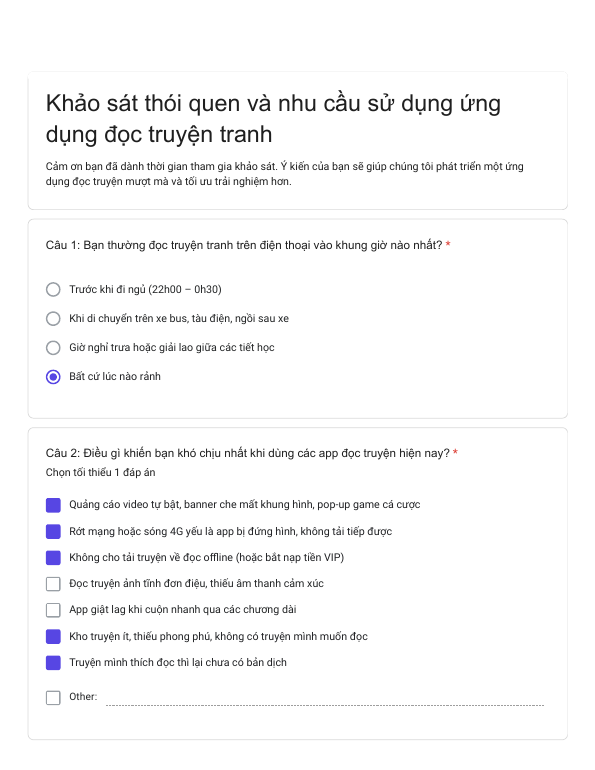
\includegraphics[width=0.95\textwidth,height=7.8cm,keepaspectratio]{figures/survey/p-01.png}}
        \caption{Survey Form -- Questions 1 \& 2 (Respondent 1)}
    \end{subfigure}
    \hfill
    \begin{subfigure}[b]{0.48\textwidth}
        \centering
        \fbox{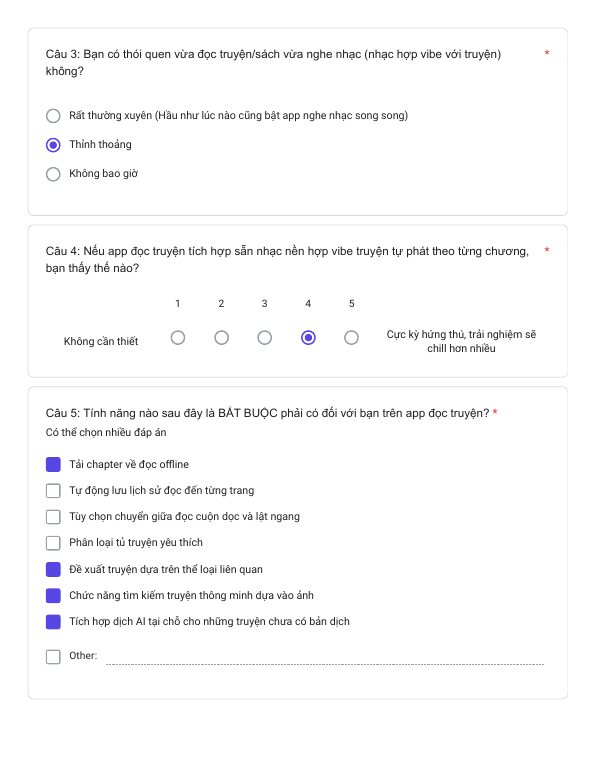
\includegraphics[width=0.95\textwidth,height=7.8cm,keepaspectratio]{figures/survey/p-02.png}}
        \caption{Survey Form -- Questions 3, 4 \& 5 (Respondent 1)}
    \end{subfigure}
    \caption{Sample empirical evidence extracted from the Google Forms user elicitation archive (\texttt{khao\_sat\_4\_nguoi.pdf}).}
    \label{fig:survey_evidence}
\end{figure}

\subsubsection{Quantitative Statistical Synthesis \& Architectural Implications}
Table~\ref{tab:survey_stats} consolidates the quantitative distribution of user pain points and feature demands alongside the concrete engineering decisions derived for \textbf{Naomi}.

\begin{table}[H]
\centering
\caption{Quantitative synthesis of elicitation findings and direct architectural implications.}
\label{tab:survey_stats}
\footnotesize
\renewcommand{\arraystretch}{1.25}
\begin{tabularx}{\textwidth}{L{4.2cm} C{2.0cm} Y}
\toprule
\rowcolor{tablehead}
\textbf{Empirical Finding / Metric} & \textbf{Prevalence} & \textbf{Direct Engineering \& Specification Decision} \\
\midrule
\textbf{Intrusive video/banner/gambling ads} (Q2) & \textbf{100.0\%} ($4/4$) & Strict \textbf{100\% Ad-Free commitment}; zero advertising or tracking SDKs; monetisation/IAP explicitly excluded as \texttt{WON'T-HAVE} (\texttt{FR-15}). \\
\rowcolor{tablerow}
\textbf{Habit of pairing music with reading} (Q3) \& \textbf{Ambient Audio Rating} (Q4) & \textbf{100.0\%} ($4/4$)\newline Mean: \textbf{3.75 / 5.0} & Core differentiator (\textbf{Unique Value Proposition}): integrate \texttt{just\_audio} streaming from Supabase Storage matched to comic genres (\texttt{FR-05}, \texttt{FR-09}, \texttt{UC-04}). \\
\textbf{Missing translations} (Q2) \& \textbf{In-place AI Translation demand} (Q5) & \textbf{75\%--100\%} ($3\text{--}4/4$) & Specify in-place AI chapter translation overlay (\texttt{FR-12}) on the Reader top toolbar (\texttt{S05} Icon $\star$) as a high-value \texttt{COULD-HAVE} capability. \\
\rowcolor{tablerow}
\textbf{Exact page-level reading history} (Q5) & \textbf{75.0\%} ($3/4$) & Persist \texttt{last\_page\_read} and \texttt{read\_percentage} asynchronously in SQLite ($\le 50\text{ ms}$) with bidirectional Supabase cloud sync (\texttt{FR-04}, \texttt{NFR-09}) and surface on the \texttt{S02} Home Hero card. \\
\textbf{Limited catalog} (Q2) \& \textbf{Genre-based recommendations} (Q5) & \textbf{75.0\%} ($3/4$) & Integrate the open \textbf{MangaDex REST API v5} catalog (\texttt{FR-01}, \texttt{FR-08}) with horizontal \textit{Trending} and \textit{Genre} discovery carousels (\texttt{S03}, \texttt{S03b}). \\
\rowcolor{tablerow}
\textbf{Cellular network freezes \& lack of free offline mode} (Q2, Q5) & \textbf{50.0\%} ($2/4$) & Design a \textbf{Hybrid Offline-First Architecture} with full-chapter pre-buffering (\texttt{S10}), 1-tap local chapter downloads (\texttt{FR-06}, \texttt{S11}), and $\le 300\text{ ms}$ offline fallback (\texttt{FR-13}, \texttt{S09} $\to$ \texttt{S07}). \\
\textbf{Scrolling lag on long chapters} (Q2) & \textbf{50.0\%} ($2/4$) & Enforce \textbf{60 FPS rendering} ($\le 16.6\text{ ms/frame}$, \texttt{NFR-03}) via Flutter Impeller/Skia virtualised viewport lists and strict file-system media storage (never storing image BLOBs in SQLite). \\
\rowcolor{tablerow}
\textbf{Visual image search from screenshots} (Q5) & \textbf{50.0\%} ($2/4$) & Provide camera icon trigger on \texttt{S03} invoking the OS \textbf{System Photo Picker} (\texttt{FR-11}), achieving visual search with \textbf{zero storage permissions} (\texttt{NFR-12}). \\
\textbf{Willingness to adopt Naomi over existing apps} (Q6) & \textbf{100.0\%} ($4/4$) & Validates strong product-market fit provided the core Must-Have and Should-Have baseline is delivered cleanly in Assignment 02. \\
\bottomrule
\end{tabularx}
\end{table}

\newpage
\section{Functional Requirements Specification}
\label{sec:functional_requirements}

\subsection{Methodology \& MoSCoW Prioritisation}
\label{subsec:moscow}

To rigorously control project scope, guarantee $100\%$ implementation feasibility in Assignment 02, and maintain direct alignment with the empirical user elicitation findings from Section~\ref{sec:problem_analysis}, all functional requirements of the \textbf{Naomi} platform are classified using the \textbf{MoSCoW Prioritisation Framework}:
\begin{itemize}
    \item \badgeMust{} \textbf{(Core Acceptance Baseline):} Non-negotiable functional capabilities required for the system to operate end-to-end; $100\%$ of Must-Have requirements must pass acceptance verification in Assignment 02.
    \item \badgeShould{} \textbf{(High-Value Experience Enhancers):} Important features that elevate user experience, resilience, and personalisation to a production-grade standard ($90\text{--}100\%$ target rubric band).
    \item \badgeCould{} \textbf{(Innovative Smart Extensions):} Advanced AI/computer-vision capabilities (Visual Search and In-Place AI Chapter Translation) implemented as modular prototypes without compromising core stability.
    \item \badgeWont{} \textbf{(Explicitly Excluded Scope):} Features intentionally omitted from the project boundary to preserve our non-commercial, ad-free, distraction-free \textit{Content-First} philosophy.
\end{itemize}

Table~\ref{tab:fr_matrix} defines the complete catalogue of 17 Functional Requirements (\texttt{FR-00} through \texttt{FR-16}).

\begin{small}
\renewcommand{\arraystretch}{1.28}
\begin{longtable}{C{1.4cm} L{3.6cm} C{2.6cm} p{7.1cm}}
\caption{Master Functional Requirements Matrix with MoSCoW prioritisation (\texttt{FR-00} to \texttt{FR-16}).}
\label{tab:fr_matrix} \\
\toprule
\rowcolor{tablehead}
\textbf{FR ID} & \textbf{Requirement Name} & \textbf{MoSCoW} & \textbf{System Business Capability Description} \\
\midrule
\endfirsthead
\multicolumn{4}{c}{{\bfseries \tablename\ \thetable{} -- continued from previous page}} \\
\toprule
\rowcolor{tablehead}
\textbf{FR ID} & \textbf{Requirement Name} & \textbf{MoSCoW} & \textbf{System Business Capability Description} \\
\midrule
\endhead
\midrule \multicolumn{4}{r}{{Continued on next page}} \\ \bottomrule
\endfoot
\bottomrule
\endlastfoot

\textbf{FR-00} & \textbf{User Account Authentication} & \badgeMust & Enables users to register, sign in, and request password recovery via Email/Password (\texttt{Supabase Auth}). Persists encrypted JWT sessions in hardware-backed storage. Excludes third-party OAuth social logins to maintain provider independence. \\
\rowcolor{tablerow}
\textbf{FR-01} & \textbf{Comic Discovery \& Search (MangaDex API)} & \badgeMust & Searches comics by title or author keyword; organises horizontal discovery rows by \textit{Trending} and \textit{Genre} (\textit{Fantasy, Action}, etc.); supports expanding any row into a full paginated grid (\texttt{S03b}). \\
\textbf{FR-02} & \textbf{Full-Screen Distraction-Free Reader} & \badgeMust & Renders chapter pages across $100\%$ of the viewport; provides a single translucent top icon toolbar for chapter navigation and a 1-tap \textit{Focus Mode} that hides all UI chrome. \\
\rowcolor{tablerow}
\textbf{FR-03} & \textbf{Flexible Dual Reading Mode Toggle} & \badgeMust & Allows instant in-reader switching between continuous vertical scrolling (\textit{Webtoon long-strip mode}) and horizontal paginated flipping (\textit{traditional Manga mode}). \\
\textbf{FR-04} & \textbf{Auto-Save Progress \& Instant Resume} & \badgeMust & Automatically records the exact chapter and page number (\texttt{last\_page\_read}) into local SQLite and synchronises to Supabase Cloud; surfaces a 1-tap \textit{Continue} hero card on the Home screen (\texttt{S02}). \\
\rowcolor{tablerow}
\textbf{FR-05} & \textbf{Genre-Matched Instrumental Ambient Audio} & \badgeMust & Automatically recommends and streams instrumental background audio tracks matching the primary genre of the active comic to foster an immersive, relaxing reading atmosphere. \\
\textbf{FR-06} & \textbf{Offline Chapter Download} & \badgeMust & Downloads all page image assets of selected chapters to sandboxed device storage for offline reading; displays real-time percentage and byte progress (\texttt{S11}). \\
\rowcolor{tablerow}
\textbf{FR-07} & \textbf{Personal Library Management} & \badgeMust & Provides a dedicated two-button Library hub (\texttt{S07}) separating \textit{Favorites} (cloud-synced bookmarked series) and \textit{Offline Reading} (locally saved chapters with storage footprint metrics). \\
\textbf{FR-08} & \textbf{Consolidated Home Feed \& Recommendations} & \badgeShould & Presents a streamlined three-block Home screen (\texttt{S02}): (1) \textit{Continue Reading} hero card, (2) \textit{Recent} horizontal carousel, and (3) \textit{Recommended} horizontal carousel based on genres. \\
\rowcolor{tablerow}
\textbf{FR-09} & \textbf{Minimalist Audio Sheet Controls} & \badgeShould & Provides a clean bottom sheet (\texttt{S06}) with Play/Pause toggle, continuous volume slider, and track selection among genre-matched instrumentals; auto-pauses on phone calls or app backgrounding. \\
\textbf{FR-10} & \textbf{Comic Detail View \& Quick Chapter Actions} & \badgeShould & Displays complete comic metadata (cover, author, rating, genres, synopsis), four primary action buttons (\textit{Read First, Read Latest, Favorite, Download}), and the full chapter list (\texttt{S04}). \\
\rowcolor{tablerow}
\textbf{FR-11} & \textbf{Smart Visual Search via System Photo Picker} & \badgeCould & Allows users to select a comic panel screenshot via the OS \texttt{System Photo Picker} (requiring zero storage permissions) to identify the matching series (\texttt{S03}). \\
\textbf{FR-12} & \textbf{In-Place AI Chapter Translation} & \badgeCould & Integrates an on-demand AI translation action (\texttt{S05} Icon $\star$) that translates dialogue text across the currently open chapter into the user's target language. \\
\rowcolor{tablerow}
\textbf{FR-13} & \textbf{Offline Network Loss Fallback} & \badgeShould & Detects loss of Internet connectivity when opening an uncached chapter, displays a friendly offline error state (\texttt{S09}), and provides a direct CTA button routing to the Offline Library (\texttt{S07}). \\
\textbf{FR-14} & \textbf{User Profile \& System Settings Customisation} & \badgeShould & Manages user profile details, appearance theme (\textit{System / Light / Dark}), UI language (\textit{English / Vietnamese}), disk cache inspection/clearing, notification toggles, and sign-out (\texttt{S08}). \\
\rowcolor{tablerow}
\textbf{FR-15} & \textbf{In-App Purchases (IAP) \& Virtual Coins} & \badgeWont & Explicitly excluded to uphold a $100\%$ non-commercial, paywall-free reading environment. \\
\textbf{FR-16} & \textbf{In-App Social Feed \& 1-on-1 Direct Messaging} & \badgeWont & Explicitly excluded to eliminate social clutter and keep architectural complexity focused on reading performance. \\
\end{longtable}
\end{small}

\subsection{System Use Case Diagram}
\label{subsec:use_case_diagram}

Figure~\ref{fig:use_case_diagram} illustrates the UML 2.5 Use Case Diagram modelling all interactions between the primary human actor (\textbf{Reader}), the nine core use cases (\texttt{UC-00} to \texttt{UC-08}) inside the \textbf{Naomi Mobile Application} boundary, and the two external system actors (\textbf{Supabase Backend} and \textbf{MangaDex REST API}). Mandatory sub-flows are linked via \texttt{<<include>>} dependencies (\texttt{UC-03} includes \texttt{UC-05}), while optional contextual enrichments are modelled via \texttt{<<extend>>} dependencies (\texttt{UC-04} extends \texttt{UC-03}; \texttt{UC-02} extends \texttt{UC-01}; \texttt{UC-06} extends \texttt{UC-07}).

\begin{figure}[H]
    \centering
    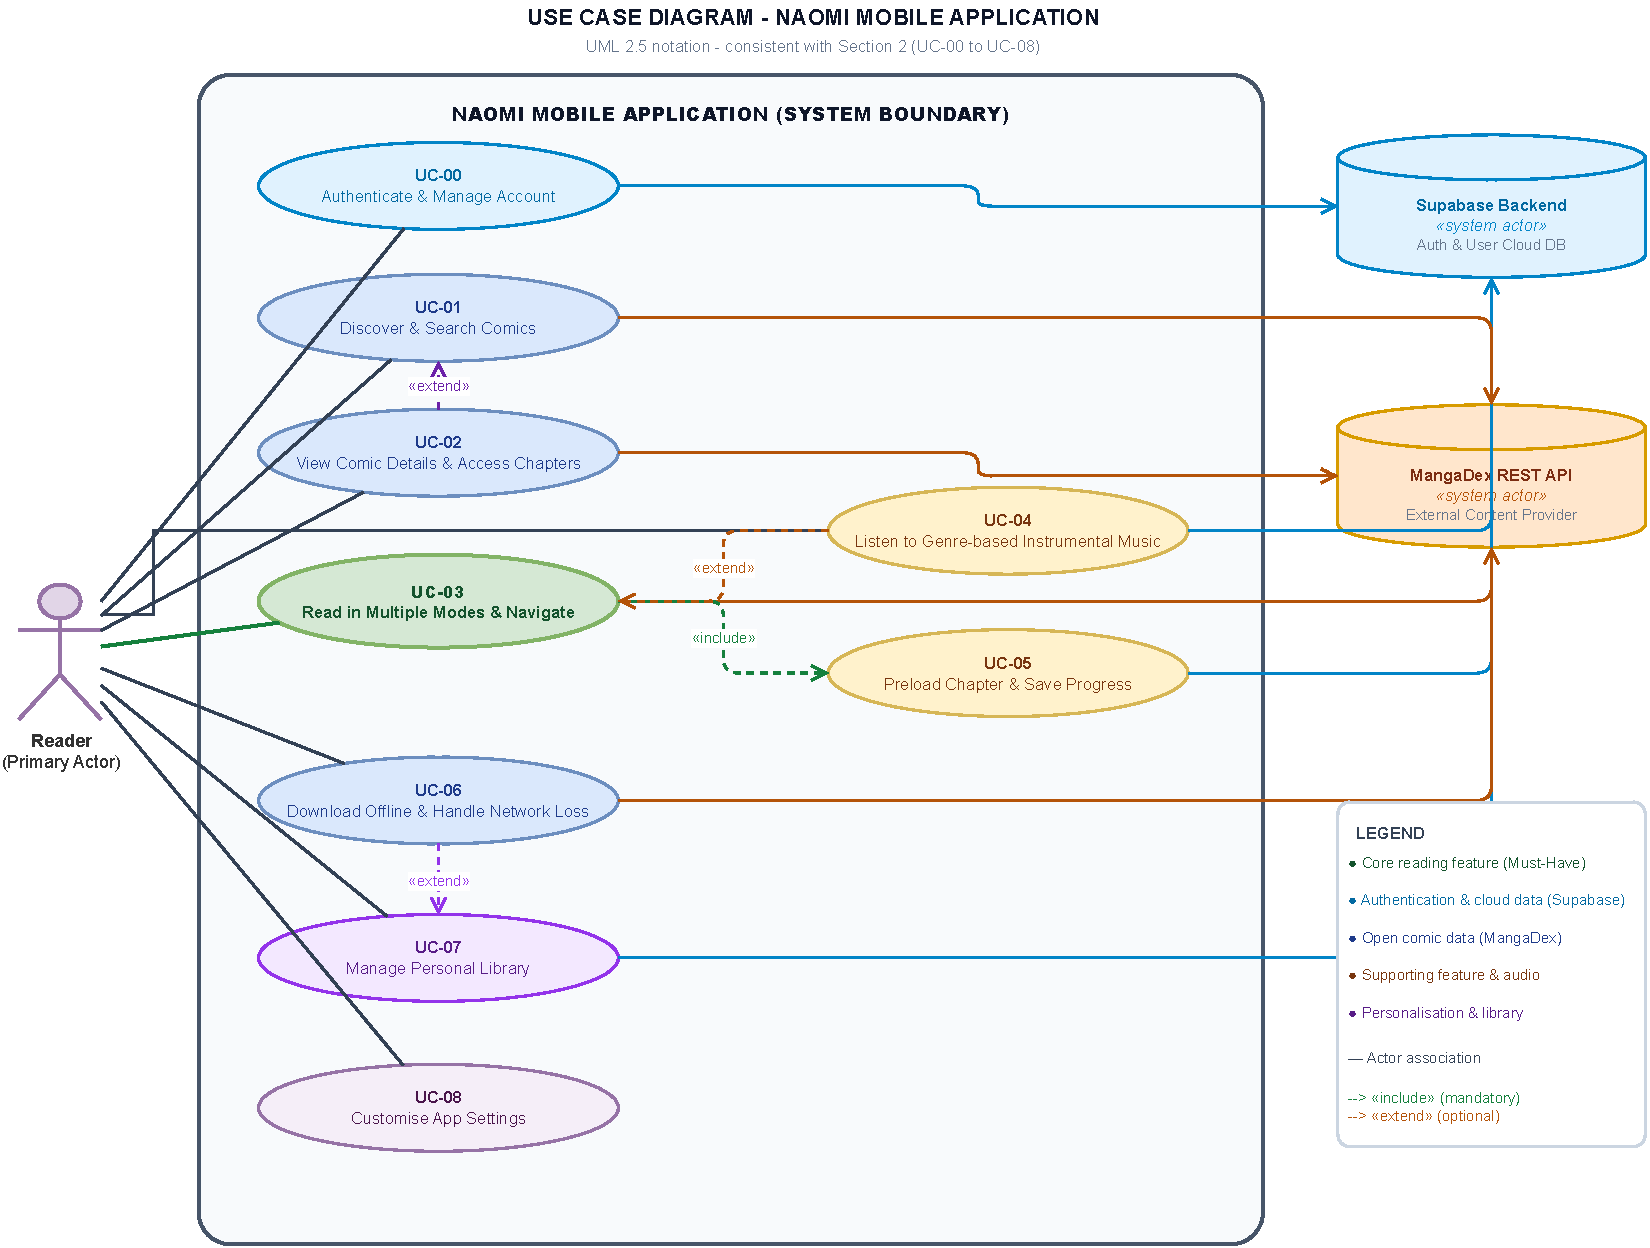
\includegraphics[width=0.98\textwidth]{figures/diagrams/use_case_diagram.pdf}
    \caption{UML 2.5 System Use Case Diagram for the Naomi Mobile Application (\texttt{UC-00} to \texttt{UC-08}).}
    \label{fig:use_case_diagram}
\end{figure}

\subsection{Detailed Use Case Specifications}
\label{subsec:use_case_specs}

Table~\ref{tab:uc_summary} summarises the scope of the nine system use cases, followed by their complete structured specifications (Actors, Preconditions, Postconditions, Main Success Scenario, Alternative Flows, and Exception Flows).

\begin{table}[H]
\centering
\caption{Overview of the nine system Use Cases (\texttt{UC-00} to \texttt{UC-08}).}
\label{tab:uc_summary}
\footnotesize
\renewcommand{\arraystretch}{1.22}
\begin{tabularx}{\textwidth}{C{1.4cm} L{4.6cm} C{2.3cm} Y}
\toprule
\rowcolor{tablehead}
\textbf{UC ID} & \textbf{Use Case Name} & \textbf{Primary Actor} & \textbf{Business Goal} \\
\midrule
\textbf{UC-00} & Authenticate \& Manage Account & Reader & Sign up, sign in, or reset password via Email/Password; persist encrypted JWT session via Supabase Auth. \\
\rowcolor{tablerow}
\textbf{UC-01} & Discover \& Search Comics & Reader & Search comics by keyword, browse \textit{Trending} and \textit{Genre} rows, expand full lists, or search by image (\texttt{FR-11}). \\
\textbf{UC-02} & View Comic Details \& Access Chapters & Reader & Inspect comic metadata, trigger \textit{Read First / Read Latest}, bookmark to \textit{Favorites}, or initiate chapter downloads. \\
\rowcolor{tablerow}
\textbf{UC-03} & Read in Multiple Modes \& Navigate & Reader & Read full-screen pages, toggle Vertical Webtoon $\leftrightarrow$ Horizontal Manga, switch chapters, and activate \textit{Focus Mode}. \\
\textbf{UC-04} & Listen to Genre-Based Instrumental Music & Reader & Stream instrumental ambient tracks matched to the comic's genre; control playback, volume, and track selection. \\
\rowcolor{tablerow}
\textbf{UC-05} & Preload Chapter \& Save Progress & System / Reader & Pre-buffer $100\%$ of chapter pages before opening the reader (\texttt{S10}); continuously persist page progress to SQLite \& Cloud. \\
\textbf{UC-06} & Download Offline \& Handle Network Loss & Reader & Download chapter page assets into sandboxed local storage (\texttt{S11}); route gracefully to Offline Library on network loss (\texttt{S09}). \\
\rowcolor{tablerow}
\textbf{UC-07} & Manage Personal Library & Reader & Access and manage the two-button Personal Library (\texttt{S07}): cloud-synced \textit{Favorites} and local \textit{Offline Reading}. \\
\textbf{UC-08} & Customise App Settings & Reader & Configure appearance theme (\textit{System/Light/Dark}), UI language, disk cache cleanup, notifications, and sign-out (\texttt{S08}). \\
\bottomrule
\end{tabularx}
\end{table}

\subsubsection{UC-00: Authenticate \& Manage User Account}
\begin{table}[H]
\footnotesize
\renewcommand{\arraystretch}{1.22}
\begin{tabularx}{\textwidth}{L{3.2cm} Y}
\toprule
\rowcolor{tablehead}
\textbf{Field} & \textbf{Specification Details} \\
\midrule
\textbf{Use Case ID \& Name} & \textbf{UC-00: Authenticate \& Manage User Account} (Maps to \texttt{FR-00}, \texttt{NFR-05}, \texttt{NFR-10}) \\
\textbf{Primary / Secondary Actors} & \textbf{Primary:} Reader \quad|\quad \textbf{Secondary:} Supabase Auth Server (\texttt{POST /auth/v1/token}) \\
\textbf{Preconditions} & Device has active Internet connectivity; user is unauthenticated on screen \texttt{S01} (\textit{Sign In}). \\
\textbf{Postconditions} & Authenticated session is established; JWT \texttt{access\_token} and \texttt{refresh\_token} are encrypted via AES-256 in \texttt{FlutterSecureStorage} (Android Keystore / iOS Keychain). \\
\textbf{Main Success Flow (Sign In)} &
\begin{enumerate}[nosep,leftmargin=1.4em]
    \item User opens the application and lands on the \textit{Sign In} screen (\texttt{S01}).
    \item User enters a valid email address and password and taps \textbf{Sign In}.
    \item System validates input syntax client-side (RFC 5322 email format, non-empty password).
    \item System dispatches an HTTPS TLS 1.3 authentication request to Supabase Auth (\texttt{API 04}).
    \item Upon receiving \texttt{HTTP 200 OK} ($\le 1.0\text{ s}$), system stores the JWT pair in \texttt{FlutterSecureStorage}, loads the user profile, and navigates to the \textit{Home} screen (\texttt{S02}).
\end{enumerate} \\
\textbf{Alternative Flows} &
\begin{itemize}[nosep,leftmargin=1.4em]
    \item \textbf{00a -- Account Registration (\textit{Sign Up}):} User taps \textit{Sign Up} on \texttt{S01} $\to$ submits valid email and new password $\to$ system calls \texttt{POST /auth/v1/signup}, creates the \texttt{users} profile row via database trigger/upsert, and signs the user in automatically.
    \item \textbf{00b -- Password Recovery (\textit{Forgot Password?}):} User taps \textit{Forgot Password?} $\to$ enters registered email $\to$ Supabase dispatches a password reset link via email.
    \item \textbf{00c -- Auto-Login on Warm/Cold Launch:} If a valid token exists in \texttt{FlutterSecureStorage}, \texttt{AuthBloc} restores the session silently and opens \texttt{S02} directly ($\le 0.8\text{ s}$ warm start).
\end{itemize} \\
\textbf{Exception Flows} &
\begin{itemize}[nosep,leftmargin=1.4em]
    \item \textbf{00e -- Invalid Credentials (\texttt{HTTP 400}):} System displays an inline validation message (\textit{``Invalid email or password''}) while preserving the typed email address for correction.
\end{itemize} \\
\bottomrule
\end{tabularx}
\end{table}

\subsubsection{UC-01: Discover \& Search Comics}
\begin{table}[H]
\footnotesize
\renewcommand{\arraystretch}{1.22}
\begin{tabularx}{\textwidth}{L{3.2cm} Y}
\toprule
\rowcolor{tablehead}
\textbf{Field} & \textbf{Specification Details} \\
\midrule
\textbf{Use Case ID \& Name} & \textbf{UC-01: Discover \& Search Comics} (Maps to \texttt{FR-01}, \texttt{FR-11}, \texttt{NFR-12}) \\
\textbf{Primary / Secondary Actors} & \textbf{Primary:} Reader \quad|\quad \textbf{Secondary:} MangaDex REST API v5 (\texttt{GET /manga}) \\
\textbf{Preconditions} & User navigates to the \textit{Discover} tab (\texttt{S03}). \\
\textbf{Postconditions} & Matching comics or expanded category grids (\texttt{S03b}) are rendered with real cover artwork. \\
\textbf{Main Success Flow} &
\begin{enumerate}[nosep,leftmargin=1.4em]
    \item User selects the \textit{Discover} tab (\texttt{S03}) from the bottom navigation bar.
    \item System queries \texttt{GET /manga} (\texttt{API 01}) to populate horizontal scroll carousels for \textbf{Trending} and specific \textbf{Genres} (\textit{Fantasy, Action}, etc.).
    \item User either types a query into the search bar (\textit{``Search titles, authors...''}) or taps the expand chevron (\texttt{>}) next to any section header.
    \item System transitions to the \textit{Expanded List} screen (\texttt{S03b}), displaying a 2-column vertical grid of matching titles with infinite pagination.
\end{enumerate} \\
\textbf{Alternative Flows} &
\begin{itemize}[nosep,leftmargin=1.4em]
    \item \textbf{01a -- Zero-Permission Visual Search (\texttt{FR-11}):} User taps the Camera icon inside the \texttt{S03} search bar $\to$ system invokes the OS \texttt{System Photo Picker} (requiring zero storage permissions) $\to$ user selects a comic panel screenshot $\to$ system extracts visual features/title match and displays the corresponding comic result.
\end{itemize} \\
\textbf{Exception Flows} &
\begin{itemize}[nosep,leftmargin=1.4em]
    \item \textbf{01e -- Empty Result or Rate Limit (\texttt{HTTP 429}):} If no titles match, system renders a clean Empty State; if MangaDex returns \texttt{HTTP 429}, the \texttt{Dio} interceptor applies exponential backoff automatically.
\end{itemize} \\
\bottomrule
\end{tabularx}
\end{table}

\subsubsection{UC-02: View Comic Details \& Access Chapters}
\begin{table}[H]
\footnotesize
\renewcommand{\arraystretch}{1.22}
\begin{tabularx}{\textwidth}{L{3.2cm} Y}
\toprule
\rowcolor{tablehead}
\textbf{Field} & \textbf{Specification Details} \\
\midrule
\textbf{Use Case ID \& Name} & \textbf{UC-02: View Comic Details \& Access Chapters} (Maps to \texttt{FR-10}, \texttt{FR-06}, \texttt{FR-07}) \\
\textbf{Primary / Secondary Actors} & \textbf{Primary:} Reader \quad|\quad \textbf{Secondary:} MangaDex API (\texttt{GET /manga/\{id\}/feed}) \& Supabase \\
\textbf{Preconditions} & User taps a comic card on \textit{Home} (\texttt{S02}), \textit{Discover} (\texttt{S03}/\texttt{S03b}), or \textit{Library} (\texttt{S07}). \\
\textbf{Postconditions} & Comic metadata and chapter list are displayed on \texttt{S04}; bookmark or download actions are persisted. \\
\textbf{Main Success Flow} &
\begin{enumerate}[nosep,leftmargin=1.4em]
    \item User taps a comic card (e.g., \textit{Frieren: Beyond Journey's End}).
    \item System opens \textit{Manga Detail} (\texttt{S04}) and fetches metadata plus the chapter feed (\texttt{API 02}).
    \item System renders cover art, title, author/artist, star rating ($\star\ 4.9$), genre tags, synopsis, the 4-button action bar (\textbf{Read First}, \textbf{Read Latest}, \textbf{$\heartsuit$ Favorite}, \textbf{$\downarrow$ Download}), and the chapter list showing saved/read badges.
    \item User taps \textbf{Read First}, \textbf{Read Latest}, or any specific chapter row to begin reading (invoking \texttt{UC-05} $\to$ \texttt{UC-03}).
\end{enumerate} \\
\textbf{Alternative Flows} &
\begin{itemize}[nosep,leftmargin=1.4em]
    \item \textbf{02a -- Toggle Favorite Bookmark:} User taps \textbf{$\heartsuit$ Favorite} $\to$ button highlights in soft coral red (\texttt{\#E05353}), upserting into local SQLite \texttt{bookmarks} and syncing to Supabase (\texttt{API 06}).
\end{itemize} \\
\bottomrule
\end{tabularx}
\end{table}

\subsubsection{UC-03: Read in Multiple Modes \& Navigate}
\begin{table}[H]
\footnotesize
\renewcommand{\arraystretch}{1.22}
\begin{tabularx}{\textwidth}{L{3.2cm} Y}
\toprule
\rowcolor{tablehead}
\textbf{Field} & \textbf{Specification Details} \\
\midrule
\textbf{Use Case ID \& Name} & \textbf{UC-03: Read in Multiple Modes \& Navigate} (Maps to \texttt{FR-02}, \texttt{FR-03}, \texttt{FR-12}, \texttt{NFR-03}) \\
\textbf{Primary / Secondary Actors} & \textbf{Primary:} Reader \quad|\quad \textbf{Included UC:} \texttt{UC-05} (Preload \& Save Progress) \\
\textbf{Preconditions} & Chapter pages have been pre-buffered via \texttt{S10} (\texttt{UC-05}) or loaded from local offline storage. \\
\textbf{Postconditions} & User reads at $\ge 60\text{ FPS}$; reading mode preference and current page index are saved continuously. \\
\textbf{Main Success Flow} &
\begin{enumerate}[nosep,leftmargin=1.4em]
    \item System opens the \textit{Full Screen Reader} (\texttt{S05}) with artwork occupying $100\%$ of the viewport over an AMOLED dark background (\texttt{\#111116}).
    \item A single translucent top toolbar (\texttt{rgba(22,22,28,0.90)}) provides icon-only controls:
    \begin{itemize}[nosep]
        \item \textbf{Back (\texttt{<}):} Returns to \texttt{S04} or \texttt{S02}.
        \item \textbf{Chapter Switcher (\texttt{< Ch.\ 24 $\blacktriangledown$ >}):} Steps to previous/next chapter or opens a dropdown to jump directly to any chapter.
        \item \textbf{Music Icon (\musicnote):} Opens the \textit{Audio Sheet} (\texttt{S06}, invoking \texttt{UC-04}).
        \item \textbf{Focus Mode Icon ($\odot$):} Hides the top toolbar completely for $100\%$ unobstructed artwork viewing; tapping the canvas restores the toolbar.
        \item \textbf{Language Icon ($\oplus$):} Selects target translation/UI language.
        \item \textbf{AI Translate Icon ($\star$ -- \texttt{FR-12}):} Translates dialogue in the current chapter into the selected language in-place.
        \item \textbf{Reader Mode Toggle Icon ($\leftrightarrows$ -- \texttt{FR-03}):} Switches instantly between continuous Vertical Webtoon Scroll and Horizontal Manga Page Flip.
    \end{itemize}
\end{enumerate} \\
\textbf{Exception Flows} &
\begin{itemize}[nosep,leftmargin=1.4em]
    \item \textbf{03e -- Mid-Chapter Network Drop:} Because $100\%$ of the active chapter was pre-buffered in \texttt{UC-05}, the user continues reading the entire chapter without interruption.
\end{itemize} \\
\bottomrule
\end{tabularx}
\end{table}

\subsubsection{UC-04: Listen to Genre-Based Instrumental Music}
\begin{table}[H]
\footnotesize
\renewcommand{\arraystretch}{1.22}
\begin{tabularx}{\textwidth}{L{3.2cm} Y}
\toprule
\rowcolor{tablehead}
\textbf{Field} & \textbf{Specification Details} \\
\midrule
\textbf{Use Case ID \& Name} & \textbf{UC-04: Listen to Genre-Based Instrumental Music} (Maps to \texttt{FR-05}, \texttt{FR-09}, \texttt{NFR-16}, \texttt{NFR-17}) \\
\textbf{Primary / Secondary Actors} & \textbf{Primary:} Reader \quad|\quad \textbf{Secondary:} Supabase Storage \& DB (\texttt{GET /rest/v1/ambient\_tracks}) \\
\textbf{Preconditions} & User is actively reading a chapter in \texttt{S05} and taps the Music icon (\musicnote). \\
\textbf{Postconditions} & Selected instrumental track loops smoothly at the chosen volume or pauses cleanly. \\
\textbf{Main Success Flow} &
\begin{enumerate}[nosep,leftmargin=1.4em]
    \item User taps the Music icon (\musicnote) on the \texttt{S05} top toolbar.
    \item System slides up the minimalist \textit{Audio Sheet} (\texttt{S06}) over the dimmed reader canvas.
    \item System displays the active instrumental track matched to the comic's genre (e.g., \textit{``Winds of Aureole (Instrumental)''} for \textit{Fantasy}), a $44\text{ px}$ circular Play/Pause button, a continuous volume slider (defaulting to a gentle $30\%$), and a 3-track list of related genre instrumentals.
    \item User adjusts volume, pauses/resumes, or taps another track in the list to switch audio immediately while continuing to read.
\end{enumerate} \\
\textbf{Exception Flows} &
\begin{itemize}[nosep,leftmargin=1.4em]
    \item \textbf{04e -- Audio Focus Loss (Phone Call / App Backgrounded):} \texttt{AudioSession} detects OS focus loss and pauses playback within $\le 100\text{ ms}$ (\texttt{NFR-17}) to prevent audio conflict and battery drain.
\end{itemize} \\
\bottomrule
\end{tabularx}
\end{table}

\subsubsection{UC-05: Preload Chapter Data \& Save Reading Progress}
\begin{table}[H]
\footnotesize
\renewcommand{\arraystretch}{1.22}
\begin{tabularx}{\textwidth}{L{3.2cm} Y}
\toprule
\rowcolor{tablehead}
\textbf{Field} & \textbf{Specification Details} \\
\midrule
\textbf{Use Case ID \& Name} & \textbf{UC-05: Preload Chapter Data \& Save Reading Progress} (Maps to \texttt{FR-02}, \texttt{FR-04}, \texttt{NFR-04}, \texttt{NFR-09}) \\
\textbf{Primary / Secondary Actors} & \textbf{Primary:} System / Reader \quad|\quad \textbf{Secondary:} MangaDex@Home CDN (\texttt{API 03}) \& Supabase (\texttt{API 05}) \\
\textbf{Preconditions} & User triggers chapter opening from \texttt{S02} (\textit{Continue}) or \texttt{S04} (\textit{Manga Detail}). \\
\textbf{Postconditions} & All chapter pages are pre-buffered in cache; \texttt{reading\_history} is updated locally and queued for cloud sync. \\
\textbf{Main Success Flow} &
\begin{enumerate}[nosep,leftmargin=1.4em]
    \item System displays the \textit{Full Chapter Preload} screen (\texttt{S10}) over an AMOLED dark backdrop with a pulsing cover thumbnail and progress bar (\textit{``Loading full chapter... 42 / 42 pages ready (100\%)''}).
    \item If the chapter is already saved offline in SQLite, \texttt{S10} completes instantaneously; otherwise, system resolves \texttt{GET /at-home/server/\{chapterId\}} ($\le 1.5\text{ s}$ initial latency) and pre-buffers all chapter pages concurrently.
    \item Upon reaching $100\%$, system transitions automatically to \texttt{S05} at the user's last read page (e.g., Page 18/42).
    \item As the user scrolls or flips pages, \texttt{ReaderBloc} writes \texttt{last\_page\_read} and \texttt{read\_percentage} asynchronously to local SQLite ($\le 50\text{ ms}$) and upserts to Supabase (\texttt{API 05}).
\end{enumerate} \\
\bottomrule
\end{tabularx}
\end{table}

\subsubsection{UC-06: Download Chapter Offline \& Handle Network Loss}
\begin{table}[H]
\footnotesize
\renewcommand{\arraystretch}{1.22}
\begin{tabularx}{\textwidth}{L{3.2cm} Y}
\toprule
\rowcolor{tablehead}
\textbf{Field} & \textbf{Specification Details} \\
\midrule
\textbf{Use Case ID \& Name} & \textbf{UC-06: Download Chapter Offline \& Handle Network Loss} (Maps to \texttt{FR-06}, \texttt{FR-13}, \texttt{NFR-08}) \\
\textbf{Primary / Secondary Actors} & \textbf{Primary:} Reader \quad|\quad \textbf{Secondary:} MangaDex@Home CDN \& Local Sandboxed Storage \\
\textbf{Preconditions} & User views a comic on \texttt{S04} or attempts to open an uncached chapter while offline. \\
\textbf{Postconditions} & Chapter images are persisted in \texttt{ApplicationDocumentsDirectory} and registered in \texttt{offline\_downloads}; or user is routed cleanly to \texttt{S07} during network loss. \\
\textbf{Main Success Flow (Download)} &
\begin{enumerate}[nosep,leftmargin=1.4em]
    \item On \texttt{S04}, user taps \textbf{$\downarrow$ Download} or the download arrow on a specific chapter row (e.g., Ch.\ 24).
    \item System transitions to \texttt{S11} (\textit{Download in Progress}), streaming image bytes sequentially to sandboxed storage while displaying a green progress bar (\textit{``Downloading... 24.5 MB / 36 MB -- 68\%''}) and bottom toast notification.
    \item Upon completion, system updates SQLite \texttt{offline\_downloads.download\_status = 'completed'} and marks the chapter badge as \textbf{Saved}.
\end{enumerate} \\
\textbf{Exception Flow (Offline Fallback)} &
\begin{itemize}[nosep,leftmargin=1.4em]
    \item \textbf{06e -- Network Disconnected on Uncached Chapter (\texttt{S09}):} If the device has no Internet connection and the requested chapter is not in \texttt{offline\_downloads}, system detects offline status within $\le 300\text{ ms}$ (\texttt{NFR-08}), displays \texttt{S09} (\textit{``Oops! No internet connection''}), and provides the primary CTA button \textbf{Go to Offline Library}, routing directly to \texttt{S07}.
\end{itemize} \\
\bottomrule
\end{tabularx}
\end{table}

\subsubsection{UC-07: Manage Personal Library \& UC-08: Customise App Settings}
\begin{table}[H]
\footnotesize
\renewcommand{\arraystretch}{1.22}
\begin{tabularx}{\textwidth}{L{3.2cm} Y}
\toprule
\rowcolor{tablehead}
\textbf{Field} & \textbf{Specification Details} \\
\midrule
\textbf{UC-07: Manage Personal Library} &
\begin{itemize}[nosep,leftmargin=1.4em]
    \item \textbf{Goal \& Mapping:} Centralised personal collection hub (\texttt{FR-07}, Screen \texttt{S07}).
    \item \textbf{Main Flow:} User taps the \textit{Library} tab (\texttt{S07}). System renders exactly two large $20\text{ px}$-radius action cards:
    \begin{enumerate}[nosep]
        \item \textbf{Favorites ($\heartsuit$ -- \textit{``12 stories marked''}):} Opens the cloud-synced list of bookmarked series from Supabase/SQLite.
        \item \textbf{Offline Reading ($\downarrow$ -- \textit{``8 chapters saved $\cdot$ 280 MB''}):} Opens locally downloaded chapters available for zero-network reading and allows single-chapter deletion to free disk space.
    \end{enumerate}
\end{itemize} \\
\midrule
\textbf{UC-08: Customise App Settings} &
\begin{itemize}[nosep,leftmargin=1.4em]
    \item \textbf{Goal \& Mapping:} Personalise system preferences and manage storage/session (\texttt{FR-14}, \texttt{NFR-07}, Screen \texttt{S08}).
    \item \textbf{Main Flow:} User taps the \textit{Profile} tab (\texttt{S08}), displaying user identity (\textit{Kiet Nguyen -- reader.kiet@gmail.com}) and five configuration controls: (1) \textbf{Appearance} segmented control (\textit{System / Light / Dark}), (2) \textbf{Language} selector (\textit{English / Tieng Viet}), (3) \textbf{Storage \& Cache} indicator (\textit{142 MB cached}) with 1-tap \textit{Clear Cache} button, (4) \textbf{Notifications} toggle switch, and (5) \textbf{Sign Out} action (wiping JWT tokens from \texttt{FlutterSecureStorage} and returning to \texttt{S01}).
\end{itemize} \\
\bottomrule
\end{tabularx}
\end{table}

\subsection{User Stories \& Testable Acceptance Criteria (Gherkin BDD)}
\label{subsec:user_stories}

To establish an unambiguous, directly verifiable baseline for Assignment 02 Unit and Acceptance Testing (Rubric Criterion 1.2 \& 2.5), every Use Case is formalised into a User Story accompanied by \textbf{Behaviour-Driven Development (BDD)} scenarios in standard \texttt{Given-When-Then} Gherkin syntax.

\begin{lstlisting}[language=gherkin,caption={US-00 \& US-01: Authentication and Comic Discovery Acceptance Criteria.}]
Feature: US-00 User Account Authentication (Maps to FR-00, UC-00, S01)
  As a mobile reader, I want to sign in, sign up, or recover my password via Email
  So that my bookmarks and page-level reading history sync securely across devices.

  Scenario: Successful sign-in with valid credentials
    Given the user is on the "S01 Sign In" screen
    When the user enters email "reader.kiet@gmail.com" and a valid password
    And taps the "Sign In" button
    Then the system authenticates via Supabase Auth within 1.0 second
    And encrypts the JWT access and refresh tokens inside FlutterSecureStorage
    And navigates the user to the "S02 Home" screen

  Scenario: New account registration and automatic session start
    Given the user is on the "S01 Sign In" screen and taps "Sign Up"
    When the user submits a valid new email and password
    Then the system creates a new account on Supabase Auth and inserts a "users" record
    And automatically establishes an authenticated session on "S02 Home"

Feature: US-01 Comic Discovery, Expanded Lists & Visual Search (Maps to FR-01, FR-11, UC-01, S03, S03b)
  As an exploratory reader, I want to search comics by text or screenshot and browse Trending/Genres
  So that I can quickly find compelling series to read.

  Scenario: Browsing Trending and Genre carousels and expanding full lists
    Given the user is on the "S03 Discover" screen
    When the user views the discovery sections
    Then horizontal carousels for "Trending" and genres ("Fantasy", "Action") are displayed
    When the user taps the expand chevron ">" next to "Trending"
    Then the system opens "S03b Expanded List" displaying a full 2-column paginated grid

  Scenario: Zero-permission Visual Search via System Photo Picker
    Given the user taps the Camera icon inside the "S03 Discover" search bar
    When the OS System Photo Picker opens without requesting storage permissions
    And the user selects a saved manga panel screenshot
    Then the system queries matching visual metadata and displays the corresponding comic series
\end{lstlisting}

\begin{lstlisting}[language=gherkin,caption={US-02, US-03, US-04 \& US-05: Detail View, Full-Screen Reader, Ambient Audio, and Preload.}]
Feature: US-02 Comic Detail View & Quick Chapter Actions (Maps to FR-10, UC-02, S04)
  As a reader, I want to inspect comic metadata and trigger Read First, Read Latest, Favorite, or Download
  So that I can jump into reading or bookmark the series immediately.

  Scenario: Launching Read First or Read Latest and bookmarking to Favorites
    Given the user opens "Frieren: Beyond Journey's End" on "S04 Manga Detail"
    When the user taps "Read First" (or "Read Latest")
    Then the system initiates preloading ("S10") for Chapter 1 (or the latest chapter)
    When the user taps the "Favorite" button
    Then the comic is saved to local SQLite "bookmarks" and synced to Supabase Cloud

Feature: US-03 Full-Screen Dual-Mode Reader & Focus Mode (Maps to FR-02, FR-03, FR-12, UC-03, S05)
  As an immersed reader, I want a 100% full-screen canvas with Focus Mode and Vertical/Horizontal toggle
  So that I can read comfortably at 60 FPS without visual clutter.

  Scenario: Toggling Focus Mode and switching between Vertical Webtoon and Horizontal Manga modes
    Given the user is reading Chapter 24 on "S05 Full Screen Reader"
    When the user taps the Focus Mode icon on the top toolbar
    Then the top toolbar hides completely leaving 100% unobstructed manga artwork
    When the user taps the canvas to restore the toolbar and taps the Reader Mode Toggle icon
    Then the reader switches smoothly between Vertical Scroll and Horizontal Page Flip

Feature: US-04 Genre-Matched Instrumental Ambient Audio (Maps to FR-05, FR-09, UC-04, S06)
  As a late-night reader, I want instrumental music automatically matched to the comic's genre
  So that I can enjoy an atmospheric reading session without running external music apps.

  Scenario: Controlling genre-matched instrumental playback in the Audio Sheet
    Given the user is reading a "Fantasy" comic on "S05" and taps the Music icon
    When the "S06 Audio Sheet" slides up
    Then the system streams the recommended Fantasy instrumental track ("Winds of Aureole")
    And allows pausing/resuming, sliding volume, or tapping another track in the genre list

Feature: US-05 Full-Chapter Pre-buffering & Page-Level Progress Sync (Maps to FR-04, UC-05, S10, S02)
  As a reader, I want all pages of a chapter preloaded before reading and my exact page saved automatically
  So that scrolling never stutters and I can resume instantly from the Home screen.

  Scenario: Pre-buffering 100% of chapter pages and auto-saving page progress
    Given the user selects a 42-page chapter to read
    When "S10 Full Chapter Preload" runs
    Then the progress bar advances to "42 / 42 pages ready (100%)" before opening "S05"
    When the user scrolls to Page 18 and exits the app
    Then "last_page_read = 18" (43%) is saved to SQLite within 50ms and synced to the "S02" Continue card
\end{lstlisting}

\begin{lstlisting}[language=gherkin,caption={US-06, US-07 \& US-08: Offline Downloads, Network Fallback, Library, and Settings.}]
Feature: US-06 Offline Chapter Download & Network Loss Fallback (Maps to FR-06, FR-13, UC-06, S09, S11)
  As a commuting reader, I want to download chapters for offline reading and be guided to my offline library when connectivity drops
  So that weak 4G never interrupts my entertainment.

  Scenario: Downloading a chapter with real-time progress and handling offline errors gracefully
    Given the user taps "Download" on Chapter 24 in "S04"
    Then "S11 Download in Progress" displays real-time progress ("68% - 24.5 MB / 36 MB") until marked "Saved"
    Given the device subsequently loses all Internet connectivity
    When the user taps an uncached chapter
    Then the system transitions within 300ms to "S09 Offline Error State" ("Oops! No internet connection")
    And tapping "Go to Offline Library" routes the user directly to "S07 Library"

Feature: US-07 & US-08 Personal Library & System Settings (Maps to FR-07, FR-14, UC-07, UC-08, S07, S08)
  As a user, I want a clean two-button Library and configurable Theme, Language, and Cache settings
  So that I can manage my collection and device storage effortlessly.

  Scenario: Navigating the two-button Library and switching Appearance Theme
    Given the user opens "S07 Library"
    Then two primary cards ("Favorites" and "Offline Reading") are displayed with item counts and MB size
    Given the user navigates to "S08 Profile & Settings" and selects "Dark" under Appearance
    Then the application theme updates immediately and persists in user preferences
\end{lstlisting}

\newpage
\section{Non-Functional Requirements \& Mobile Constraints}
\label{sec:nfr}

\subsection{SMART Non-Functional Design Philosophy}
\label{subsec:nfr_philosophy}

Delivering functional features alone is insufficient for a media-intensive mobile entertainment application such as \textbf{Naomi}. Mobile devices operate under strict physical and operating-system constraints: \textbf{finite RAM budgets, limited battery capacity, fluctuating cellular 4G/5G connectivity during transit, and stringent OS sandboxing/permission models}. Consequently, every Non-Functional Requirement (NFR) in this specification is engineered according to the \textbf{SMART} principle:
\begin{itemize}
    \item \textbf{Specific \& Mobile-Relevant:} Directly tied to concrete mobile runtime mechanisms (GPU frame rendering, Android Keystore/iOS Keychain, OS AudioSession focus, SQLite indexing, and System Photo Picker).
    \item \textbf{Measurable:} $100\%$ of requirements define explicit \textbf{quantitative metrics, numerical acceptance thresholds, and physical units} ($\text{ms}$, $\text{s}$, $\text{FPS}$, $\text{MB}$, $\%$/hour), eliminating vague statements such as \textit{``the app must be fast''}.
    \item \textbf{Achievable, Relevant \& Time-Bound:} Verified through industry-standard profiling tools (\textit{Flutter DevTools, Android Studio Memory/Network Profiler, Android Vitals, and Battery Historian}) during Assignment 02 acceptance testing.
\end{itemize}

\subsection{Master Non-Functional Requirements Matrix}
\label{subsec:nfr_matrix}

Table~\ref{tab:nfr_matrix} consolidates all 18 quantitative Non-Functional Requirements (\texttt{NFR-01} to \texttt{NFR-18}) structured across the six core mobile engineering pillars required by the course rubric.

\begin{scriptsize}
\renewcommand{\arraystretch}{1.24}
\begin{longtable}{C{1.2cm} L{2.0cm} L{2.8cm} L{3.5cm} C{2.1cm} L{2.25cm}}
\caption{Master Non-Functional Requirements Matrix (\texttt{NFR-01} to \texttt{NFR-18}) with SMART thresholds and verification tools.}
\label{tab:nfr_matrix} \\
\toprule
\rowcolor{tablehead}
\textbf{NFR ID} & \textbf{Pillar} & \textbf{Technical Criterion} & \textbf{Quantitative Metric} & \textbf{Threshold} & \textbf{Verification Tool} \\
\midrule
\endfirsthead
\multicolumn{6}{c}{{\bfseries \tablename\ \thetable{} -- continued from previous page}} \\
\toprule
\rowcolor{tablehead}
\textbf{NFR ID} & \textbf{Pillar} & \textbf{Technical Criterion} & \textbf{Quantitative Metric} & \textbf{Threshold} & \textbf{Verification Tool} \\
\midrule
\endhead
\midrule \multicolumn{6}{r}{{Continued on next page}} \\ \bottomrule
\endfoot
\bottomrule
\endlastfoot

\textbf{NFR-01} & \textbf{Performance} & Cold Start Time & Elapsed time from app icon tap to first rendered Home/Sign-In frame & $\le 2.0\text{ s}$ & Android Vitals / Flutter DevTools \\
\rowcolor{tablerow}
\textbf{NFR-02} & \textbf{Performance} & Warm / Hot Start Time & Time to resume app from background to interactive foreground state & $\le 0.8\text{ s}$ & Flutter DevTools Performance \\
\textbf{NFR-03} & \textbf{Performance} & Reader Scrolling Frame Rate & Sustained rendering rate while scrolling a 50-page Webtoon chapter & $\ge 60\text{ FPS}$ ($\le 16.6\text{ ms}$) & Flutter Performance Overlay \\
\rowcolor{tablerow}
\textbf{NFR-04} & \textbf{Performance} & Chapter Preload Initiation Latency & Time to resolve MangaDex@Home CDN node and begin pre-buffering on \texttt{S10} over 4G & $\le 1.5\text{ s}$ & Network Profiler / Stopwatch \\
\textbf{NFR-05} & \textbf{Performance} & Authentication API Response Time & Round-trip latency for Supabase Auth JWT token issuance & $\le 1.0\text{ s}$ & Postman / Network Profiler \\
\rowcolor{tablerow}
\textbf{NFR-06} & \textbf{Memory} & Peak Runtime RAM Footprint & Maximum heap + GPU texture memory consumed during long-chapter reading & $\le 250\text{ MB}$ & Android Studio Memory Profiler \\
\textbf{NFR-07} & \textbf{Offline \& Storage} & Dynamic Image Disk Cache Cap & Maximum storage footprint of temporary network image cache before eviction & $\le 500\text{ MB}$ (LRU policy) & App File Storage Inspector \\
\rowcolor{tablerow}
\textbf{NFR-08} & \textbf{Offline \& Storage} & Offline Mode Transition Latency & Time to detect network loss, suppress crash, and route to \texttt{S09}/SQLite & $\le 300\text{ ms}$ & ConnectivityPlus Listener Test \\
\textbf{NFR-09} & \textbf{Offline \& Storage} & Local SQLite Query / Write Speed & Execution time for reading/updating \texttt{reading\_history} or \texttt{bookmarks} & $\le 50\text{ ms}$ / query & SQLite Benchmark / Drift Log \\
\rowcolor{tablerow}
\textbf{NFR-10} & \textbf{Security} & Hardware-Backed Token Storage & Cryptographic algorithm protecting stored JWT access and refresh tokens & \textbf{AES-256 GCM} (Keystore/KC) & Root/Sandbox Storage Audit \\
\textbf{NFR-11} & \textbf{Security} & Transport Layer Encryption & Share of client-server traffic encrypted with modern TLS & \textbf{100\% HTTPS / TLS 1.3} & Charles Proxy / Manifest Audit \\
\rowcolor{tablerow}
\textbf{NFR-12} & \textbf{Permissions} & Principle of Least Privilege & Number of dangerous OS runtime permissions requested (GPS, Camera, Storage, Mic) & \textbf{0 Dangerous Permissions} & \texttt{AndroidManifest} \& Play Policy \\
\textbf{NFR-13} & \textbf{Permissions} & Graceful Permission Denial Handling & Application stability when user denies optional \texttt{POST\_NOTIFICATIONS} (API 33+) & \textbf{0 crashes}; fallback to in-app toast (\texttt{S11}) & Manual UI Acceptance Test \\
\rowcolor{tablerow}
\textbf{NFR-14} & \textbf{Platform} & OS Version Compatibility & Minimum and target mobile OS versions supported & \textbf{Android 8.0+} (API 26--34), \textbf{iOS 13.0+} & Firebase Test Lab / Real Devices \\
\textbf{NFR-15} & \textbf{Platform} & Multi-Aspect Ratio Responsiveness & UI layout integrity across $16\text{:}9$ to $21\text{:}9$ screens, notches, and gesture bars & \textbf{100\% within SafeArea} & Flutter Layout Inspector \\
\rowcolor{tablerow}
\textbf{NFR-16} & \textbf{Battery} & Active Reading + Audio Battery Drain & Battery percentage consumed during 60 minutes of continuous reading + ambient audio & $\le 8\%$ / hour & Android Battery Historian \\
\textbf{NFR-17} & \textbf{Battery} & Audio Focus Interruption Latency & Time to pause instrumental playback upon incoming call or screen lock & $\le 100\text{ ms}$ & \texttt{AudioSession} Focus Test \\
\rowcolor{tablerow}
\textbf{NFR-18} & \textbf{Network} & Cellular Bandwidth Reduction & Image payload size reduction when switching to MangaDex \texttt{dataSaver} on 4G/5G & \textbf{40\%--60\%} reduction & Network Traffic Monitor \\
\end{longtable}
\end{scriptsize}

\subsection{Detailed Technical Justification across the Six Mobile Pillars}
\label{subsec:nfr_pillars}

\subsubsection{Pillar 1: Performance, Frame Budget \& Preload Latency (NFR-01 to NFR-06)}
\begin{enumerate}
    \item \textbf{Application Startup (\texttt{NFR-01} $\le 2.0\text{ s}$, \texttt{NFR-02} $\le 0.8\text{ s}$):} Cold start is optimised by deferring non-critical service initialisation (\textit{lazy dependency injection}) until after the first frame renders and reading cached Home metadata from local SQLite Drift immediately before background cloud synchronisation begins.
    \item \textbf{Sustained 60 FPS Frame Budget (\texttt{NFR-03} $\le 16.6\text{ ms/frame}$) \& RAM Ceiling (\texttt{NFR-06} $\le 250\text{ MB}$):} A standard $60\text{ Hz}$ display requires every UI and raster frame to complete within $1000\text{ ms} / 60 \approx 16.6\text{ ms}$. To prevent frame drops and Out-Of-Memory crashes on mid-range $3\text{--}4\text{ GB}$ RAM devices, \textbf{Naomi} combines \textbf{Full-Chapter Pre-buffering (\texttt{S10})} on disk with a \textbf{Virtualised Viewport List (\texttt{ListView.builder} / \texttt{SliverList})} in GPU memory: only the pages currently visible inside the viewport plus a $\pm 2$-page lookahead buffer are decoded into active GPU textures, while off-screen page textures are immediately recycled.
    \item \textbf{Chapter Preload Initiation (\texttt{NFR-04} $\le 1.5\text{ s}$) \& Auth Latency (\texttt{NFR-05} $\le 1.0\text{ s}$):} Resolving the nearest \texttt{MangaDex@Home} CDN edge node (\texttt{API 03}) and initiating concurrent page pre-buffering on \texttt{S10} completes within $1.5\text{ s}$ on standard 4G, while Supabase JWT authentication (\texttt{API 04}) completes within $1.0\text{ s}$.
\end{enumerate}

\subsubsection{Pillar 2: Offline Behaviour, Bounded Caching \& Local Persistence (NFR-07 to NFR-09)}
\begin{enumerate}
    \item \textbf{Bounded 500 MB LRU Disk Cache (\texttt{NFR-07}):} Temporary online page caches (\textit{Tier 4 Storage}) are strictly capped at a hard ceiling of $500\text{ MB}$ (soft warning at $400\text{ MB}$). When the cache reaches $500\text{ MB}$, a Least Recently Used (\textbf{LRU}) eviction worker prunes the oldest accessed files down to $350\text{ MB}$. User-initiated \textit{Offline Downloads} (\textit{Tier 3 Storage}) reside in a separate protected directory (\texttt{ApplicationDocumentsDirectory}) and are never auto-evicted.
    \item \textbf{Sub-300 ms Offline Fallback (\texttt{NFR-08}) \& Sub-50 ms SQLite I/O (\texttt{NFR-09}):} By subscribing to \texttt{ConnectivityPlus} network state streams, \textbf{Naomi} detects sudden connectivity loss (e.g., entering an underground tunnel or Airplane Mode) within $\le 300\text{ ms}$ and routes uncached chapter requests cleanly to \texttt{S09} (\textit{Offline Error State}) without unhandled exceptions. Foreign-key indexing on \texttt{(user\_id, chapter\_id)} and \texttt{(user\_id, comic\_id)} guarantees asynchronous SQLite reads/writes under $50\text{ ms}$.
\end{enumerate}

\subsubsection{Pillar 3: Mobile Security \& Cryptographic Privacy (NFR-10, NFR-11)}
\begin{enumerate}
    \item \textbf{Hardware-Backed Token Encryption (\texttt{NFR-10}):} Sensitive credentials (\texttt{access\_token}, \texttt{refresh\_token}) are never stored in plain-text \texttt{SharedPreferences}. All tokens are persisted exclusively via \texttt{FlutterSecureStorage}, backed by \textbf{AES-256 GCM in Android Keystore} and the \textbf{iOS Keychain (Secure Enclave)}.
    \item \textbf{Mandatory TLS 1.3 \& Cleartext Blocking (\texttt{NFR-11}):} $100\%$ of network communication with Supabase and MangaDex is enforced over \textbf{HTTPS / TLS 1.3}. Plain-text HTTP traffic is explicitly disabled at the OS manifest level (\texttt{android:usesCleartextTraffic="false"}). API keys are injected at compile time via \texttt{--dart-define} and protected in release builds with R8/ProGuard code obfuscation.
\end{enumerate}

\subsubsection{Pillar 4: System Permissions \& Zero-Storage-Permission Visual Search (NFR-12, NFR-13)}
\begin{enumerate}
    \item \textbf{Zero Dangerous Permissions (\texttt{NFR-12}):} Adhering strictly to the \textit{Principle of Least Privilege}, \textbf{Naomi} requests \textbf{zero dangerous runtime permissions}: no GPS location, no Contacts, no Camera hardware access, no Microphone, and no broad External Storage read permissions. Only standard install-time network permissions (\texttt{INTERNET}, \texttt{ACCESS\_NETWORK\_STATE}) and optional Android 13+ \texttt{POST\_NOTIFICATIONS} (for download progress banners, \texttt{NFR-13}) are declared.
    \item \textbf{System Photo Picker Architecture for Visual Search (\texttt{FR-11}):} Rather than requesting intrusive \texttt{READ\_\allowbreak MEDIA\_\allowbreak IMAGES} or \texttt{READ\_\allowbreak EXTERNAL\_\allowbreak STORAGE} permissions to scan user screenshots, \textbf{Naomi} invokes the native OS \textbf{System Photo Picker} (\texttt{AndroidX PickVisualMedia} / iOS \texttt{PHPicker\allowbreak ViewController}), which grants a temporary, single-file read-only URI only for the specific screenshot selected by the user.
\end{enumerate}

\subsubsection{Pillar 5 \& Pillar 6: Platform Support, Battery \& Network Efficiency (NFR-14 to NFR-18)}
\begin{enumerate}
    \item \textbf{Broad OS Coverage \& Responsive SafeArea (\texttt{NFR-14}, \texttt{NFR-15}):} Targeting \textbf{Android 8.0+ (API 26 to API 34)} covers $>95.4\%$ of active Android devices globally alongside \textbf{iOS 13.0+}. Every screen is wrapped in \texttt{SafeArea} with an $8\text{ px}$ spatial grid to adapt cleanly across $16\text{:}9$ through $21\text{:}9$ aspect ratios, camera notches, and gesture navigation bars.
    \item \textbf{Battery Efficiency ($\le 8\%$/hour, \texttt{NFR-16}) \& Audio Focus (\texttt{NFR-17}):} The AMOLED dark reader canvas (\texttt{\#111116}) reduces OLED pixel power draw by up to $30\%$, while \texttt{just\_audio} delegates MP3 decoding to native hardware codecs. When an incoming phone call, alarm, or screen lock occurs, \texttt{AudioSession} relinquishes audio focus and pauses playback within $\le 100\text{ ms}$.
    \item \textbf{Cellular Data Saver (\texttt{NFR-18}):} When \texttt{ConnectivityPlus} detects a metered cellular connection (4G/5G) instead of Wi-Fi, the repository automatically requests compressed \texttt{dataSaver} WebP/JPG assets from \texttt{MangaDex@Home} (\texttt{API 03}), cutting bandwidth consumption by $40\%\text{--}60\%$.
\end{enumerate}

\subsection{NFR Quality Assurance \& Profiling Plan}
\label{subsec:nfr_qa_plan}

Table~\ref{tab:nfr_qa_plan} defines the concrete profiling protocol to be executed in Assignment 02 to verify compliance with all NFR thresholds.

\begin{table}[H]
\centering
\caption{Quantitative QA verification and profiling protocol for Assignment 02 acceptance.}
\label{tab:nfr_qa_plan}
\footnotesize
\renewcommand{\arraystretch}{1.22}
\begin{tabularx}{\textwidth}{L{3.5cm} L{3.6cm} Y}
\toprule
\rowcolor{tablehead}
\textbf{Verification Target} & \textbf{Profiling Instrument} & \textbf{Step-by-Step Acceptance Test Procedure} \\
\midrule
\textbf{Frame Rate ($\ge 60\text{ FPS}$) \& Preload (\texttt{NFR-03, NFR-04})} & Flutter Performance Overlay \& DevTools Timeline & Enable Performance Overlay in profile mode; preload and scroll rapidly through 10 consecutive 40-page chapters; verify UI and Raster threads remain below the $16.6\text{ ms}$ frame budget line. \\
\rowcolor{tablerow}
\textbf{RAM Ceiling ($\le 250\text{ MB}$) \& Texture Recycling (\texttt{NFR-06})} & Android Studio Memory Profiler & Attach a physical Android device; read continuously for 30 minutes across multiple chapters; verify total memory stays $\le 250\text{ MB}$ with zero monotonic texture leaks. \\
\textbf{Offline Survival ($\le 300\text{ ms}$) \& SQLite Speed (\texttt{NFR-08, NFR-09})} & Airplane Mode Toggle \& Drift Query Logger & Toggle Airplane Mode mid-session; verify uncached chapters route to \texttt{S09} within $300\text{ ms}$, downloaded chapters open from SQLite, and page-progress writes complete in $\le 50\text{ ms}$. \\
\rowcolor{tablerow}
\textbf{Battery Drain ($\le 8\%$/hr) \& Security (\texttt{NFR-10..12, NFR-16})} & Android Battery Historian \& Manifest/Keystore Audit & Measure 60-minute reading + ambient audio session via Battery Historian; inspect \texttt{AndroidManifest.xml} to confirm zero dangerous permissions and \texttt{usesCleartextTraffic="false"}. \\
\bottomrule
\end{tabularx}
\end{table}

\newpage
\section{System Architecture Design}
\label{sec:architecture}

\subsection{High-Level Distributed Multi-Tier Architecture}
\label{subsec:high_level_arch}

The \textbf{Naomi} platform is engineered as a \textbf{Distributed 4-Tier Hybrid Offline-First Architecture} (Figure~\ref{fig:c4_architecture}), decoupling the mobile presentation client from cloud identity/synchronisation services, open global comic content delivery, and on-device relational/cryptographic persistence:

\begin{enumerate}
    \item \textbf{Client Tier (Naomi Flutter Mobile Application):} A single cross-platform Dart/Flutter codebase compiled ahead-of-time (AOT) to native ARM64 machine code via the \textbf{Impeller / Skia} rendering engine, structured internally into Presentation, Domain, and Data layers.
    \item \textbf{App Backend Tier (Supabase BaaS Cloud):} Provides enterprise JWT authentication (\texttt{Supabase Auth}), a cloud \texttt{PostgreSQL} relational database protected by Row-Level Security (\textbf{RLS}) for user profiles, bookmarks, reading history, and genre-audio mappings, and \texttt{Supabase Storage} buckets serving streaming MP3 instrumental tracks.
    \item \textbf{External Content Tier (MangaDex Ecosystem):} Supplies global comic and chapter metadata via \textbf{MangaDex REST API v5} ($5\text{ req/s}$ rate-limited) and delivers high-resolution or \texttt{dataSaver} WebP/JPG page assets through the distributed \textbf{MangaDex@Home CDN} network.
    \item \textbf{Local Persistence Tier (On-Device Storage):} Guarantees $100\%$ offline availability via type-safe \textbf{Drift / SQLite} relational tables, hardware-backed \textbf{FlutterSecureStorage} (Android Keystore / iOS Keychain AES-256), sandboxed offline chapter files (\texttt{ApplicationDocuments\-Directory}), and a bounded $500\text{ MB}$ LRU disk cache.
\end{enumerate}

\begin{figure}[H]
\centering
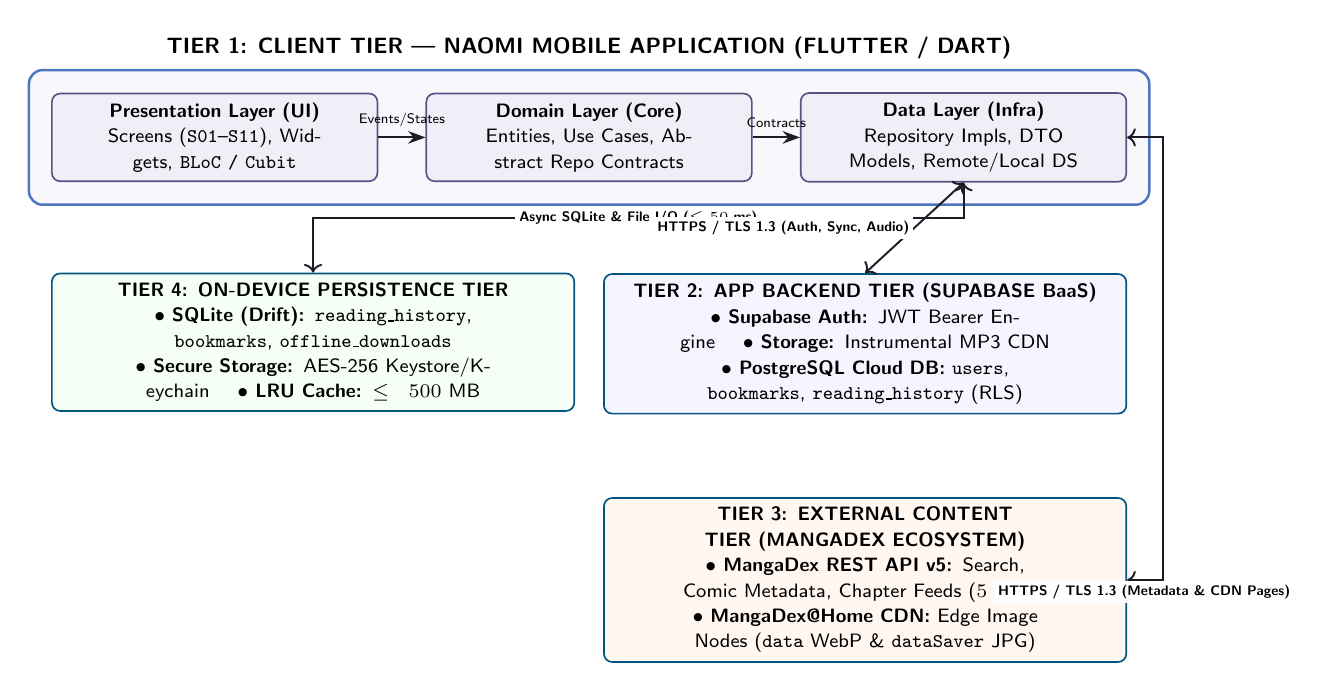
\begin{tikzpicture}[
    node distance=0.8cm and 1.0cm,
    tierbox/.style={draw=hcmutblue!70, rounded corners=5pt, line width=0.9pt, fill=naomicanvas, inner sep=8pt},
    comp/.style={draw=naomiaccent!80!black, rounded corners=3pt, fill=white, line width=0.6pt, minimum height=0.85cm, text width=3.9cm, align=center, font=\scriptsize\sffamily},
    extcomp/.style={draw=shouldblue!80!black, rounded corners=3pt, fill=white, line width=0.6pt, minimum height=0.95cm, text width=6.4cm, align=center, font=\scriptsize\sffamily},
    arr/.style={-{Stealth[length=2.2mm,width=1.6mm]}, line width=0.7pt, draw=naomidark},
    lbl/.style={font=\tiny\sffamily\bfseries, fill=white, inner sep=1.5pt}
]
    % Client Tier
    \node[comp, fill=naomitint] (ui) {\textbf{Presentation Layer (UI)}\\Screens (\texttt{S01}--\texttt{S11}), Widgets, \texttt{BLoC / Cubit}};
    \node[comp, fill=naomitint, right=0.6cm of ui] (domain) {\textbf{Domain Layer (Core)}\\Entities, Use Cases, Abstract Repo Contracts};
    \node[comp, fill=naomitint, right=0.6cm of domain] (data) {\textbf{Data Layer (Infra)}\\Repository Impls, DTO Models, Remote/Local DS};

    \begin{scope}[on background layer]
        \node[tierbox, fit=(ui)(domain)(data), label={[font=\footnotesize\sffamily\bfseries, text=black]above:TIER 1: CLIENT TIER --- NAOMI MOBILE APPLICATION (FLUTTER / DART)}] (client_tier) {};
    \end{scope}

    \draw[arr] (ui) -- node[above, font=\tiny\sffamily]{Events/States} (domain);
    \draw[arr] (domain) -- node[above, font=\tiny\sffamily]{Contracts} (data);

    % Local Tier
    \node[extcomp, below=1.15cm of ui, xshift=1.25cm, fill=green!4] (localdb) {\textbf{TIER 4: ON-DEVICE PERSISTENCE TIER}\\$\bullet$ \textbf{SQLite (Drift):} \texttt{reading\_history}, \texttt{bookmarks}, \texttt{offline\_downloads}\\$\bullet$ \textbf{Secure Storage:} AES-256 Keystore/Keychain \quad $\bullet$ \textbf{LRU Cache:} $\le 500\text{ MB}$};

    % Cloud Tier
    \node[extcomp, below=1.15cm of data, xshift=-1.25cm, fill=blue!4] (supabase) {\textbf{TIER 2: APP BACKEND TIER (SUPABASE BaaS)}\\$\bullet$ \textbf{Supabase Auth:} JWT Bearer Engine \quad $\bullet$ \textbf{Storage:} Instrumental MP3 CDN\\$\bullet$ \textbf{PostgreSQL Cloud DB:} \texttt{users}, \texttt{bookmarks}, \texttt{reading\_history} (RLS)};

    % External Tier
    \node[extcomp, below=1.05cm of supabase, fill=orange!6] (mangadex) {\textbf{TIER 3: EXTERNAL CONTENT TIER (MANGADEX ECOSYSTEM)}\\$\bullet$ \textbf{MangaDex REST API v5:} Search, Comic Metadata, Chapter Feeds ($5\text{ req/s}$)\\$\bullet$ \textbf{MangaDex@Home CDN:} Edge Image Nodes (\texttt{data} WebP \& \texttt{dataSaver} JPG)};

    \draw[arr, <->] (data.south) -- ++(0,-0.45) -| node[pos=0.25, lbl]{Async SQLite \& File I/O ($\le 50\text{ ms}$)} (localdb.north);
    \draw[arr, <->] (data.south) -- node[left, lbl]{HTTPS / TLS 1.3 (Auth, Sync, Audio)} (supabase.north);
    \draw[arr, <->] (data.east) -- ++(0.45,0) |- node[pos=0.76, below, lbl]{HTTPS / TLS 1.3 (Metadata \& CDN Pages)} (mangadex.east);
\end{tikzpicture}
\caption{C4 Container \& Multi-Tier System Architecture Diagram of the Naomi Ecosystem.}
\label{fig:c4_architecture}
\end{figure}

\subsection{In-App Clean Architecture \& BLoC State Management}
\label{subsec:in_app_arch}

To satisfy Rubric Criterion 1.4 and 2.2 (\textit{``Follows the designed architecture, clear layering, sound state management''}), the internal mobile codebase enforces Uncle Bob's \textbf{Clean Architecture} combined with the unidirectional \textbf{BLoC (Business Logic Component)} pattern (Figure~\ref{fig:clean_arch}):

\begin{itemize}
    \item \textbf{Presentation Layer (\texttt{lib/presentation/}):} Contains declarative Flutter Screens (\texttt{S01}--\texttt{S11}), reusable UI widgets, and \texttt{BLoC}/\texttt{Cubit} state controllers (\texttt{AuthBloc}, \texttt{HomeBloc}, \texttt{DiscoverBloc}, \texttt{Comic\allowbreak Detail\allowbreak Bloc}, \texttt{ReaderBloc}, \texttt{AudioCubit}, \texttt{DownloadBloc}, \texttt{LibraryBloc}, \texttt{SettingsCubit}, \texttt{Connectivity\allowbreak Cubit}). UI widgets never invoke network or database APIs directly; they only dispatch immutable \texttt{Events} and rebuild reactively on emitted \texttt{States} (\texttt{Initial}, \texttt{Loading}, \texttt{Loaded}, \texttt{Empty}, \texttt{Error}).
    \item \textbf{Domain Layer (\texttt{lib/domain/} -- Pure Dart Core):} Houses immutable business \texttt{Entities} (\texttt{ComicEntity}, \texttt{ChapterEntity}, \texttt{PageEntity}, \texttt{AmbientTrackEntity}, \texttt{UserProfile\allowbreak Entity}), single-responsibility \texttt{UseCases} (\texttt{SignInUseCase}, \texttt{Search\allowbreak Comics\allowbreak UseCase}, \texttt{Get\allowbreak Chapter\allowbreak Content\allowbreak UseCase}, \texttt{Save\allowbreak Reading\allowbreak Progress\allowbreak UseCase}, \texttt{Get\allowbreak Genre\allowbreak Audio\allowbreak UseCase}), and abstract \texttt{Repository Interfaces} (\texttt{IComicRepository}, \texttt{IAuthRepository}). In strict compliance with \textbf{The Dependency Rule}, the Domain layer has zero imports from Flutter UI, \texttt{dio}, \texttt{drift}, or \texttt{supabase\_flutter}.
    \item \textbf{Data Layer (\texttt{lib/data/} -- Infrastructure):} Implements the domain contracts (\texttt{Comic\allowbreak Repository\allowbreak Impl}, \texttt{Auth\allowbreak Repository\allowbreak Impl}), serialises JSON/SQLite \texttt{DTO Models}, and orchestrates Remote Data Sources (\texttt{Manga\allowbreak Dex\allowbreak Api\allowbreak Client}, \texttt{Supabase\allowbreak Api\allowbreak Client}) alongside Local Data Sources (\texttt{Drift\allowbreak App\allowbreak Database}, \texttt{Secure\allowbreak Storage\allowbreak Manager}, \texttt{Local\allowbreak File\allowbreak Storage}).
\end{itemize}

\begin{figure}[H]
\centering
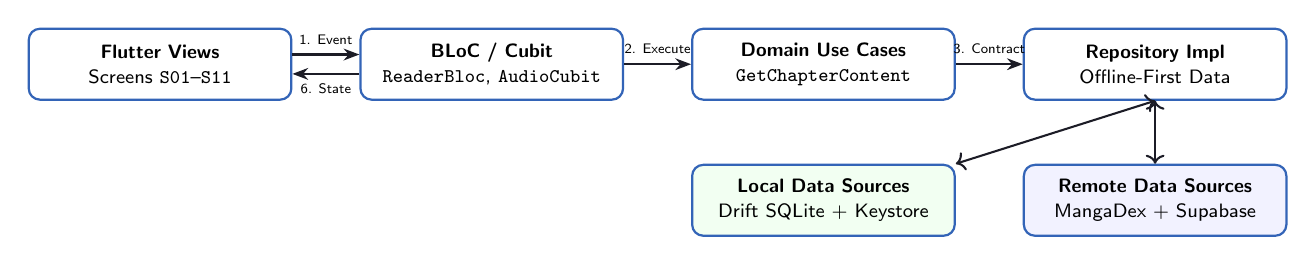
\begin{tikzpicture}[
    box/.style={draw=hcmutblue!80, rounded corners=4pt, fill=white, line width=0.8pt, minimum height=0.9cm, text width=3.1cm, align=center, font=\scriptsize\sffamily},
    layer/.style={draw=naomiaccent, rounded corners=5pt, line width=0.9pt, fill=naomitint!50, inner sep=7pt},
    arr/.style={-{Stealth[length=2.0mm,width=1.5mm]}, line width=0.75pt, draw=naomidark}
]
    \node[box] (view) {\textbf{Flutter Views}\\Screens \texttt{S01}--\texttt{S11}};
    \node[box, right=0.85cm of view] (bloc) {\textbf{BLoC / Cubit}\\\texttt{ReaderBloc}, \texttt{AudioCubit}};
    \node[box, right=0.85cm of bloc] (uc) {\textbf{Domain Use Cases}\\\texttt{GetChapterContent}};
    \node[box, right=0.85cm of uc] (repo) {\textbf{Repository Impl}\\Offline-First Data};

    \node[box, below=0.8cm of uc, fill=green!5] (local) {\textbf{Local Data Sources}\\Drift SQLite + Keystore};
    \node[box, below=0.8cm of repo, fill=blue!5] (remote) {\textbf{Remote Data Sources}\\MangaDex + Supabase};

    \draw[arr, transform canvas={yshift=3.5pt}] (view) -- node[above, font=\tiny\sffamily]{1. Event} (bloc);
    \draw[arr, transform canvas={yshift=-3.5pt}] (bloc) -- node[below, font=\tiny\sffamily]{6. State} (view);
    \draw[arr] (bloc) -- node[above, font=\tiny\sffamily]{2. Execute} (uc);
    \draw[arr] (uc) -- node[above, font=\tiny\sffamily]{3. Contract} (repo);
    \draw[arr, <->] (repo.south) -- (local.north east);
    \draw[arr, <->] (repo.south) -- (remote.north);
\end{tikzpicture}
\caption{Unidirectional data and state flow across Clean Architecture layers (\texttt{UI} $\leftrightarrow$ \texttt{BLoC} $\leftrightarrow$ \texttt{UseCase} $\leftrightarrow$ \texttt{Repository}).}
\label{fig:clean_arch}
\end{figure}

\subsection{UML Sequence Diagrams for Core System Flows}
\label{subsec:sequence_diagrams}

Figures~\ref{fig:seq_reader}, \ref{fig:seq_download}, and \ref{fig:seq_auth} model the exact runtime message choreography across architectural components for the three primary operational flows of \textbf{Naomi}.

\subsubsection{Flow 1: Full-Screen Preloaded Reading with Genre Ambient Audio (UC-03, UC-04, UC-05)}
\begin{figure}[H]
\centering
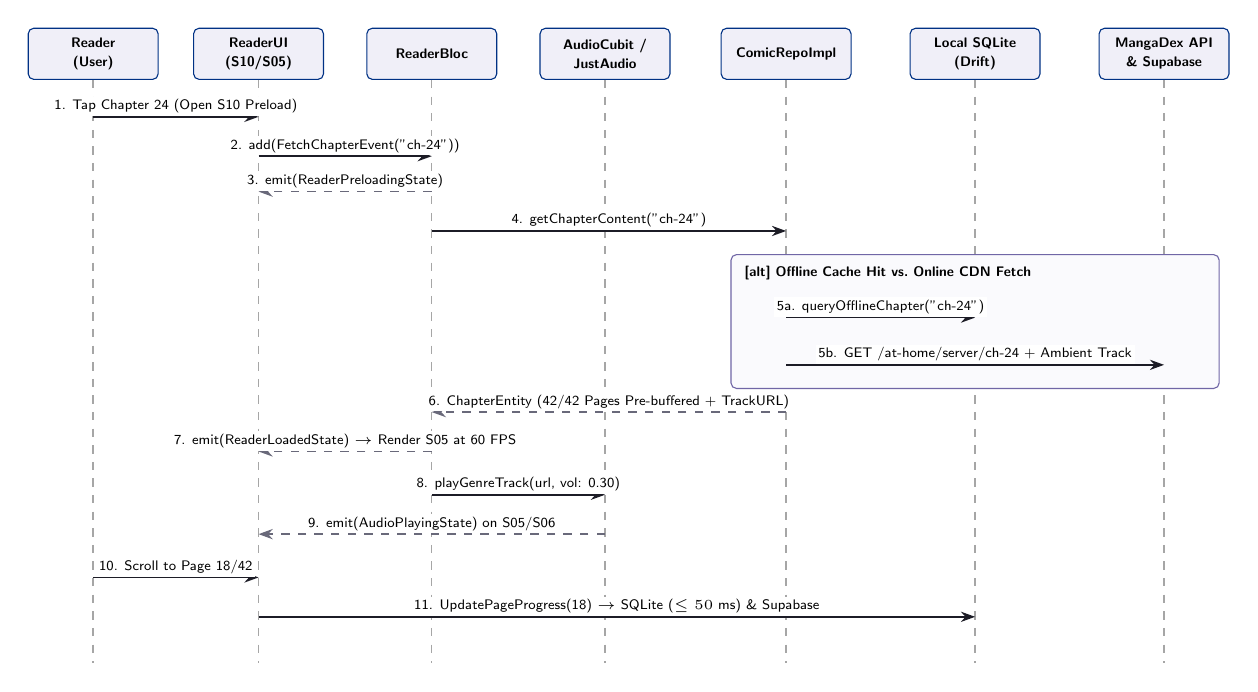
\begin{tikzpicture}[
    lifeline/.style={draw=hcmutblue!80!black, fill=naomitint, rounded corners=2pt, font=\tiny\sffamily\bfseries, minimum height=0.65cm, minimum width=1.65cm, align=center},
    msg/.style={-{Stealth[length=1.8mm,width=1.3mm]}, line width=0.6pt, draw=naomidark},
    ret/.style={-{Stealth[length=1.8mm,width=1.3mm]}, line width=0.6pt, dashed, draw=naomimuted!90!black},
    lbl/.style={font=\tiny\sffamily, inner sep=1pt, fill=white}
]
    \node[lifeline] (p0) at (0,0) {Reader\\(User)};
    \node[lifeline] (p1) at (2.1,0) {ReaderUI\\(S10/S05)};
    \node[lifeline] (p2) at (4.3,0) {ReaderBloc};
    \node[lifeline] (p3) at (6.5,0) {AudioCubit /\\JustAudio};
    \node[lifeline] (p4) at (8.8,0) {ComicRepoImpl};
    \node[lifeline] (p5) at (11.2,0) {Local SQLite\\(Drift)};
    \node[lifeline] (p6) at (13.6,0) {MangaDex API\\\& Supabase};

    \foreach \i in {0,...,6} {
        \draw[dashed, gray!70, line width=0.5pt] (p\i.south) -- ++(0,-7.4);
    }

    \draw[msg] (0,-0.8) -- node[above, lbl]{1. Tap Chapter 24 (Open S10 Preload)} (2.1,-0.8);
    \draw[msg] (2.1,-1.3) -- node[above, lbl]{2. add(FetchChapterEvent("ch-24"))} (4.3,-1.3);
    \draw[ret] (4.3,-1.75) -- node[above, lbl]{3. emit(ReaderPreloadingState)} (2.1,-1.75);
    \draw[msg] (4.3,-2.25) -- node[above, lbl]{4. getChapterContent("ch-24")} (8.8,-2.25);

    \draw[rounded corners=2pt, draw=naomiaccent, fill=naomitint!30] (8.1,-2.55) rectangle (14.3,-4.25);
    \node[font=\tiny\sffamily\bfseries, anchor=north west, text=black] at (8.15,-2.57) {[alt] Offline Cache Hit vs.\ Online CDN Fetch};
    \draw[msg] (8.8,-3.35) -- node[above, lbl]{5a. queryOfflineChapter("ch-24")} (11.2,-3.35);
    \draw[msg] (8.8,-3.95) -- node[above, lbl]{5b. GET /at-home/server/ch-24 + Ambient Track} (13.6,-3.95);

    \draw[ret] (8.8,-4.55) -- node[above, lbl]{6. ChapterEntity (42/42 Pages Pre-buffered + TrackURL)} (4.3,-4.55);
    \draw[ret] (4.3,-5.05) -- node[above, lbl]{7. emit(ReaderLoadedState) $\to$ Render S05 at 60 FPS} (2.1,-5.05);
    \draw[msg] (4.3,-5.6) -- node[above, lbl]{8. playGenreTrack(url, vol: 0.30)} (6.5,-5.6);
    \draw[ret] (6.5,-6.1) -- node[above, lbl]{9. emit(AudioPlayingState) on S05/S06} (2.1,-6.1);

    \draw[msg] (0,-6.65) -- node[above, lbl]{10. Scroll to Page 18/42} (2.1,-6.65);
    \draw[msg] (2.1,-7.15) -- node[above, lbl]{11. UpdatePageProgress(18) $\to$ SQLite ($\le 50\text{ ms}$) \& Supabase} (11.2,-7.15);
\end{tikzpicture}
\caption{UML Sequence Diagram for Flow 1: Full-Chapter Preload (\texttt{S10}), 60 FPS Reading (\texttt{S05}), Genre Ambient Audio (\texttt{S06}), and Page Progress Sync.}
\label{fig:seq_reader}
\end{figure}

\subsubsection{Flow 2: Offline Chapter Download \& Sandboxed Persistence (UC-06)}
\begin{figure}[H]
\centering
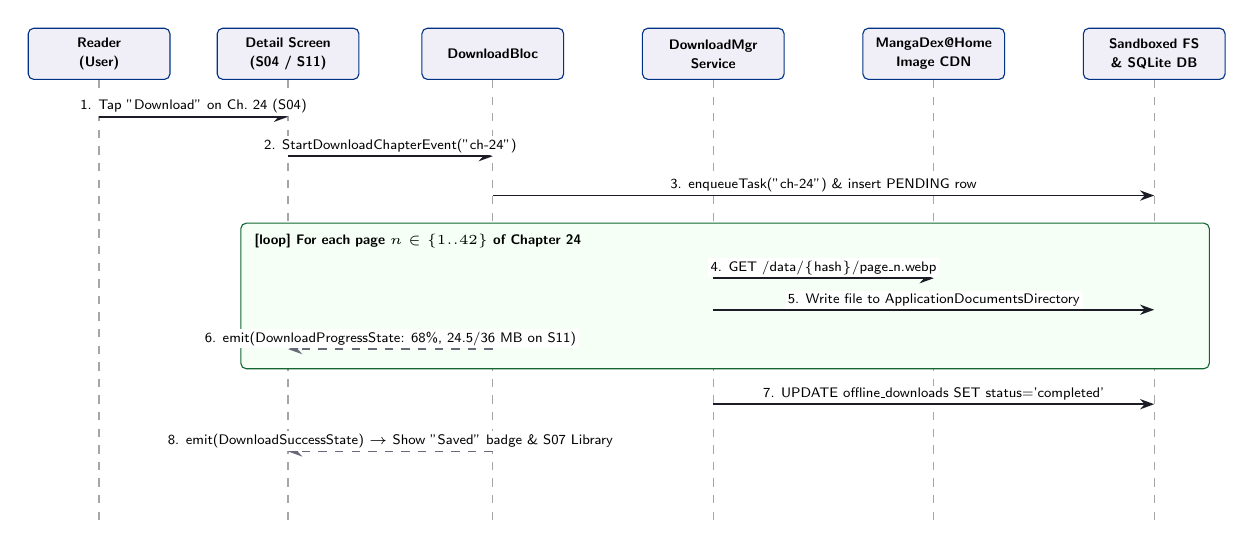
\begin{tikzpicture}[
    lifeline/.style={draw=hcmutblue!80!black, fill=naomitint, rounded corners=2pt, font=\tiny\sffamily\bfseries, minimum height=0.65cm, minimum width=1.8cm, align=center},
    msg/.style={-{Stealth[length=1.8mm,width=1.3mm]}, line width=0.6pt, draw=naomidark},
    ret/.style={-{Stealth[length=1.8mm,width=1.3mm]}, line width=0.6pt, dashed, draw=naomimuted!90!black},
    lbl/.style={font=\tiny\sffamily, inner sep=1pt, fill=white}
]
    \node[lifeline] (d0) at (0,0) {Reader\\(User)};
    \node[lifeline] (d1) at (2.4,0) {Detail Screen\\(S04 / S11)};
    \node[lifeline] (d2) at (5.0,0) {DownloadBloc};
    \node[lifeline] (d3) at (7.8,0) {DownloadMgr\\Service};
    \node[lifeline] (d4) at (10.6,0) {MangaDex@Home\\Image CDN};
    \node[lifeline] (d5) at (13.4,0) {Sandboxed FS\\\& SQLite DB};

    \foreach \i in {0,...,5} {
        \draw[dashed, gray!70, line width=0.5pt] (d\i.south) -- ++(0,-5.6);
    }

    \draw[msg] (0,-0.8) -- node[above, lbl]{1. Tap "Download" on Ch.\ 24 (S04)} (2.4,-0.8);
    \draw[msg] (2.4,-1.3) -- node[above, lbl]{2. StartDownloadChapterEvent("ch-24")} (5.0,-1.3);
    \draw[msg] (5.0,-1.8) -- node[above, lbl]{3. enqueueTask("ch-24") \& insert PENDING row} (13.4,-1.8);

    \draw[rounded corners=2pt, draw=mustgreen!80!black, fill=green!4] (1.8,-2.15) rectangle (14.1,-4.0);
    \node[font=\tiny\sffamily\bfseries, anchor=north west, text=black] at (1.85,-2.17) {[loop] For each page $n \in \{1..42\}$ of Chapter 24};
    \draw[msg] (7.8,-2.85) -- node[above, lbl]{4. GET /data/\{hash\}/page\_n.webp} (10.6,-2.85);
    \draw[msg] (7.8,-3.25) -- node[above, lbl]{5. Write file to ApplicationDocumentsDirectory} (13.4,-3.25);
    \draw[ret] (5.0,-3.75) -- node[above, lbl]{6. emit(DownloadProgressState: 68\%, 24.5/36 MB on S11)} (2.4,-3.75);

    \draw[msg] (7.8,-4.45) -- node[above, lbl]{7. UPDATE offline\_downloads SET status='completed'} (13.4,-4.45);
    \draw[ret] (5.0,-5.05) -- node[above, lbl]{8. emit(DownloadSuccessState) $\to$ Show "Saved" badge \& S07 Library} (2.4,-5.05);
\end{tikzpicture}
\caption{UML Sequence Diagram for Flow 2: Sequential Chapter Page Download (\texttt{S11}) and Local SQLite Registration.}
\label{fig:seq_download}
\end{figure}

\subsubsection{Flow 3: User Authentication \& Hardware-Backed Auto-Login (UC-00)}
\begin{figure}[H]
\centering
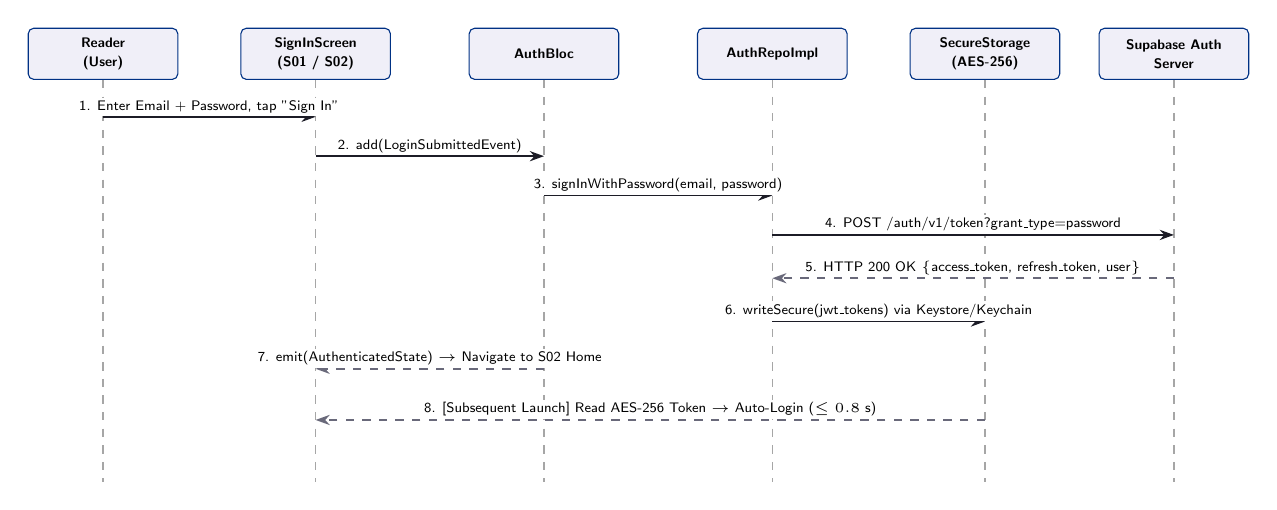
\begin{tikzpicture}[
    lifeline/.style={draw=hcmutblue!80!black, fill=naomitint, rounded corners=2pt, font=\tiny\sffamily\bfseries, minimum height=0.65cm, minimum width=1.9cm, align=center},
    msg/.style={-{Stealth[length=1.8mm,width=1.3mm]}, line width=0.6pt, draw=naomidark},
    ret/.style={-{Stealth[length=1.8mm,width=1.3mm]}, line width=0.6pt, dashed, draw=naomimuted!90!black},
    lbl/.style={font=\tiny\sffamily, inner sep=1pt, fill=white}
]
    \node[lifeline] (a0) at (0,0) {Reader\\(User)};
    \node[lifeline] (a1) at (2.7,0) {SignInScreen\\(S01 / S02)};
    \node[lifeline] (a2) at (5.6,0) {AuthBloc};
    \node[lifeline] (a3) at (8.5,0) {AuthRepoImpl};
    \node[lifeline] (a4) at (11.2,0) {SecureStorage\\(AES-256)};
    \node[lifeline] (a5) at (13.6,0) {Supabase Auth\\Server};

    \foreach \i in {0,...,5} {
        \draw[dashed, gray!70, line width=0.5pt] (a\i.south) -- ++(0,-5.1);
    }

    \draw[msg] (0,-0.8) -- node[above, lbl]{1. Enter Email + Password, tap "Sign In"} (2.7,-0.8);
    \draw[msg] (2.7,-1.3) -- node[above, lbl]{2. add(LoginSubmittedEvent)} (5.6,-1.3);
    \draw[msg] (5.6,-1.8) -- node[above, lbl]{3. signInWithPassword(email, password)} (8.5,-1.8);
    \draw[msg] (8.5,-2.3) -- node[above, lbl]{4. POST /auth/v1/token?grant\_type=password} (13.6,-2.3);
    \draw[ret] (13.6,-2.85) -- node[above, lbl]{5. HTTP 200 OK \{access\_token, refresh\_token, user\}} (8.5,-2.85);
    \draw[msg] (8.5,-3.4) -- node[above, lbl]{6. writeSecure(jwt\_tokens) via Keystore/Keychain} (11.2,-3.4);
    \draw[ret] (5.6,-4.0) -- node[above, lbl]{7. emit(AuthenticatedState) $\to$ Navigate to S02 Home} (2.7,-4.0);
    \draw[ret] (11.2,-4.65) -- node[above, lbl]{8. [Subsequent Launch] Read AES-256 Token $\to$ Auto-Login ($\le 0.8\text{ s}$)} (2.7,-4.65);
\end{tikzpicture}
\caption{UML Sequence Diagram for Flow 3: Supabase JWT Authentication (\texttt{S01}) and Hardware-Backed Keystore Persistence.}
\label{fig:seq_auth}
\end{figure}

\subsection{Justified Technology Choices}
\label{subsec:tech_justification}

To fulfil Rubric Criterion 1.4 (\textit{``justified technology choices''}), Table~\ref{tab:tech_justification} presents a rigorous comparative trade-off evaluation across the four foundational architectural decisions of \textbf{Naomi}.

\begin{table}[H]
\centering
\caption{Comparative architectural trade-off analysis and justification of selected technologies.}
\label{tab:tech_justification}
\footnotesize
\renewcommand{\arraystretch}{1.26}
\begin{tabularx}{\textwidth}{L{2.8cm} L{3.4cm} L{3.3cm} Y}
\toprule
\rowcolor{tablehead}
\textbf{Architectural Layer} & \textbf{Selected Technology} & \textbf{Evaluated Alternatives} & \textbf{Technical Rationale \& Mobile Engineering Justification} \\
\midrule
\textbf{Cross-Platform Mobile Framework} & \textbf{Flutter 3.x (Dart, Impeller / Skia)} & React Native (JS Bridge), Native Kotlin / Swift & \textbf{Eliminates bridge bottlenecks during Webtoon scrolling:} Flutter compiles AOT to native ARM64 code and renders every pixel directly onto its own Impeller/Skia GPU canvas, sustaining $\ge 60\text{ FPS}$ (\texttt{NFR-03}) across 50-page vertical strips while halving development effort compared to dual Kotlin/Swift codebases. \\
\rowcolor{tablerow}
\textbf{In-App Architecture \& State Management} & \textbf{Clean Architecture + \texttt{flutter\_bloc}} & MVC / Basic MVVM, Vanilla \texttt{Provider} / \texttt{setState} & \textbf{Strict separation of concerns \& deterministic unit testing:} Unidirectional \texttt{Event $\to$ BLoC $\to$ State} streams prevent ``Fat Widget/Controller'' anti-patterns and allow $100\%$ isolated unit testing of domain use cases and BLoC transitions in Assignment 02 via \texttt{bloc\_test}. \\
\textbf{Cloud Backend \& Auth Platform} & \textbf{Supabase BaaS (PostgreSQL + Auth + Storage)} & Custom Node.js/Express + MongoDB, Firebase & \textbf{Relational integrity + zero-downtime cloud infrastructure:} Unlike NoSQL Firestore/MongoDB, Supabase provides a true \textbf{PostgreSQL} engine enforcing 3NF/BCNF foreign keys and database-level \textbf{Row-Level Security (RLS)}, paired with built-in JWT Auth and CDN Buckets for streaming MP3 ambient audio. \\
\rowcolor{tablerow}
\textbf{On-Device Local Database} & \textbf{SQLite via \texttt{Drift} (Type-Safe ORM)} & \texttt{SharedPreferences}, NoSQL \texttt{Hive} & \textbf{Relational hierarchy \& sub-50 ms indexed queries:} Comic data is inherently relational (\texttt{comics} $1\text{:}N$ \texttt{chapters} $1\text{:}N$ \texttt{pages}). SQLite supports foreign-key \texttt{ON DELETE CASCADE} and composite indexes on \texttt{(user\_id, chapter\_id)}, achieving $\le 50\text{ ms}$ query times (\texttt{NFR-09}) without blocking the UI thread. \\
\bottomrule
\end{tabularx}
\end{table}

\newpage
\section{Data \& API Design}
\label{sec:data_api}

\subsection{Hybrid Offline-First Data Architecture \& Data Dictionary}
\label{subsec:data_dictionary}

The data persistence layer of \textbf{Naomi} follows a \textbf{Hybrid Offline-First} paradigm spanning three synchronised storage domains: (1) \textbf{Supabase Cloud PostgreSQL} as the single source of truth for user identity, cloud bookmarks, reading history, and genre-audio mappings; (2) \textbf{MangaDex REST API v5 \& MangaDex@Home CDN} as the global comic metadata and page-image provider; and (3) \textbf{On-Device SQLite (Drift) + Sandboxed File Storage} for instant local reads and full offline operation. Table~\ref{tab:data_dictionary} summarises the 10 normalised relational tables.

\begin{table}[H]
\centering
\caption{System Data Dictionary across the 10 normalised tables of the Naomi database schema.}
\label{tab:data_dictionary}
\footnotesize
\renewcommand{\arraystretch}{1.22}
\begin{tabularx}{\textwidth}{C{0.7cm} L{3.1cm} L{2.8cm} Y C{2.2cm}}
\toprule
\rowcolor{tablehead}
\textbf{\#} & \textbf{Table Name} & \textbf{Storage Location} & \textbf{Primary Purpose \& Entity Role} & \textbf{FR Mapping} \\
\midrule
1 & \texttt{users} & Supabase Cloud & User profile linked 1:1 to \texttt{auth.users(id)}, display name, avatar, and JSONB UI preferences. & \texttt{FR-00, FR-14} \\
\rowcolor{tablerow}
2 & \texttt{comics} & Cloud \& Local Cache & Comic series metadata (title, alt\_title, author, artist, status, cover\_url, default ambient track). & \texttt{FR-01, FR-08, FR-10} \\
3 & \texttt{genres} & Cloud \& Local Cache & Canonical genre catalogue (\texttt{action, fantasy, romance, slice\_of\_life}, etc.). & \texttt{FR-01, FR-05} \\
\rowcolor{tablerow}
4 & \texttt{comic\_genres} & Cloud \& Local Cache & Associative $M\text{:}N$ join table linking \texttt{comics} and \texttt{genres} via composite PK. & \texttt{FR-01, FR-05} \\
5 & \texttt{chapters} & Cloud \& Local Cache & Individual chapter metadata (chapter\_number, volume, title, page\_count, optional audio override). & \texttt{FR-02, FR-04, FR-10} \\
\rowcolor{tablerow}
6 & \texttt{pages} & Cloud \& Local Cache & \textbf{Weak Entity} representing ordered pages within a chapter, identified by \texttt{(chapter\_id, page\_number)}. & \texttt{FR-02, FR-03} \\
7 & \texttt{ambient\_tracks} & Supabase DB/Storage & Instrumental background tracks categorised by genre with streaming MP3 URLs and loop metadata. & \texttt{FR-05, FR-09} \\
\rowcolor{tablerow}
8 & \texttt{reading\_history} & Cloud \& Local SQLite & Exact page-level progress (\texttt{last\_page\_read}, \texttt{read\_percentage}, \texttt{is\_synced}); strictly 3NF. & \texttt{FR-04, FR-08} \\
9 & \texttt{bookmarks} & Cloud \& Local SQLite & User's personal bookmarked series (\texttt{is\_favorite}, \texttt{reading\_status}) synced across devices. & \texttt{FR-07, FR-10} \\
\rowcolor{tablerow}
10 & \texttt{offline\_downloads} & Local SQLite Only & Tracks local chapter download status, byte size, and relative directory path in sandboxed storage; strictly 3NF. & \texttt{FR-06, FR-07, FR-13} \\
\bottomrule
\end{tabularx}
\end{table}

\subsection{Conceptual \& Physical Entity-Relationship Diagrams}
\label{subsec:erd_diagrams}

Following standard database design methodology (\textit{Elmasri \& Navathe, Fundamentals of Database Systems, 7th Ed., Chapters 2--3}), Figure~\ref{fig:erd_chen} presents the \textbf{Conceptual Entity-Relationship Diagram in Chen Notation} (highlighting strong vs.\ weak entities, identifying relationships, total participation double lines, and partial key dashed underlines), while Figure~\ref{fig:erd_crowsfoot} presents the mapped \textbf{Physical Relational Schema in Crow's Foot Notation}.

\begin{figure}[H]
    \centering
    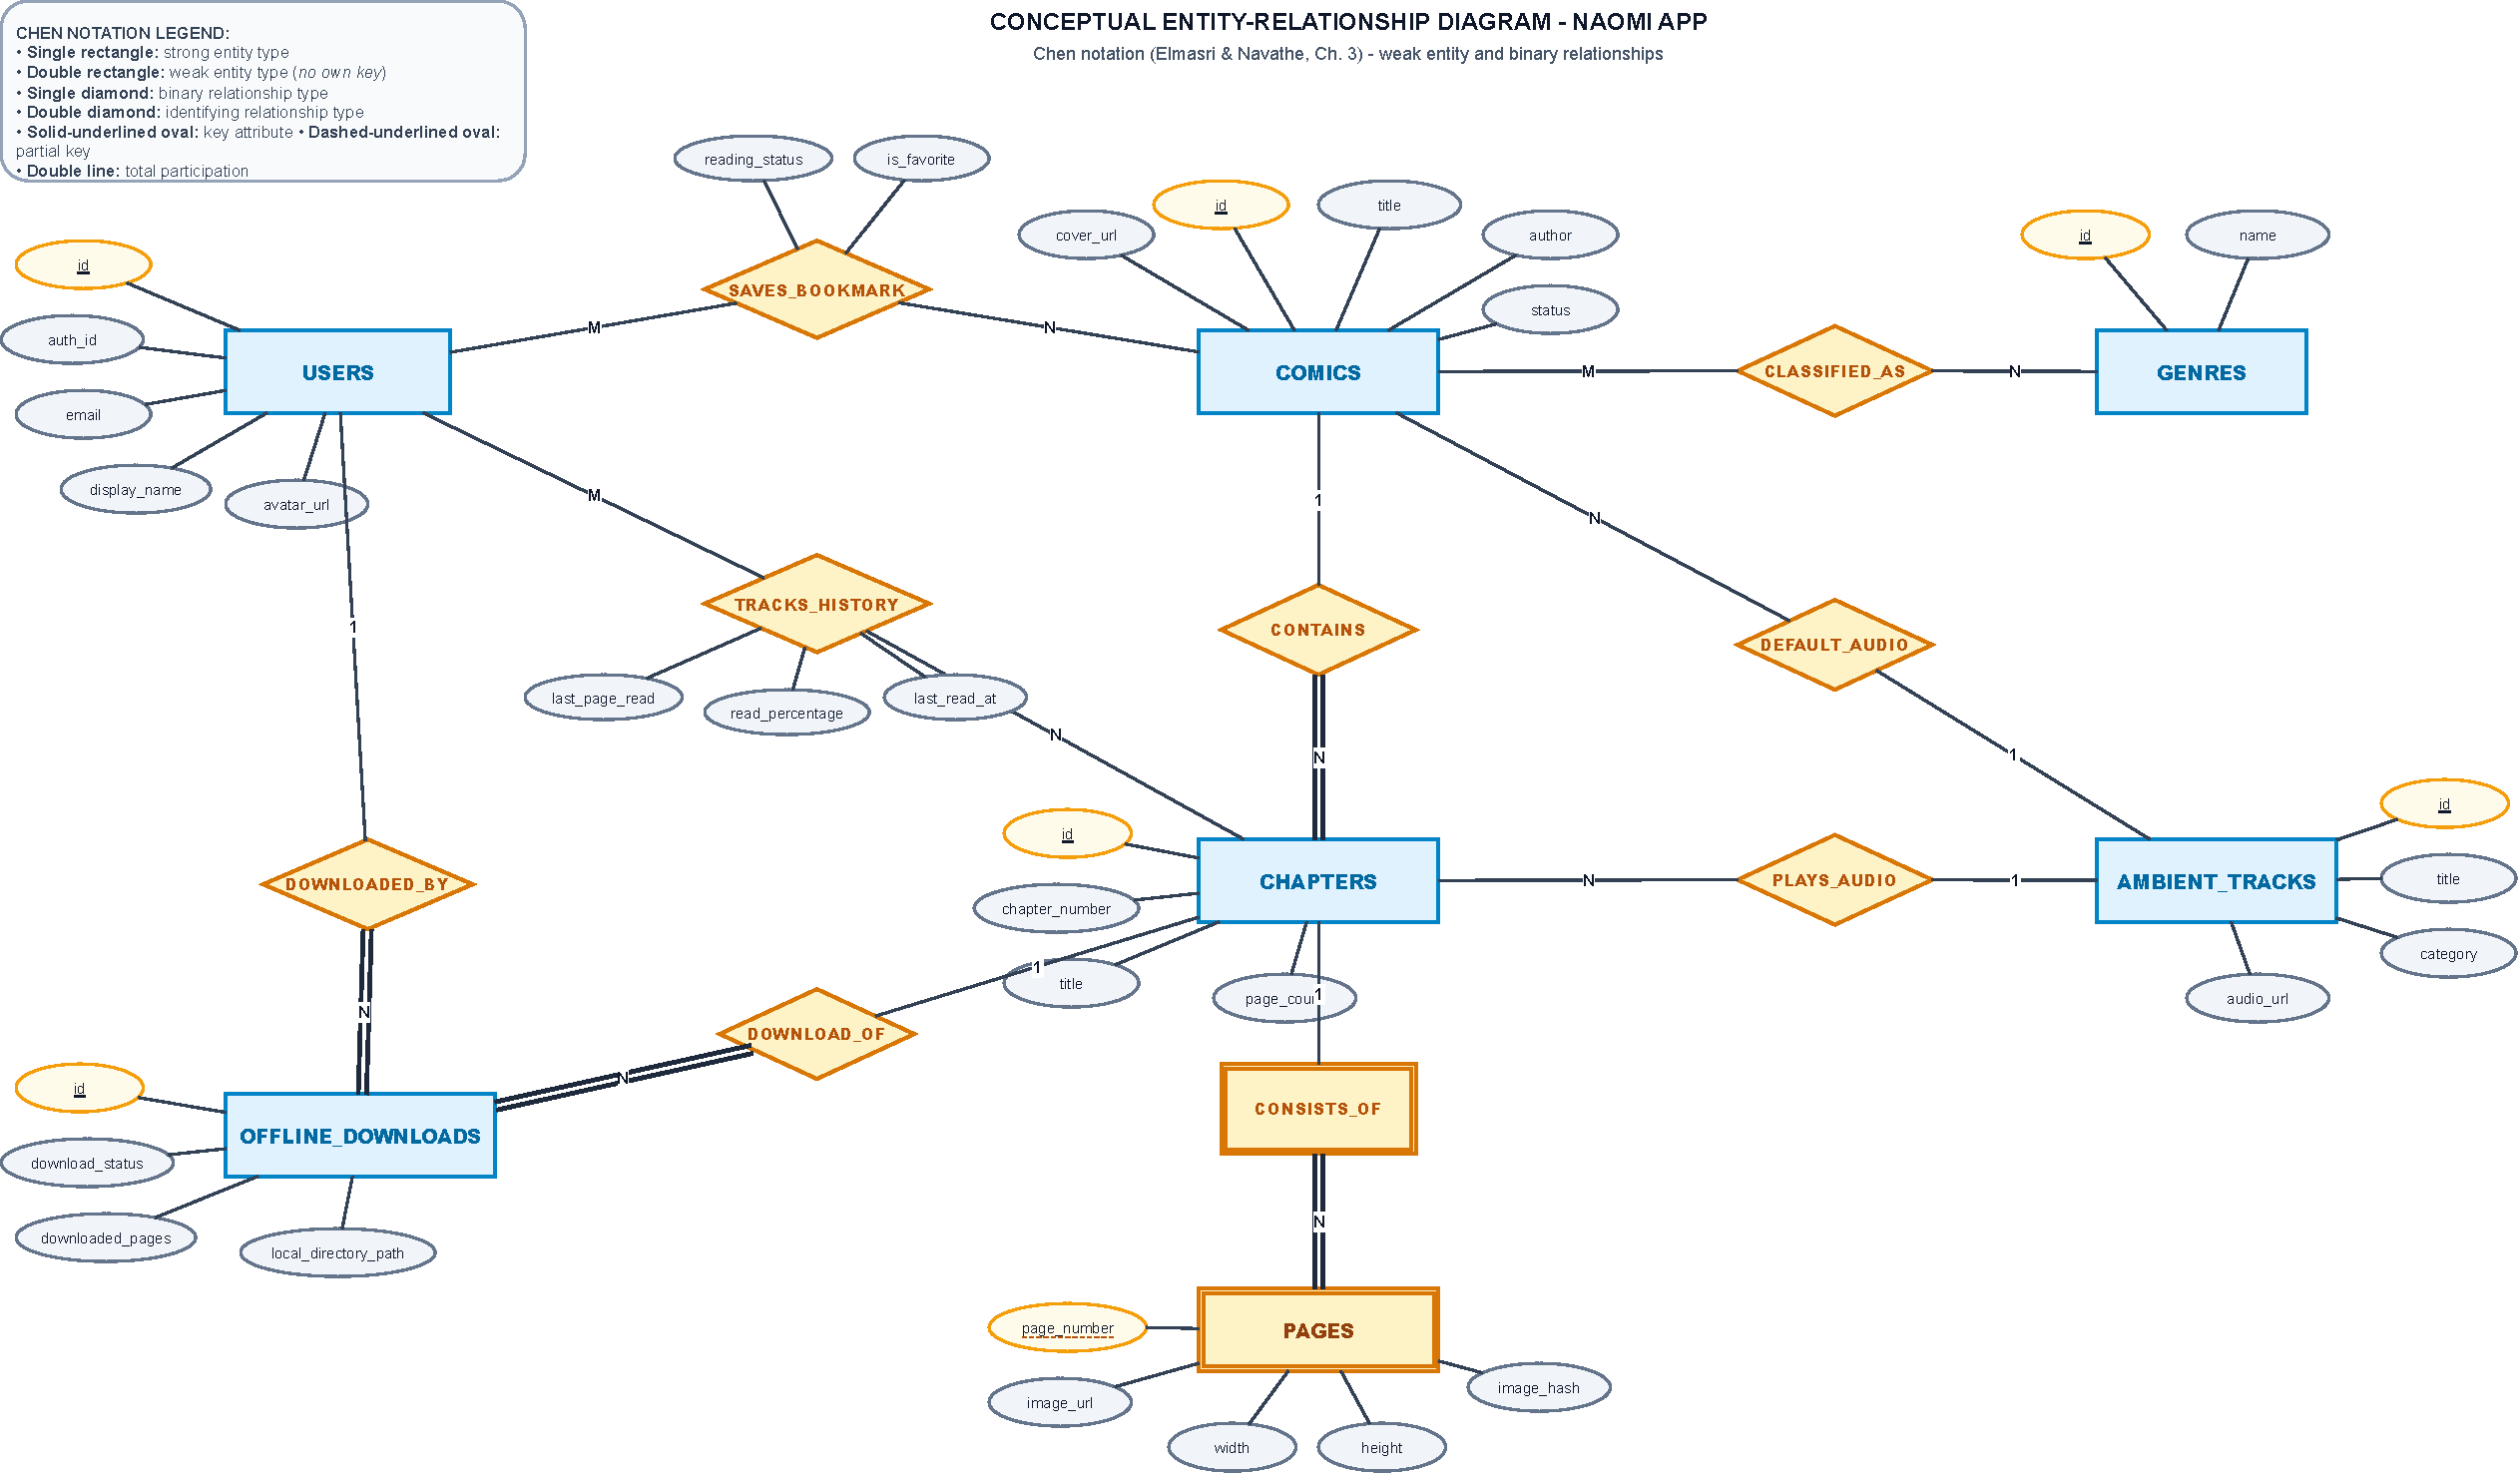
\includegraphics[width=0.99\textwidth]{figures/diagrams/erd_conceptual_chen.pdf}
    \caption{Conceptual Entity-Relationship Diagram (Chen Notation) illustrating strong entities, the weak entity \texttt{PAGES} with partial key \texttt{page\_number}, and binary relationships.}
    \label{fig:erd_chen}
\end{figure}

\begin{figure}[H]
    \centering
    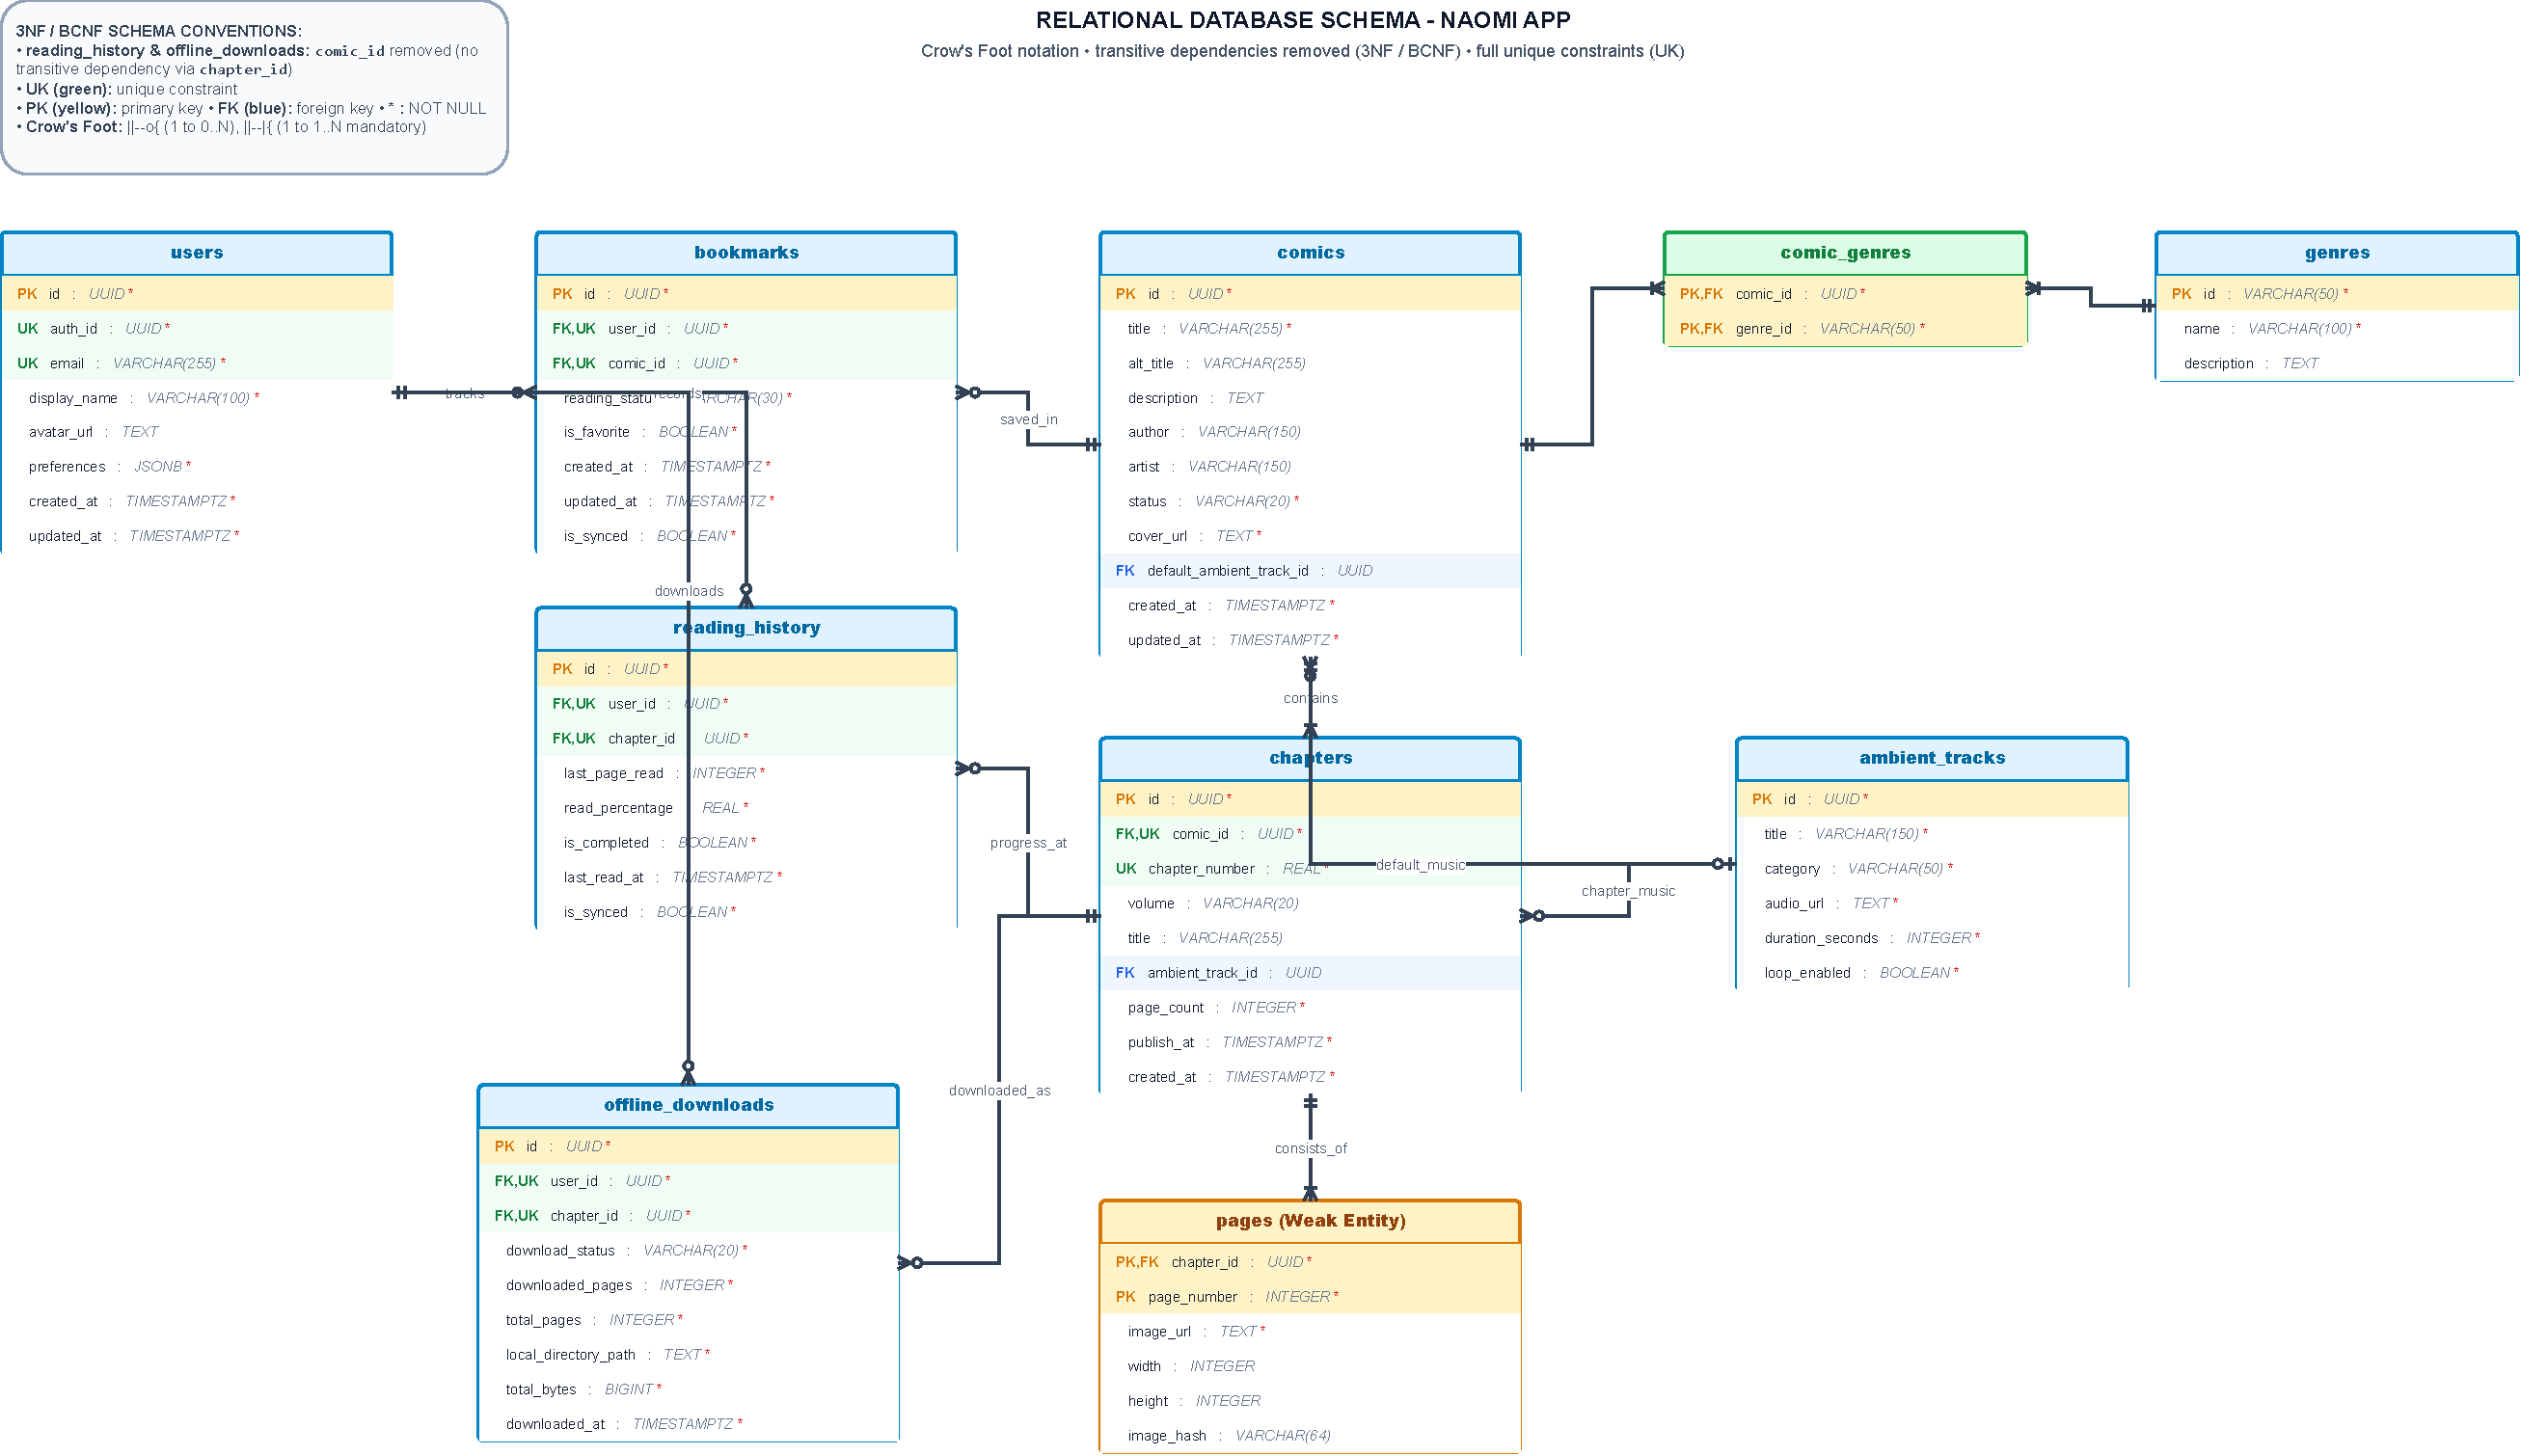
\includegraphics[width=0.99\textwidth]{figures/diagrams/erd_relational_crowsfoot.pdf}
    \caption{Physical Relational Database Schema (Crow's Foot Notation) enforcing 3NF/BCNF, Primary Keys (PK), Foreign Keys (FK), and Unique Constraints (UK).}
    \label{fig:erd_crowsfoot}
\end{figure}

\subsection{Detailed Relational Schema, 3NF/BCNF Normalisation Proof \& RLS Security}
\label{subsec:schema_norm_rls}

\subsubsection{Relational Schema Specifications (10 Tables)}
\begin{itemize}
    \item \textbf{\texttt{users}:} \texttt{id UUID PK}, \texttt{auth\_id UUID UNIQUE NOT NULL}, \texttt{email VARCHAR(255) UNIQUE NOT NULL}, \texttt{display\_name VARCHAR(100) NOT NULL}, \texttt{avatar\_url TEXT}, \texttt{preferences JSONB DEFAULT} \allowbreak \texttt{'\{"scroll\_direction":} \allowbreak \texttt{"vertical",} \allowbreak \texttt{"ambient\_auto\_play":} \allowbreak \texttt{true,} \allowbreak \texttt{"ambient\_volume":0.3\}'}, \texttt{created\_at TIMESTAMPTZ}, \texttt{updated\_at TIMESTAMPTZ}.
    \item \textbf{\texttt{comics}:} \texttt{id UUID PK}, \texttt{title VARCHAR(255) NOT NULL}, \texttt{alt\_title VARCHAR(255)}, \texttt{description TEXT}, \texttt{author VARCHAR(150)}, \texttt{artist VARCHAR(150)}, \texttt{status VARCHAR(20) CHECK (status IN ('ongoing','completed','hiatus','cancelled'))}, \texttt{cover\_url TEXT NOT NULL}, \texttt{default\_ambient\_track\_id UUID} \allowbreak \texttt{FK $\to$ ambient\_tracks(id) ON DELETE SET NULL}, \texttt{created\_at}, \texttt{updated\_at}.
    \item \textbf{\texttt{genres} \& \texttt{comic\_genres}:} \texttt{genres(id VARCHAR(50) PK, name VARCHAR(100) NOT NULL, description TEXT)}; \texttt{comic\_genres(comic\_id UUID FK, genre\_id VARCHAR(50) FK,} \allowbreak \texttt{PRIMARY KEY (comic\_id, genre\_id))}.
    \item \textbf{\texttt{chapters}:} \texttt{id UUID PK}, \texttt{comic\_id UUID NOT NULL FK $\to$ comics(id) ON DELETE CASCADE}, \texttt{chapter\_number REAL NOT NULL}, \texttt{volume VARCHAR(20)}, \texttt{title VARCHAR(255)}, \texttt{ambient\_track\_id UUID FK $\to$ ambient\_tracks(id) ON DELETE SET NULL}, \texttt{page\_count INT NOT NULL}, \texttt{publish\_at TIMESTAMPTZ}, \texttt{created\_at TIMESTAMPTZ}, with \texttt{UNIQUE(comic\_id, chapter\_number)}.
    \item \textbf{\texttt{pages} (Weak Entity Mapping):} \texttt{chapter\_id UUID NOT NULL FK $\to$ chapters(id) ON DELETE CASCADE}, \texttt{page\_number INT NOT NULL}, \texttt{image\_url TEXT NOT NULL}, \texttt{width INT}, \texttt{height INT}, \texttt{image\_hash VARCHAR(64)}, with composite \texttt{PRIMARY KEY} \allowbreak \texttt{(chapter\_id, page\_number)}.
    \item \textbf{\texttt{ambient\_tracks}:} \texttt{id UUID PK}, \texttt{title VARCHAR(150) NOT NULL}, \texttt{category VARCHAR(50) NOT NULL}, \texttt{audio\_url TEXT NOT NULL}, \texttt{duration\_seconds INT NOT NULL}, \texttt{loop\_enabled BOOLEAN DEFAULT TRUE}.
    \item \textbf{\texttt{reading\_history} (3NF/BCNF):} \texttt{id UUID PK}, \texttt{user\_id UUID NOT NULL FK $\to$ users(id) ON DELETE CASCADE}, \texttt{chapter\_id UUID NOT NULL FK $\to$ chapters(id) ON DELETE CASCADE}, \texttt{last\_page\_read INT NOT NULL DEFAULT 1}, \texttt{read\_percentage REAL NOT NULL DEFAULT 0.0}, \texttt{is\_completed BOOLEAN DEFAULT FALSE}, \texttt{last\_read\_at TIMESTAMPTZ}, \texttt{is\_synced BOOLEAN DEFAULT TRUE}, with \texttt{UNIQUE(user\_id, chapter\_id)}.
    \item \textbf{\texttt{bookmarks}:} \texttt{id UUID PK}, \texttt{user\_id UUID NOT NULL FK $\to$ users(id) ON DELETE CASCADE}, \texttt{comic\_id UUID NOT NULL FK $\to$ comics(id) ON DELETE CASCADE}, \texttt{reading\_status VARCHAR(30) DEFAULT 'reading'}, \texttt{is\_favorite BOOLEAN DEFAULT FALSE}, \texttt{created\_at}, \texttt{updated\_at}, \texttt{is\_synced BOOLEAN}, with \texttt{UNIQUE(user\_id, comic\_id)}.
    \item \textbf{\texttt{offline\_downloads} (3NF/BCNF):} \texttt{id UUID PK}, \texttt{user\_id UUID NOT NULL FK $\to$ users(id) ON DELETE CASCADE}, \texttt{chapter\_id UUID NOT NULL FK $\to$ chapters(id) ON DELETE CASCADE}, \texttt{download\_status VARCHAR(20) CHECK (download\_status IN} \allowbreak \texttt{('pending','downloading',} \allowbreak \texttt{'completed','failed'))}, \texttt{downloaded\_pages INT}, \texttt{total\_pages INT NOT NULL}, \texttt{local\_directory\_path TEXT NOT NULL}, \texttt{total\_bytes BIGINT}, \texttt{downloaded\_at TIMESTAMPTZ}, with \texttt{UNIQUE(user\_id, chapter\_id)}.
\end{itemize}

\subsubsection{Formal 3NF \& Boyce-Codd Normal Form (BCNF) Proof}
\begin{enumerate}
    \item \textbf{First Normal Form (1NF):} Every attribute across all 10 relations holds atomic values. Multi-valued genre tags are decomposed into the associative relation \texttt{comic\_genres(comic\_id, genre\_id)}.
    \item \textbf{Second Normal Form (2NF):} All single-attribute UUID primary keys are trivially free of partial dependencies. For composite-key tables---\texttt{comic\_genres(comic\_id, genre\_id)} (no non-key attributes) and the weak entity \texttt{pages(chapter\_id, page\_number)}---every non-key attribute (\texttt{image\_url, width, height, image\_hash}) depends irreducibly on both \texttt{chapter\_id} and \texttt{page\_number}.
    \item \textbf{Third Normal Form (3NF) \& BCNF:} Because every chapter belongs to exactly one comic ($\text{chapter\_id} \to \text{comic\_id}$), storing \texttt{comic\_id} inside \texttt{reading\_history} or \texttt{offline\_downloads} would introduce the transitive functional dependency $\text{id} \to \text{chapter\_id} \to \text{comic\_id}$. Our schema \textbf{explicitly eliminates \texttt{comic\_id} from both \texttt{reading\_history} and \texttt{offline\_downloads}}, resolving parent comic metadata via an indexed join on \texttt{chapters(comic\_id)}. Similarly, audio metadata is factored out into \texttt{ambient\_tracks}. Consequently, for every non-trivial functional dependency $X \to Y$ across all 10 tables, $X$ is a superkey, proving strict compliance with \textbf{BCNF} (\textit{Elmasri \& Navathe, Ch.\ 5}).
\end{enumerate}

\subsubsection{Database Security \& Row-Level Security (RLS) Policies}
To enforce tenant isolation at the database engine level (\texttt{NFR-10}, \texttt{NFR-11}), Supabase PostgreSQL Row-Level Security is enabled across all user-data tables:

\begin{lstlisting}[language=SQL,caption={Supabase PostgreSQL Row-Level Security (RLS) Policies for User Isolation.}]
ALTER TABLE users ENABLE ROW LEVEL SECURITY;
ALTER TABLE reading_history ENABLE ROW LEVEL SECURITY;
ALTER TABLE bookmarks ENABLE ROW LEVEL SECURITY;

-- 1. USERS: Users can only SELECT, INSERT, or UPDATE their own profile row
CREATE POLICY "Users view own profile" ON users FOR SELECT USING (auth.uid() = auth_id);
CREATE POLICY "Users insert own profile" ON users FOR INSERT WITH CHECK (auth.uid() = auth_id);
CREATE POLICY "Users update own profile" ON users FOR UPDATE USING (auth.uid() = auth_id);

-- 2. READING_HISTORY & BOOKMARKS: Strict per-user isolation via auth.uid()
CREATE POLICY "Users manage own reading history" ON reading_history FOR ALL
  USING (auth.uid() = (SELECT auth_id FROM users WHERE users.id = reading_history.user_id));

CREATE POLICY "Users manage own bookmarks" ON bookmarks FOR ALL
  USING (auth.uid() = (SELECT auth_id FROM users WHERE users.id = bookmarks.user_id));

-- 3. PUBLIC CATALOG TABLES: Read-only access for authenticated and anonymous clients
ALTER TABLE comics ENABLE ROW LEVEL SECURITY;
CREATE POLICY "Public read-only comics" ON comics FOR SELECT USING (true);
\end{lstlisting}

\subsection{On-Device 4-Tier Storage \& Bidirectional Sync Strategy}
\label{subsec:local_storage_strategy}

Table~\ref{tab:storage_tiers} defines the \textbf{4-Tier Mobile Storage Strategy} deployed on the client device. Crucially, \textbf{binary image and audio files are never stored as SQLite BLOBs} (which would bloat database pages and cause OOM crashes, violating \texttt{NFR-03} and \texttt{NFR-06}); all media assets reside on the sandboxed file system while SQLite stores only indexed relative file paths.

\begin{table}[H]
\centering
\caption{4-Tier On-Device Mobile Persistence and Eviction Strategy.}
\label{tab:storage_tiers}
\footnotesize
\renewcommand{\arraystretch}{1.22}
\begin{tabularx}{\textwidth}{L{2.5cm} L{3.3cm} L{3.5cm} Y}
\toprule
\rowcolor{tablehead}
\textbf{Storage Tier} & \textbf{Engine / API} & \textbf{Persisted Data} & \textbf{Security \& Eviction Policy} \\
\midrule
\textbf{Tier 1: Secure Credentials} & \texttt{flutter\_\allowbreak secure\_\allowbreak storage} & Supabase JWT \texttt{access\_\allowbreak token}, \texttt{refresh\_\allowbreak token} & \textbf{AES-256 hardware encryption} (Keystore / Keychain); wiped immediately on \textit{Sign Out} (\texttt{S08}). \\
\rowcolor{tablerow}
\textbf{Tier 2: Relational Metadata} & \texttt{Drift} (SQLite ORM) & Cached metadata, \texttt{reading\_\allowbreak history}, \texttt{bookmarks}, \texttt{offline\_\allowbreak downloads}, sync queue & App-private sandboxed DB; retained across restarts; indexed for $\le 50\text{ ms}$ queries (\texttt{NFR-09}). \\
\textbf{Tier 3: Offline Downloads} & \texttt{Application\allowbreak DocumentsDir} & Downloaded chapter pages (\texttt{.webp}) for offline reading & Protected from automatic cache eviction; user-managed via \texttt{S07} (\textit{Offline Reading}). \\
\rowcolor{tablerow}
\textbf{Tier 4: Dynamic Disk Cache} & \texttt{Temporary\allowbreak Directory} + \texttt{cached\_\allowbreak network\_\allowbreak image} & Transient online covers, preloaded chapter pages, audio buffers & \textbf{LRU Eviction (\texttt{NFR-07}):} hard cap at $500\text{ MB}$ (auto-pruned to $350\text{ MB}$) or manual clear on \texttt{S08}. \\
\bottomrule
\end{tabularx}
\end{table}

\textbf{Bidirectional Offline-First Synchronisation Algorithm:} Whenever the user reads or bookmarks while offline, records are written to local SQLite with \texttt{is\_synced = FALSE} and \texttt{last\_read\_at = NOW()}. Upon network restoration (detected via \texttt{ConnectivityPlus}), a background sync worker batches all unsynced rows to Supabase via \texttt{POST /rest/v1/reading\_history} using a \textbf{Last-Write-Wins (LWW)} timestamp resolution rule before setting \texttt{is\_synced = TRUE}.

\subsection{RESTful API Contract Specification \& Error Code Dictionary}
\label{subsec:api_contract}

All remote communications use \texttt{HTTPS / TLS 1.3} with JSON payloads (\texttt{application/json; charset=utf-8}). Table~\ref{tab:api_overview} summarises the seven core API endpoints across \textbf{MangaDex REST API v5} (\texttt{https://api.mangadex.org}) and \textbf{Supabase Backend Services} (\texttt{https://[project-id].supabase.co}), followed by representative payload schemas and the standardized Error Code Dictionary (Table~\ref{tab:error_codes}).

\begin{table}[H]
\centering
\caption{Catalogue of the 7 RESTful API Endpoints across MangaDex v5 and Supabase Backend.}
\label{tab:api_overview}
\footnotesize
\renewcommand{\arraystretch}{1.22}
\begin{tabularx}{\textwidth}{C{1.2cm} L{4.6cm} L{2.8cm} Y C{1.8cm}}
\toprule
\rowcolor{tablehead}
\textbf{API ID} & \textbf{Method \& Endpoint Path} & \textbf{Provider} & \textbf{Request Parameters / Headers \& Purpose} & \textbf{FR / NFR} \\
\midrule
\textbf{API 01} & \texttt{GET /manga} & MangaDex v5 & Query: \texttt{title}, \texttt{includedTags[]}, \texttt{limit=20}, \texttt{offset}, \texttt{order[rating]=desc}. Searches \& filters comics. & \texttt{FR-01, FR-08, FR-11} \\
\rowcolor{tablerow}
\textbf{API 02} & \texttt{GET /manga/\{id\}/feed} & MangaDex v5 & Query: \texttt{translatedLanguage[]=en,vi}, \texttt{order[chapter]=asc}, \texttt{limit=100}. Fetches ordered chapter feed. & \texttt{FR-02, FR-10} \\
\textbf{API 03} & \texttt{GET /at-home/} \allowbreak \texttt{server/\{chapterId\}} & MangaDex@Home & Resolves CDN \texttt{baseUrl}, \texttt{hash}, high-res \texttt{data[]}, and compressed \texttt{dataSaver[]} page filenames. & \texttt{FR-02, FR-06, NFR-18} \\
\rowcolor{tablerow}
\textbf{API 04} & \texttt{POST /auth/v1/token}\newline \texttt{POST /auth/v1/signup} & Supabase Auth & Header: \texttt{apikey}. Body: \texttt{\{email, password\}} or \texttt{\{refresh\_token\}}. Issues JWT Bearer session. & \texttt{FR-00, NFR-05, NFR-10} \\
\textbf{API 05} & \texttt{POST /rest/v1/} \allowbreak \texttt{reading\_history} & Supabase REST & Header: \texttt{Bearer JWT}, \texttt{Prefer: resolution=merge-duplicates}. Upserts page-level reading progress. & \texttt{FR-04, NFR-09} \\
\rowcolor{tablerow}
\textbf{API 06} & \texttt{GET | POST | DELETE} \allowbreak \texttt{/rest/v1/bookmarks} & Supabase REST & Header: \texttt{Bearer JWT}. CRUD operations on user's cloud-synced \textit{Favorites} library. & \texttt{FR-07, FR-10} \\
\textbf{API 07} & \texttt{GET /rest/v1/} \allowbreak \texttt{ambient\_tracks} & Supabase REST & Query: \texttt{category=eq.\{genre\}}. Returns genre-matched instrumental MP3 streaming URLs. & \texttt{FR-05, FR-09} \\
\bottomrule
\end{tabularx}
\end{table}

\begin{lstlisting}[language=json,caption={Representative Request/Response Schemas for API 03 (MangaDex@Home CDN), API 04 (Supabase Auth), API 05 (Reading Progress Upsert), and API 07 (Genre Ambient Audio).}]
// 1. API 03 Response: GET https://api.mangadex.org/at-home/server/{chapterId} (HTTP 200 OK)
// Page URL construction: {baseUrl}/data/{hash}/{fileName} (or /data-saver/ on 4G cellular)
{
  "result": "ok",
  "baseUrl": "https://cmdxd98sb0x3yprd.mangadex.network",
  "chapter": {
    "hash": "a823f99c15e8bc42f2b3b0d23c10",
    "data": ["page_001.webp", "page_002.webp", "page_042.webp"],
    "dataSaver": ["page_001.jpg", "page_002.jpg", "page_042.jpg"]
  }
}

// 2. API 04 Response: POST https://[project].supabase.co/auth/v1/token?grant_type=password (HTTP 200 OK)
{
  "access_token": "eyJhbGciOiJIUzI1NiIsInR5cCI6IkpXVCJ9...",
  "token_type": "bearer",
  "expires_in": 3600,
  "refresh_token": "f47ac10b-58cc-4372-a567-0e02b2c3d479",
  "user": {
    "id": "e4eaaaf2-d142-11e1-b3e4-080027620cdd",
    "email": "reader.kiet@gmail.com",
    "user_metadata": { "display_name": "Kiet Nguyen" }
  }
}

// 3. API 05 Request & Response: POST /rest/v1/reading_history (HTTP 201 Created)
{
  "user_id": "e4eaaaf2-d142-11e1-b3e4-080027620cdd",
  "chapter_id": "chapter-uuid-024",
  "last_page_read": 18,
  "read_percentage": 42.8,
  "is_completed": false,
  "last_read_at": "2026-11-04T12:00:00Z"
}

// 4. API 07 Response: GET /rest/v1/ambient_tracks?category=eq.fantasy (HTTP 200 OK)
[
  {
    "id": "track-uuid-fantasy-01",
    "title": "Winds of Aureole (Instrumental)",
    "category": "fantasy",
    "audio_url": "https://[project].supabase.co/storage/v1/object/public/ambient-audio/winds_aureole.mp3",
    "duration_seconds": 192,
    "loop_enabled": true
  }
]
\end{lstlisting}

\begin{table}[H]
\centering
\caption{System Error Code Dictionary and Deterministic UI/UX Recovery Actions.}
\label{tab:error_codes}
\footnotesize
\renewcommand{\arraystretch}{1.22}
\begin{tabularx}{\textwidth}{C{1.8cm} L{4.2cm} L{3.6cm} Y}
\toprule
\rowcolor{tablehead}
\textbf{HTTP Status} & \textbf{Internal Error Code} & \textbf{Technical Meaning} & \textbf{Presentation Layer (BLoC / UI) Recovery Action} \\
\midrule
\textbf{200 / 201} & \texttt{SUCCESS} & Request succeeded & Emit \texttt{LoadedState}; render data and update local SQLite cache. \\
\rowcolor{tablerow}
\textbf{204} & \texttt{NO\_CONTENT} & Resource deleted cleanly & Remove bookmark/item from UI state immediately. \\
\textbf{400} & \texttt{ERR\_BAD\_REQUEST} & Malformed input or invalid credentials & Display inline field validation error on \texttt{S01} while preserving user input. \\
\rowcolor{tablerow}
\textbf{401} & \texttt{ERR\_UNAUTHORIZED} & Expired or missing JWT token & Trigger silent token refresh (\texttt{API 04}); if refresh fails, route to \texttt{S01 Sign In}. \\
\textbf{403} & \texttt{ERR\_FORBIDDEN} & Supabase RLS policy violation & Block unauthorized cross-user mutation and log security event. \\
\rowcolor{tablerow}
\textbf{404} & \texttt{ERR\_NOT\_FOUND} & Comic or chapter unavailable & Render clean Empty State with a back navigation button. \\
\textbf{429} & \texttt{ERR\_RATE\_LIMITED} & Exceeded MangaDex $5\text{ req/s}$ limit & \texttt{Dio} interceptor executes automatic exponential backoff respecting \texttt{Retry-After}. \\
\rowcolor{tablerow}
\textbf{500} & \texttt{ERR\_INTERNAL\_SERVER} & Upstream server fault & Display non-blocking SnackBar with a 1-tap \textit{Retry} action. \\
\textbf{0 (No Net)} & \texttt{ERR\_NETWORK\_DISCONNECTED} & Complete loss of Internet connectivity & \textbf{Automatic Offline Fallback (\texttt{NFR-08} $\le 300\text{ ms}$):} serve cached chapters from SQLite or display \texttt{S09} routing to \texttt{S07 Offline Library}. \\
\bottomrule
\end{tabularx}
\end{table}

\newpage
\section{UI/UX Design \& High-Fidelity Mockups}
\label{sec:uiux}

\subsection{Core Design Philosophy: ``Less is More, Content-First''}
\label{subsec:ui_philosophy}

The user interface of \textbf{Naomi} is governed by a strict \textbf{Content-First Minimalist Philosophy} combining \textbf{Material Design 3} and \textbf{Apple Human Interface Guidelines (HIG)} across six non-negotiable design rules:
\begin{enumerate}
    \item \textbf{Elimination of Visual Clutter:} Zero marketing slogans, zero mood-tag bloat, and zero promotional banners; every screen displays only the exact controls and artwork required for the task.
    \item \textbf{Icon-Only Reader Toolbar:} All action controls on the \texttt{S05} Reader top bar use intuitive iconography without text labels to maximise unobstructed manga artwork area ($100\%$ viewport canvas).
    \item \textbf{Muted Minimal Color Palette:} Avoids neon gradients or multi-hue noise; uses calm monochrome neutrals paired with a single soft smoky-lavender accent (\texttt{\#7066A6}) so colorful comic covers and black-and-white manga ink take $100\%$ visual focus.
    \item \textbf{100\% International English UI Copy:} All labels, buttons, status indicators, and empty/error states use clean English microcopy (\textit{Sign In, Continue, Favorites, Offline Reading, Oops! No internet connection}).
    \item \textbf{100\% Authentic Manga Artwork:} All 12 frames render authentic MangaDex cover and page artwork (\textit{Frieren: Beyond Journey's End, Delicious in Dungeon, Yokohama Kaidashi Kikou, Witch Hat Atelier, The Apothecary Diaries, Mushishi}), never grey wireframe boxes.
    \item \textbf{Full-Chapter Pre-Buffering (\texttt{S10}):} Preloads $100\%$ of chapter pages prior to opening \texttt{S05} to guarantee zero mid-chapter loading spinners.
\end{enumerate}

\noindent\textbf{Interactive Prototype \& Figma Artifacts:}
\begin{itemize}
    \item \textbf{Figma Design File ($390 \times 844\text{ px}$ viewport):} \url{https://www.figma.com/design/flQOgQxYD3xWOUEpsnAUlM?node-id=1-3}
    \item \textbf{Local Interactive HTML5/JS Prototype:} Included in the repository at \texttt{document/naomi-ui-prototype/index.html} (supporting live frame switching across all 12 screens).
\end{itemize}

\subsection{Minimal Design Tokens \& Accessibility Standards}
\label{subsec:design_tokens}

Table~\ref{tab:design_tokens} defines the complete colour, typography, and spatial token system of \textbf{Naomi}, engineered to exceed \textbf{WCAG 2.1 AA/AAA} contrast ratios ($13.5\text{:}1$ on light surfaces; $14.2\text{:}1$ on dark reader surfaces) and $\ge 48 \times 48\text{ dp}$ touch target ergonomics (\texttt{NFR-15}).

\begin{table}[H]
\centering
\caption{Minimalist Muted Soft Palette, Spatial Grid, and Accessibility Tokens.}
\label{tab:design_tokens}
\footnotesize
\renewcommand{\arraystretch}{1.22}
\begin{tabularx}{\textwidth}{L{3.2cm} C{2.3cm} C{1.8cm} Y}
\toprule
\rowcolor{tablehead}
\textbf{Token Name} & \textbf{Hex / Value} & \textbf{Swatch} & \textbf{Semantic Usage \& Accessibility Role} \\
\midrule
\texttt{bg/canvas} & \texttt{\#F8F8FC} & \fcolorbox{gray}{naomicanvas}{\rule{0pt}{6pt}\rule{14pt}{0pt}} & Soft off-white primary background preventing eye glare during daytime browsing (\texttt{S01--S04, S07--S09, S11}). \\
\rowcolor{tablerow}
\texttt{bg/surface} \& \texttt{subtle} & \texttt{\#FFFFFF} / \texttt{\#EFEFF4} & \fcolorbox{gray}{white}{\rule{0pt}{6pt}\rule{14pt}{0pt}} & Elevated card containers, input fields, and subtle dividers. \\
\texttt{text/primary} \& \texttt{secondary} & \texttt{\#1C1C26} / \texttt{\#757588} & \fcolorbox{gray}{naomidark}{\rule{0pt}{6pt}\rule{14pt}{0pt}} & Deep charcoal primary typography ($13.5\text{:}1$ contrast) and muted slate metadata text. \\
\rowcolor{tablerow}
\texttt{brand/accent} \& \texttt{tint} & \texttt{\#7066A6} / \texttt{\#F0EFF8} & \fcolorbox{gray}{naomiaccent}{\rule{0pt}{6pt}\rule{14pt}{0pt}} & \textbf{Single Soft Accent:} Smoky pastel lavender for primary CTAs, progress bars, and the \texttt{S02} Hero card tint. \\
\texttt{reader/bg} \& \texttt{surface} & \texttt{\#111116} / \texttt{rgba(22,22,28,.9)} & \fcolorbox{gray}{black!90}{\rule{0pt}{6pt}\rule{14pt}{0pt}} & True AMOLED dark reader backdrop (\texttt{S05, S06, S10}) saving up to $30\%$ OLED power (\texttt{NFR-16}). \\
\rowcolor{tablerow}
\texttt{semantic/fav, ok, off} & \texttt{\#E05353}\newline \texttt{\#34A853}\newline \texttt{\#D97706} & \fcolorbox{gray}{mustgreen}{\rule{0pt}{6pt}\rule{14pt}{0pt}} & Muted coral red (\textit{Favorite}), sage green (\textit{Saved / Download 68\%}), and soft amber (\textit{Offline Warning}). \\
\textbf{Grid, Radii \& Touch} & \texttt{8px} grid, \texttt{48dp} target & --- & Card radius \texttt{12px}; Library big buttons \texttt{20px}; Dialog/Toolbar \texttt{16px}; all icons inside $\ge 48 \times 48\text{ dp}$ hit boxes. \\
\bottomrule
\end{tabularx}
\end{table}

\subsection{Complete Screen Navigation \& User Flow Architecture}
\label{subsec:user_flow}

Figure~\ref{fig:screen_flow} maps the complete end-to-end navigation graph across all 12 screens (\texttt{S01} through \texttt{S11}, including \texttt{S03b}), covering normal reading flows, audio sheet overlays, chapter preloading, active download progress, and offline network loss recovery.

\begin{figure}[H]
\centering
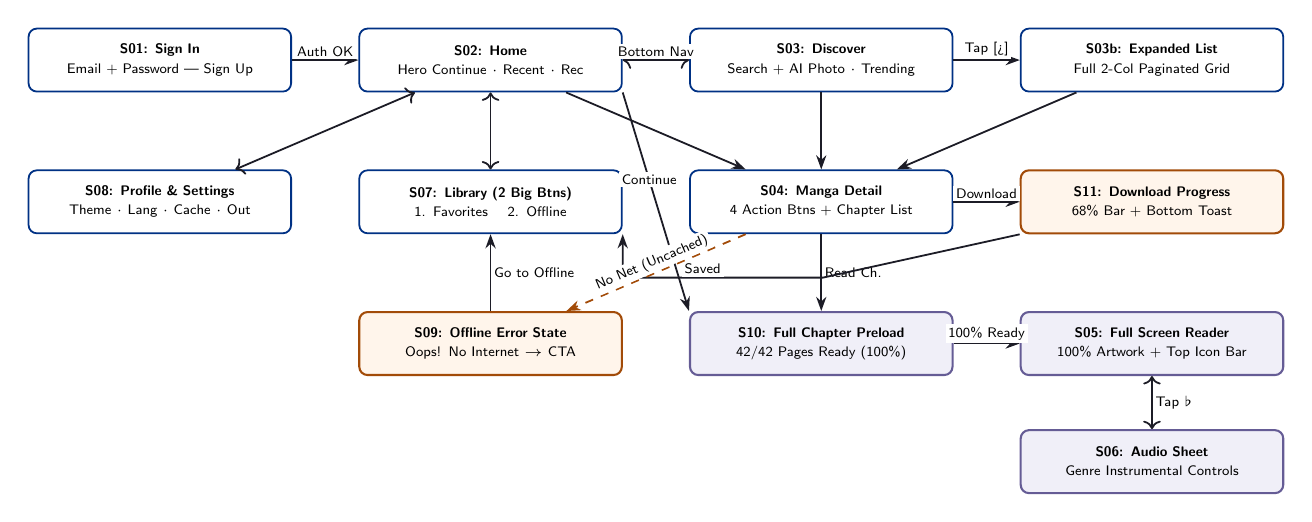
\begin{tikzpicture}[
    scr/.style={draw=hcmutblue!80!black, rounded corners=3pt, fill=white, line width=0.65pt, minimum height=0.8cm, text width=3.1cm, align=center, font=\tiny\sffamily},
    darkscr/.style={draw=naomiaccent!90!black, rounded corners=3pt, fill=naomitint, line width=0.75pt, minimum height=0.8cm, text width=3.1cm, align=center, font=\tiny\sffamily},
    errscr/.style={draw=couldamber!90!black, rounded corners=3pt, fill=orange!8, line width=0.75pt, minimum height=0.8cm, text width=3.1cm, align=center, font=\tiny\sffamily},
    arr/.style={-{Stealth[length=1.8mm,width=1.3mm]}, line width=0.65pt, draw=naomidark},
    darr/.style={-{Stealth[length=1.8mm,width=1.3mm]}, line width=0.65pt, dashed, draw=couldamber!90!black},
    lbl/.style={font=\tiny\sffamily, inner sep=1pt, fill=white}
]
    \node[scr] (s01) at (0,0) {\textbf{S01: Sign In}\\Email + Password | Sign Up};
    \node[scr] (s02) at (4.2,0) {\textbf{S02: Home}\\Hero Continue $\cdot$ Recent $\cdot$ Rec};
    \node[scr] (s03) at (8.4,0) {\textbf{S03: Discover}\\Search + AI Photo $\cdot$ Trending};
    \node[scr] (s03b) at (12.6,0) {\textbf{S03b: Expanded List}\\Full 2-Col Paginated Grid};

    \node[scr] (s08) at (0,-1.8) {\textbf{S08: Profile \& Settings}\\Theme $\cdot$ Lang $\cdot$ Cache $\cdot$ Out};
    \node[scr] (s07) at (4.2,-1.8) {\textbf{S07: Library (2 Big Btns)}\\1. Favorites \quad 2. Offline};
    \node[scr] (s04) at (8.4,-1.8) {\textbf{S04: Manga Detail}\\4 Action Btns + Chapter List};
    \node[errscr] (s11) at (12.6,-1.8) {\textbf{S11: Download Progress}\\68\% Bar + Bottom Toast};

    \node[errscr] (s09) at (4.2,-3.6) {\textbf{S09: Offline Error State}\\Oops! No Internet $\to$ CTA};
    \node[darkscr] (s10) at (8.4,-3.6) {\textbf{S10: Full Chapter Preload}\\42/42 Pages Ready (100\%)};
    \node[darkscr] (s05) at (12.6,-3.6) {\textbf{S05: Full Screen Reader}\\100\% Artwork + Top Icon Bar};
    \node[darkscr] (s06) at (12.6,-5.1) {\textbf{S06: Audio Sheet}\\Genre Instrumental Controls};

    \draw[arr] (s01) -- node[above, lbl]{Auth OK} (s02);
    \draw[arr, <->] (s02) -- node[above, lbl]{Bottom Nav} (s03);
    \draw[arr] (s03) -- node[above, lbl]{Tap [>]} (s03b);
    \draw[arr] (s03b) -- (s04);
    \draw[arr] (s03) -- (s04);
    \draw[arr] (s02) -- (s04);
    \draw[arr, <->] (s02) -- (s07);
    \draw[arr, <->] (s02) -- (s08);
    \draw[arr] (s02.south east) -- node[pos=0.4, lbl]{Continue} (s10.north west);
    \draw[arr] (s04) -- node[right, lbl]{Read Ch.} (s10);
    \draw[arr] (s10) -- node[above, lbl]{100\% Ready} (s05);
    \draw[arr, <->] (s05) -- node[right, lbl]{Tap $\flat$} (s06);
    \draw[arr] (s04) -- node[above, lbl]{Download} (s11);
    \draw[arr] (s11.south west) -- ++(-2.5,-0.55) -| node[pos=0.3, above, lbl]{Saved} (s07.south east);
    \draw[darr] (s04) -- node[above, sloped, lbl]{No Net (Uncached)} (s09);
    \draw[arr] (s09) -- node[right, lbl]{Go to Offline} (s07);
\end{tikzpicture}
\caption{Complete User Flow and Screen Navigation Graph across all 12 frames (\texttt{S01} to \texttt{S11}).}
\label{fig:screen_flow}
\end{figure}

\subsection{High-Fidelity Mobile Mockups \& Screen-by-Screen Specifications}
\label{subsec:hi_fi_mockups}

Figures~\ref{fig:mockups_group1}, \ref{fig:mockups_group2}, and \ref{fig:mockups_group3} present the 12 high-fidelity $390 \times 844\text{ px}$ mobile mockups rendered directly from the \textbf{Naomi} design system, followed by Table~\ref{tab:screen_catalog} detailing the functional components and state coverage of every frame.

\begin{figure}[H]
    \centering
    \begin{subfigure}[b]{0.24\textwidth}
        \centering
        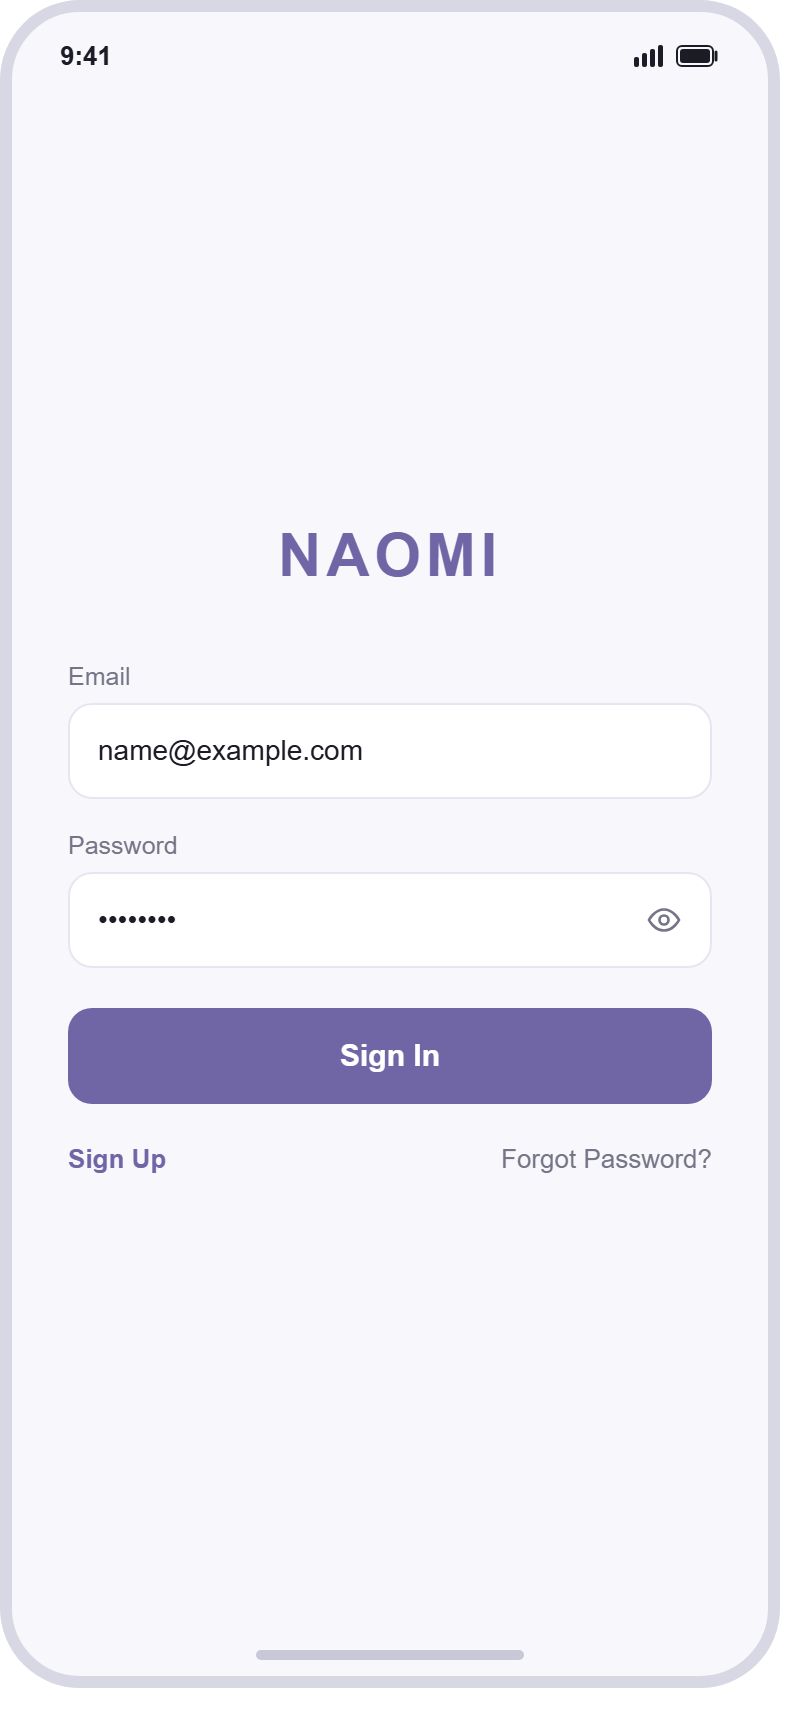
\includegraphics[width=\textwidth]{figures/ui/S01.png}
        \caption{\textbf{S01:} Sign In}
    \end{subfigure}
    \hfill
    \begin{subfigure}[b]{0.24\textwidth}
        \centering
        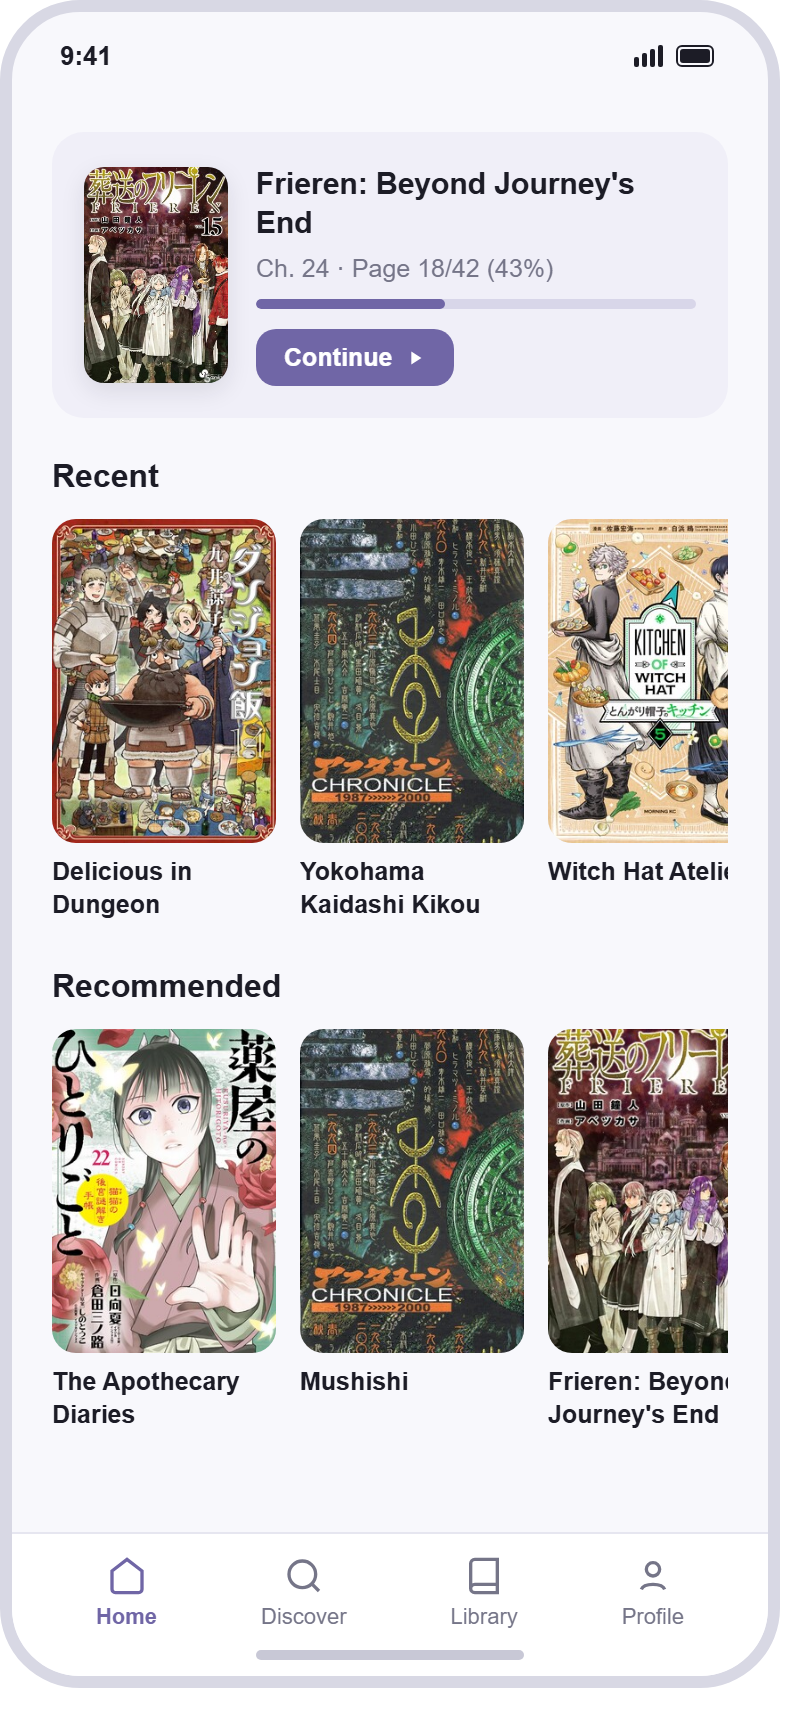
\includegraphics[width=\textwidth]{figures/ui/S02.png}
        \caption{\textbf{S02:} Home Feed}
    \end{subfigure}
    \hfill
    \begin{subfigure}[b]{0.24\textwidth}
        \centering
        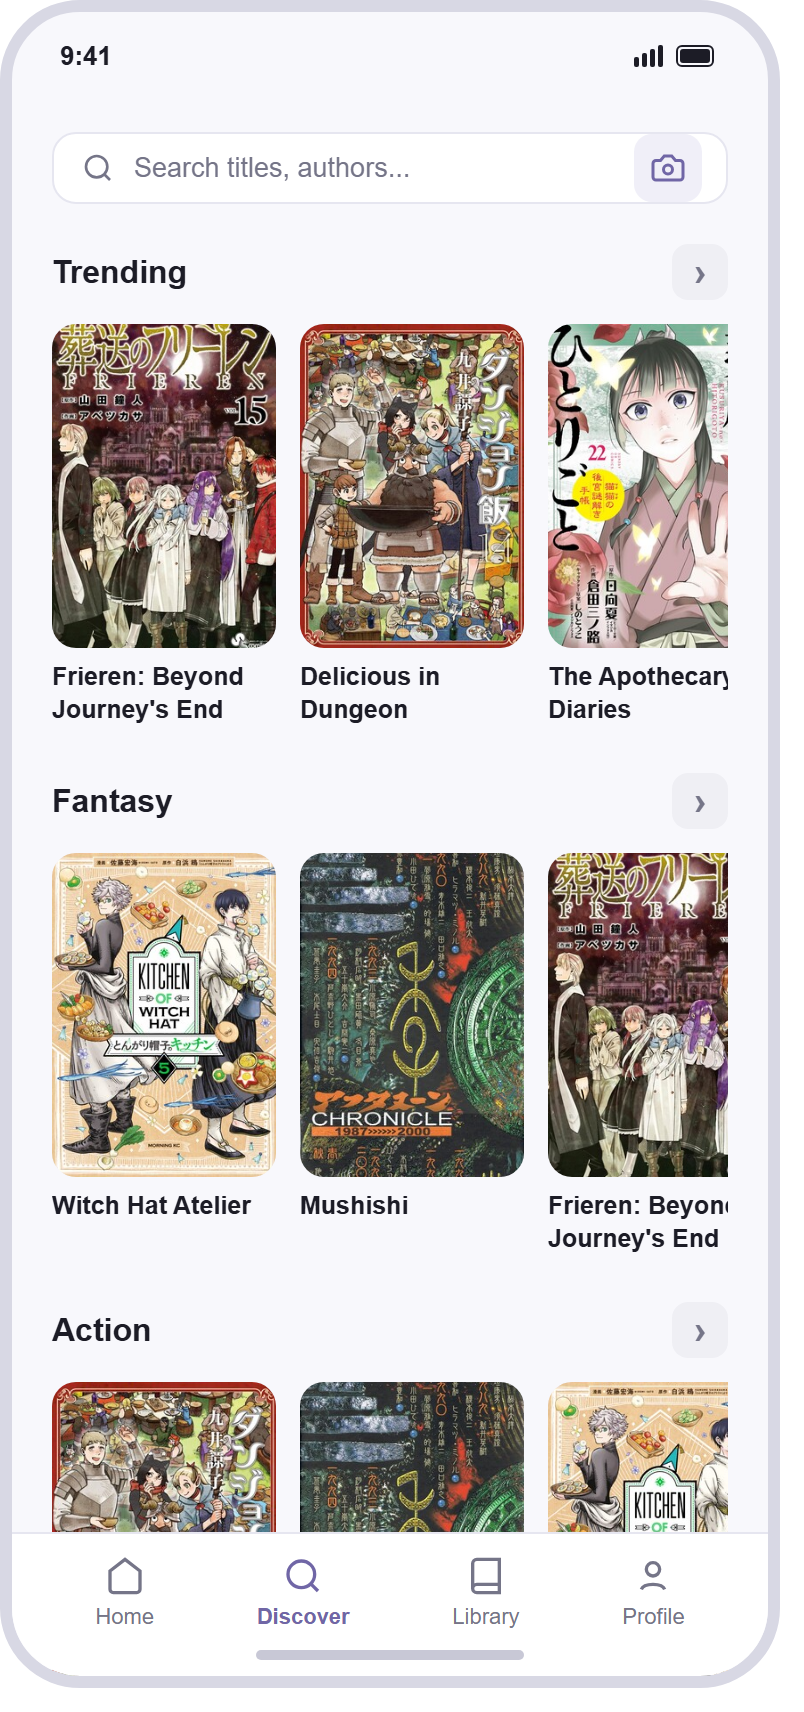
\includegraphics[width=\textwidth]{figures/ui/S03.png}
        \caption{\textbf{S03:} Discover}
    \end{subfigure}
    \hfill
    \begin{subfigure}[b]{0.24\textwidth}
        \centering
        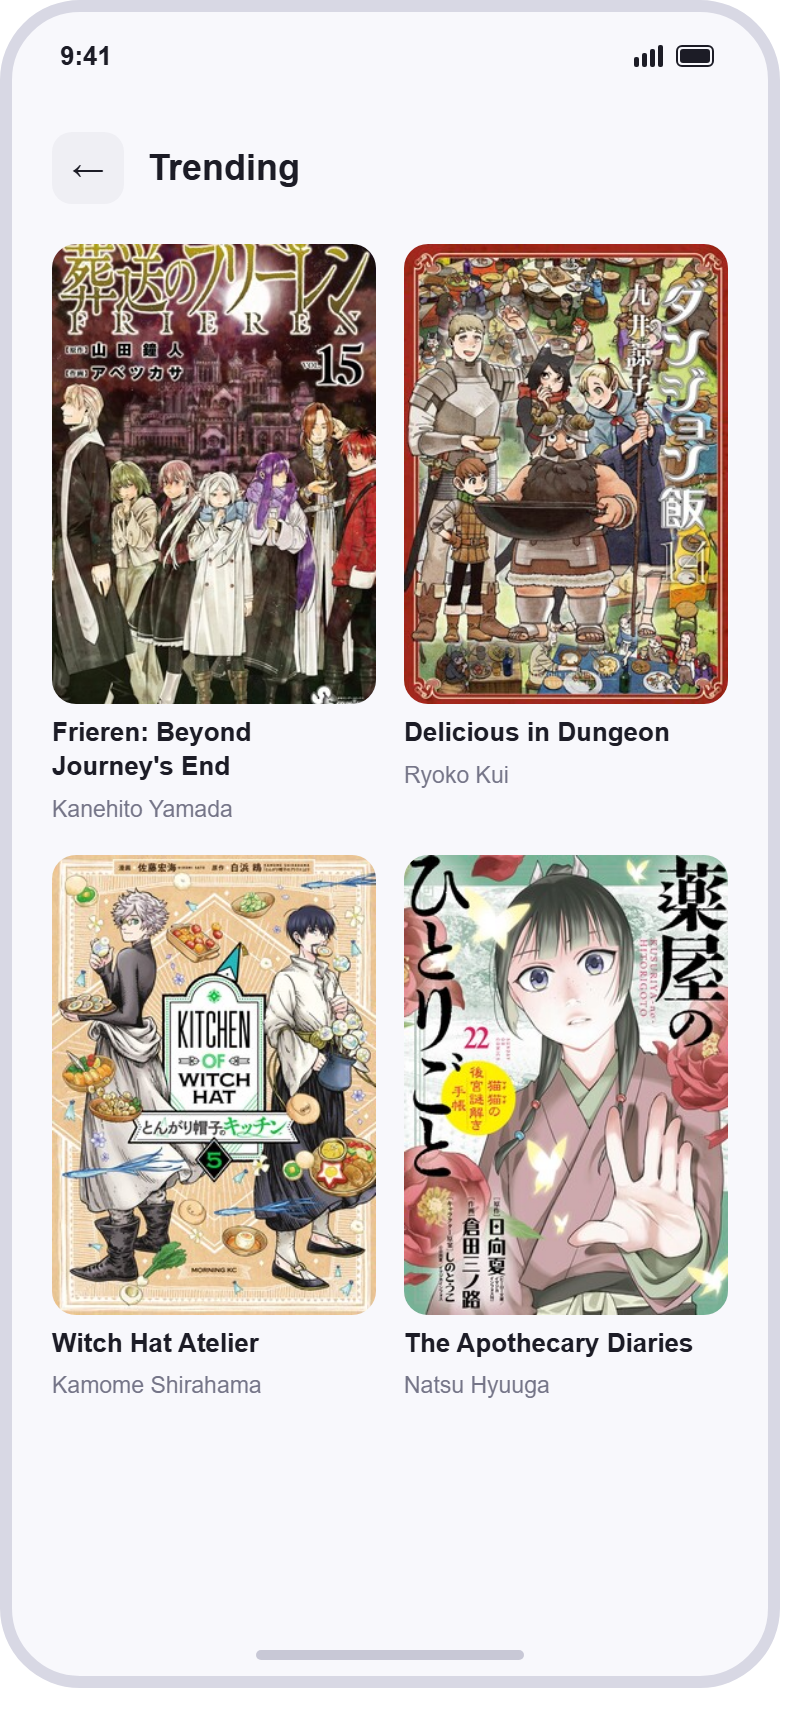
\includegraphics[width=\textwidth]{figures/ui/S03b.png}
        \caption{\textbf{S03b:} Expanded Grid}
    \end{subfigure}
    \caption{High-Fidelity Mockups (Part 1/3): Authentication (\texttt{S01}), 3-Block Home Feed (\texttt{S02}), Discover with AI Photo Search (\texttt{S03}), and Expanded Category Grid (\texttt{S03b}).}
    \label{fig:mockups_group1}
\end{figure}

\begin{figure}[H]
    \centering
    \begin{subfigure}[b]{0.24\textwidth}
        \centering
        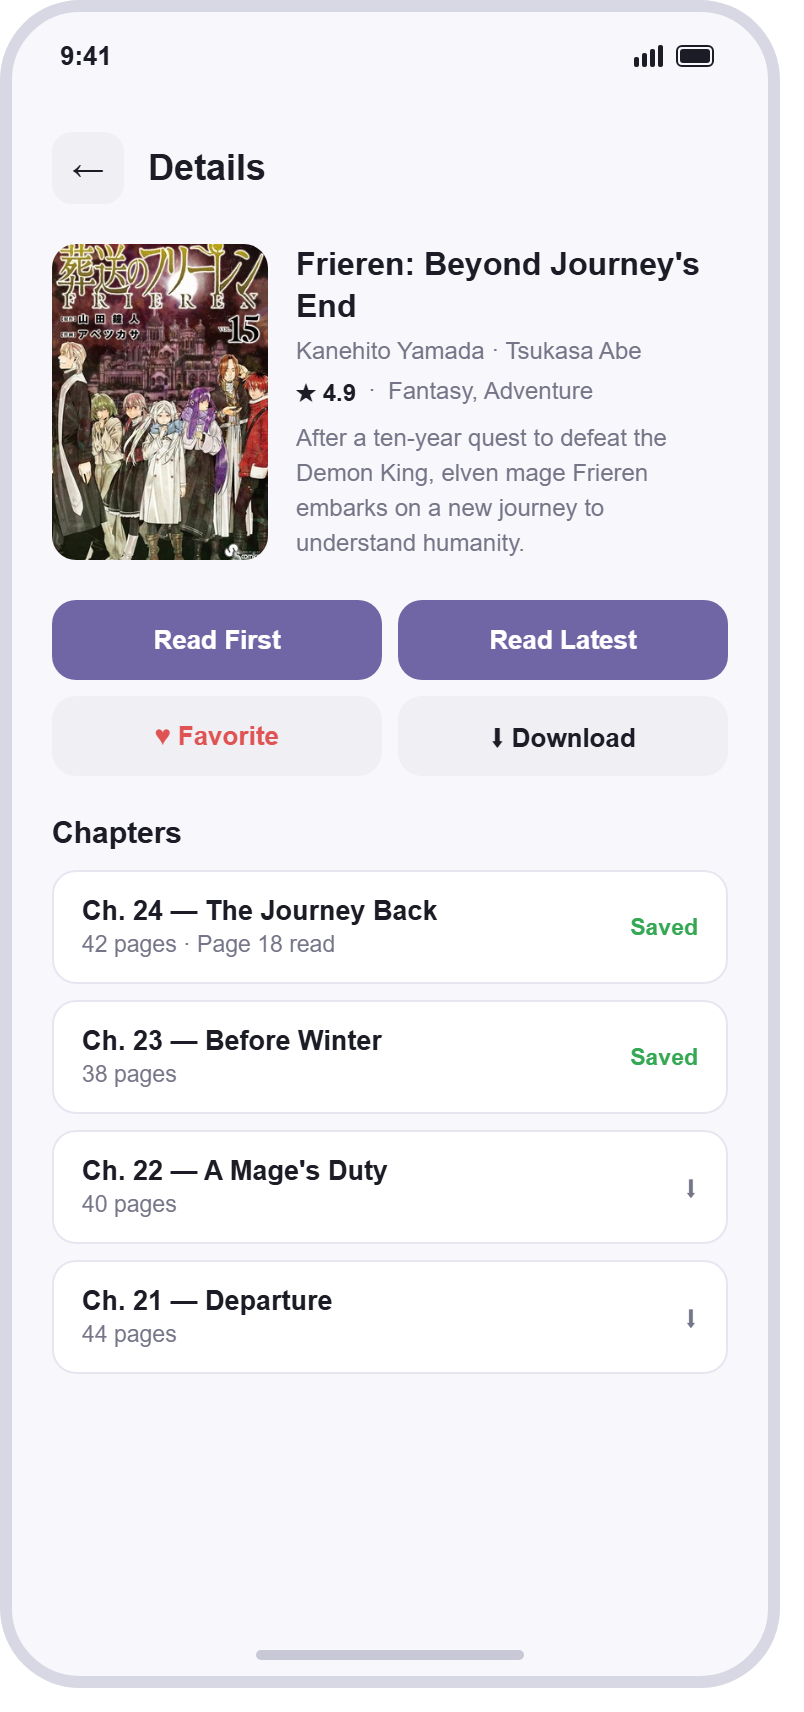
\includegraphics[width=\textwidth]{figures/ui/S04.png}
        \caption{\textbf{S04:} Manga Detail}
    \end{subfigure}
    \hfill
    \begin{subfigure}[b]{0.24\textwidth}
        \centering
        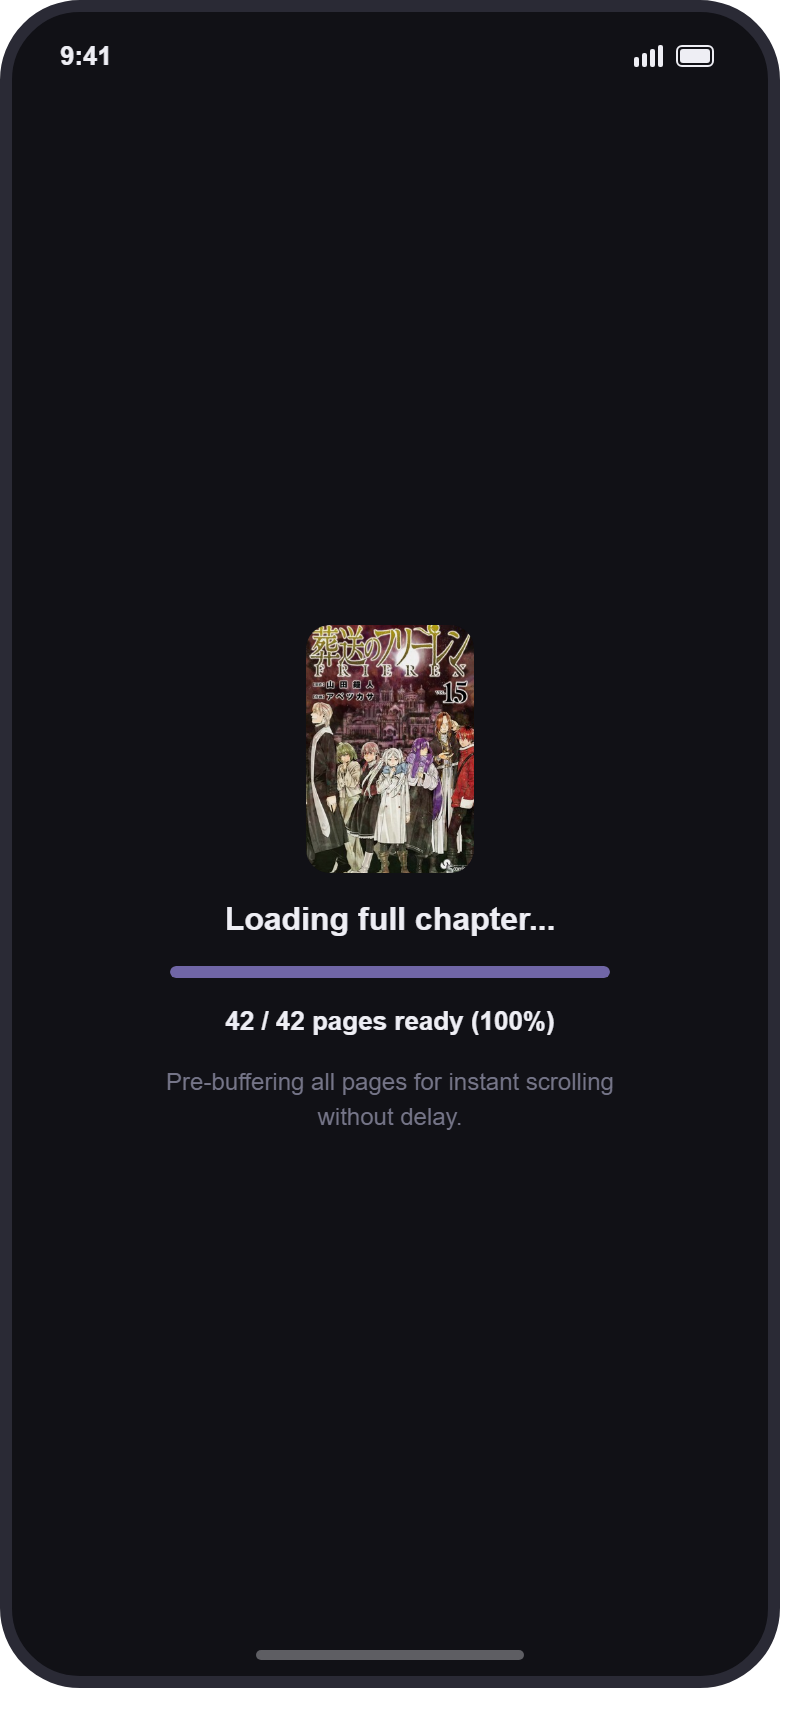
\includegraphics[width=\textwidth]{figures/ui/S10.png}
        \caption{\textbf{S10:} Chapter Preload}
    \end{subfigure}
    \hfill
    \begin{subfigure}[b]{0.24\textwidth}
        \centering
        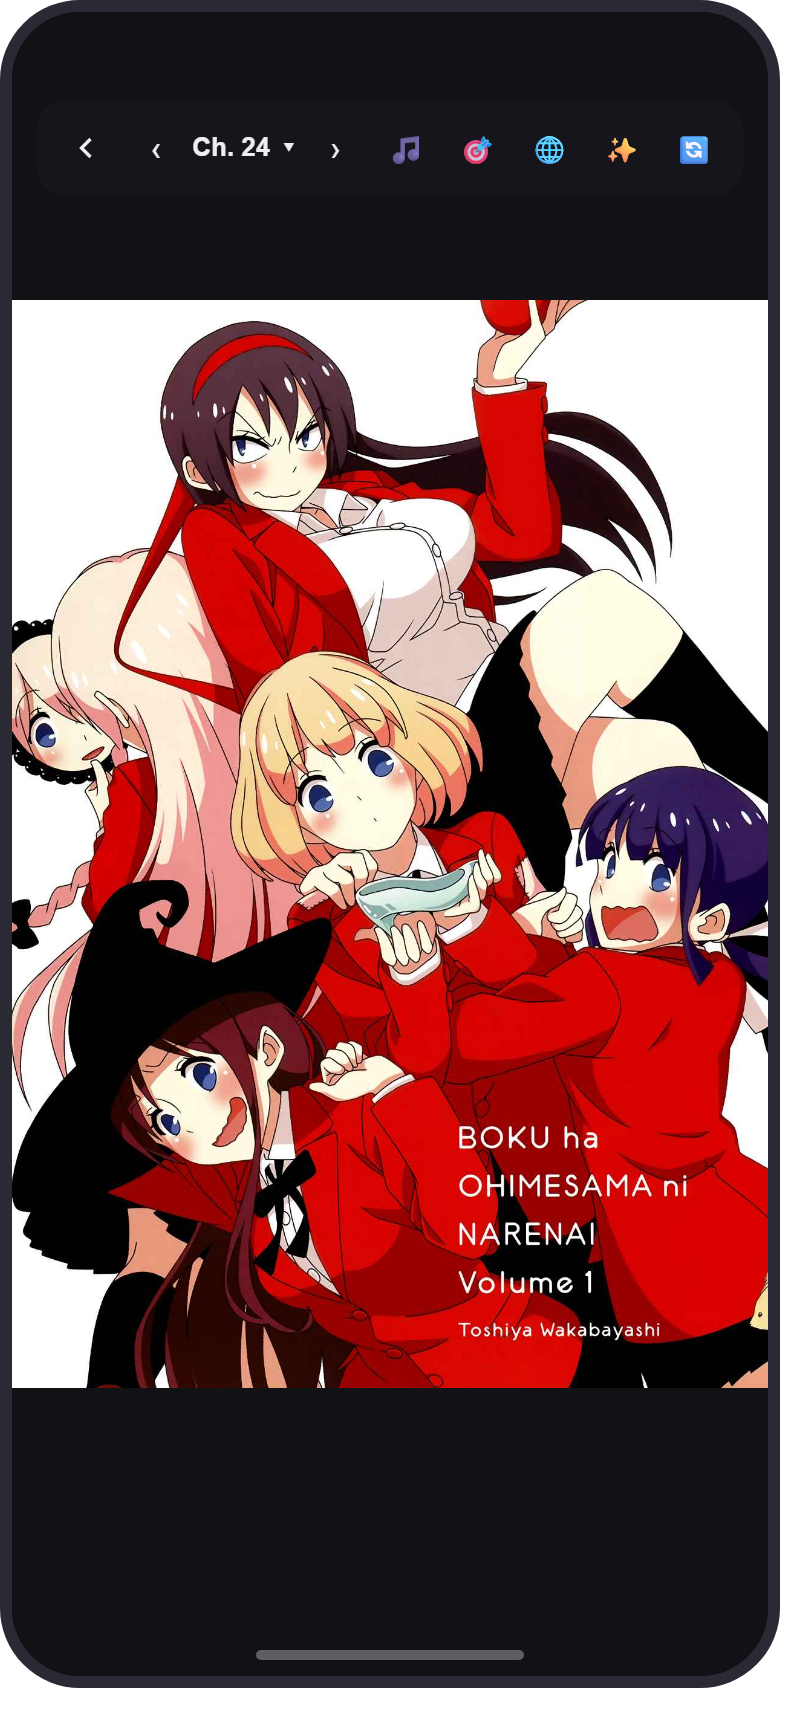
\includegraphics[width=\textwidth]{figures/ui/S05.png}
        \caption{\textbf{S05:} Full Reader}
    \end{subfigure}
    \hfill
    \begin{subfigure}[b]{0.24\textwidth}
        \centering
        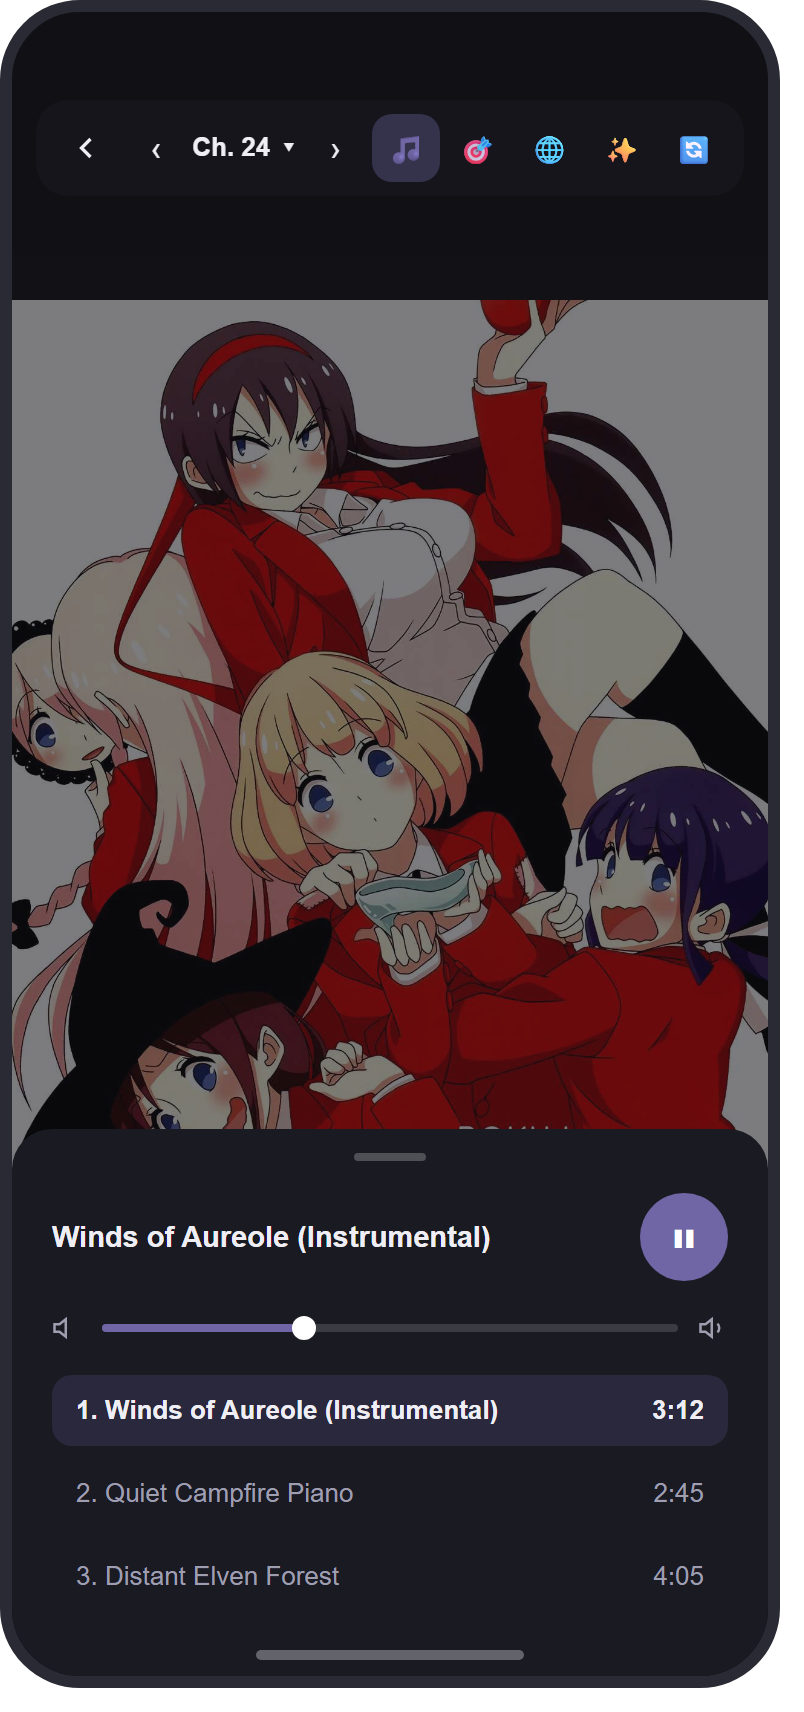
\includegraphics[width=\textwidth]{figures/ui/S06.png}
        \caption{\textbf{S06:} Audio Sheet}
    \end{subfigure}
    \caption{High-Fidelity Mockups (Part 2/3): Manga Detail (\texttt{S04}), Full-Chapter Preload State (\texttt{S10}), 100\% Full-Screen Reader (\texttt{S05}), and Genre Instrumental Audio Sheet (\texttt{S06}).}
    \label{fig:mockups_group2}
\end{figure}

\begin{figure}[H]
    \centering
    \begin{subfigure}[b]{0.24\textwidth}
        \centering
        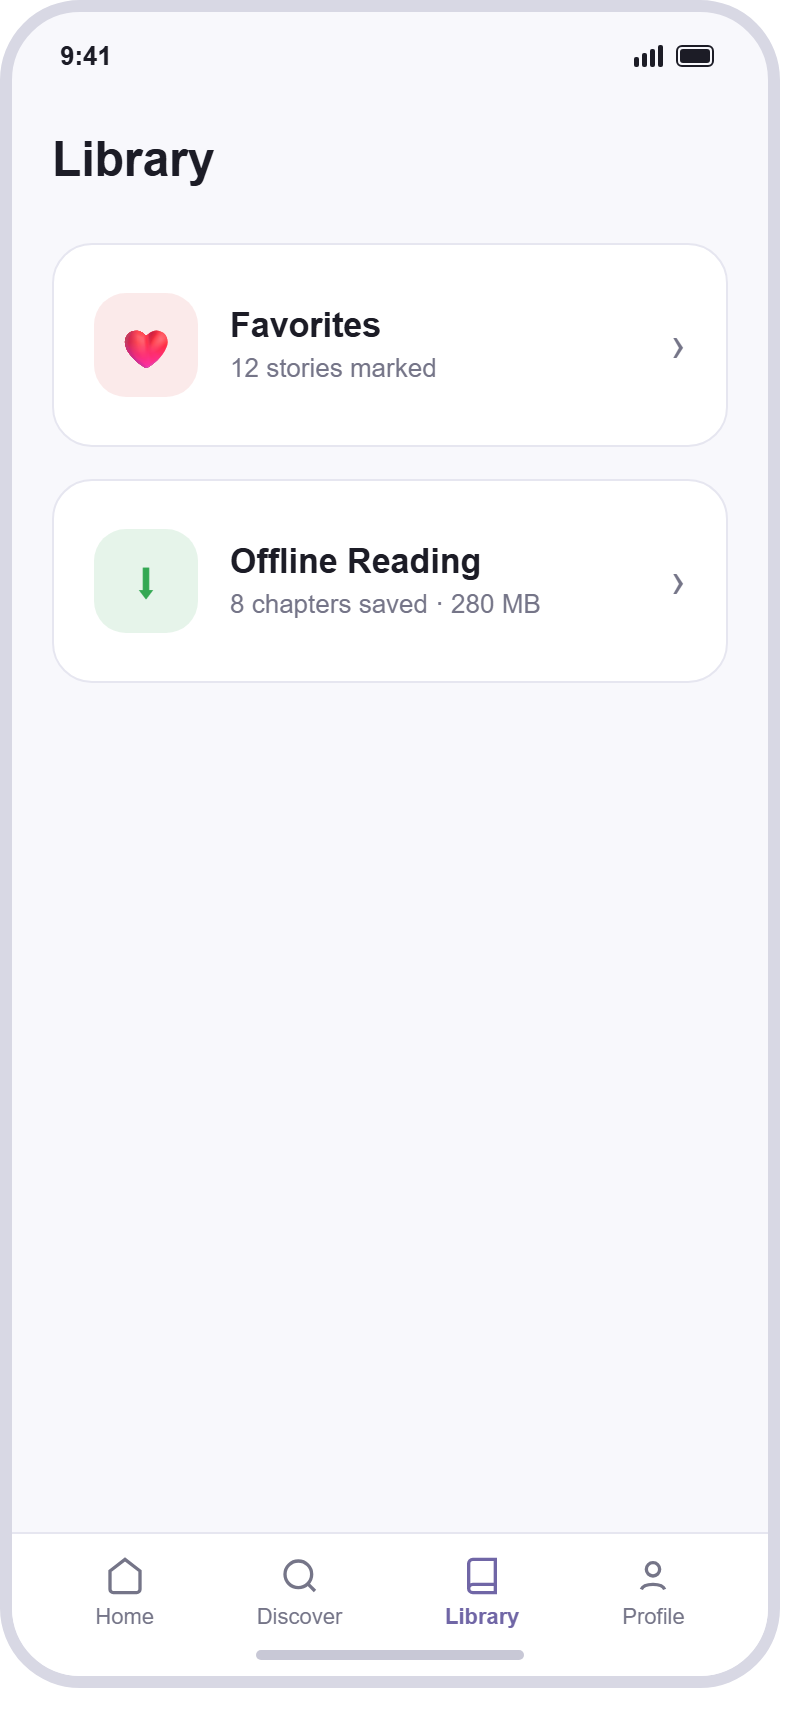
\includegraphics[width=\textwidth]{figures/ui/S07.png}
        \caption{\textbf{S07:} Library Hub}
    \end{subfigure}
    \hfill
    \begin{subfigure}[b]{0.24\textwidth}
        \centering
        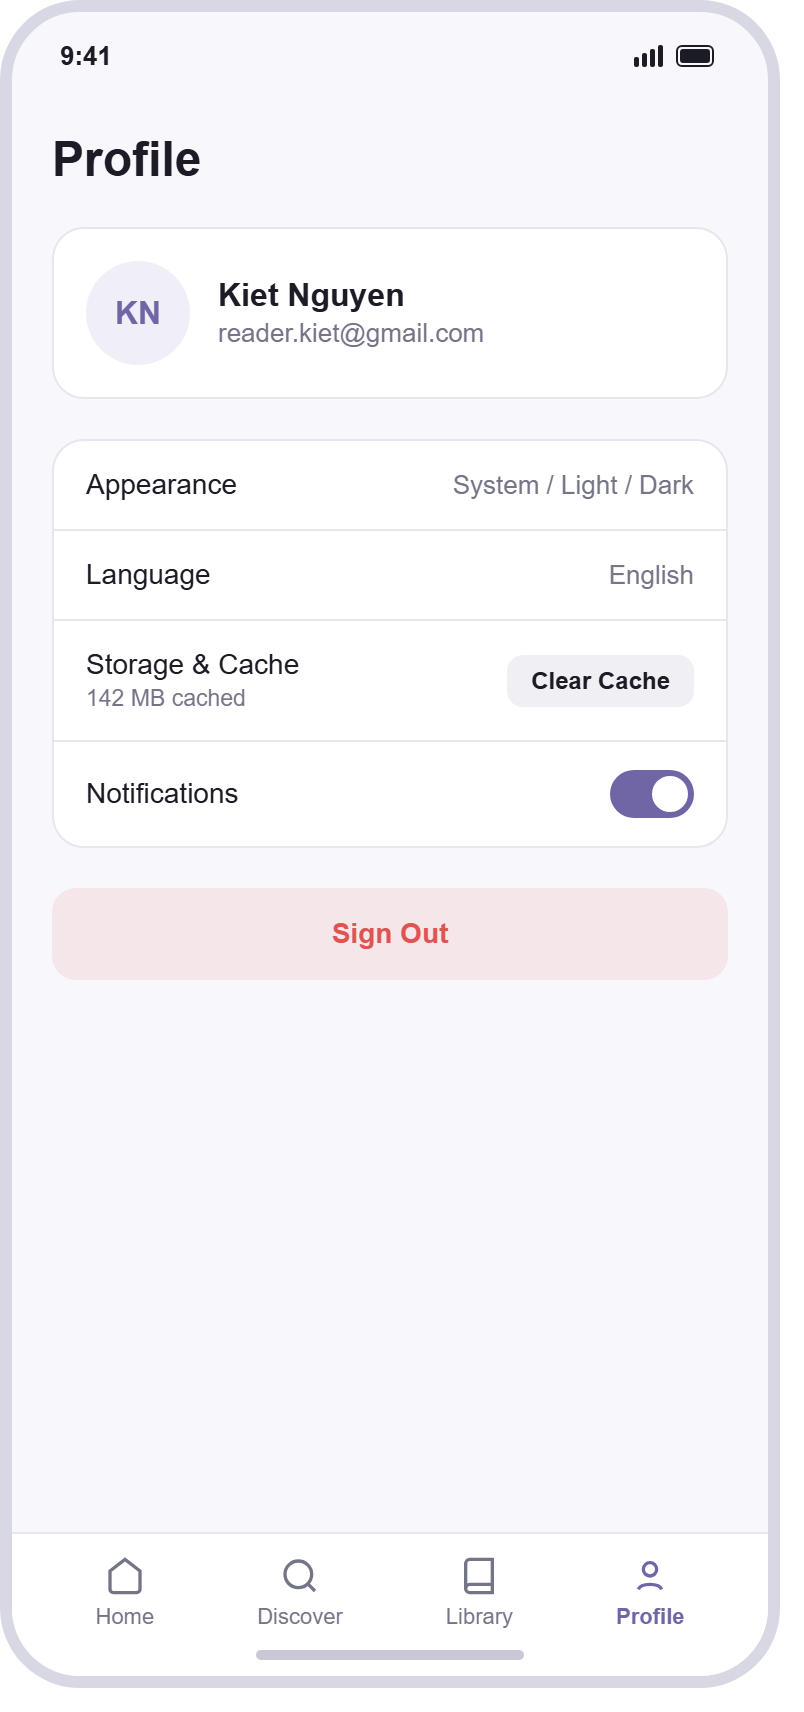
\includegraphics[width=\textwidth]{figures/ui/S08.png}
        \caption{\textbf{S08:} Profile \& Settings}
    \end{subfigure}
    \hfill
    \begin{subfigure}[b]{0.24\textwidth}
        \centering
        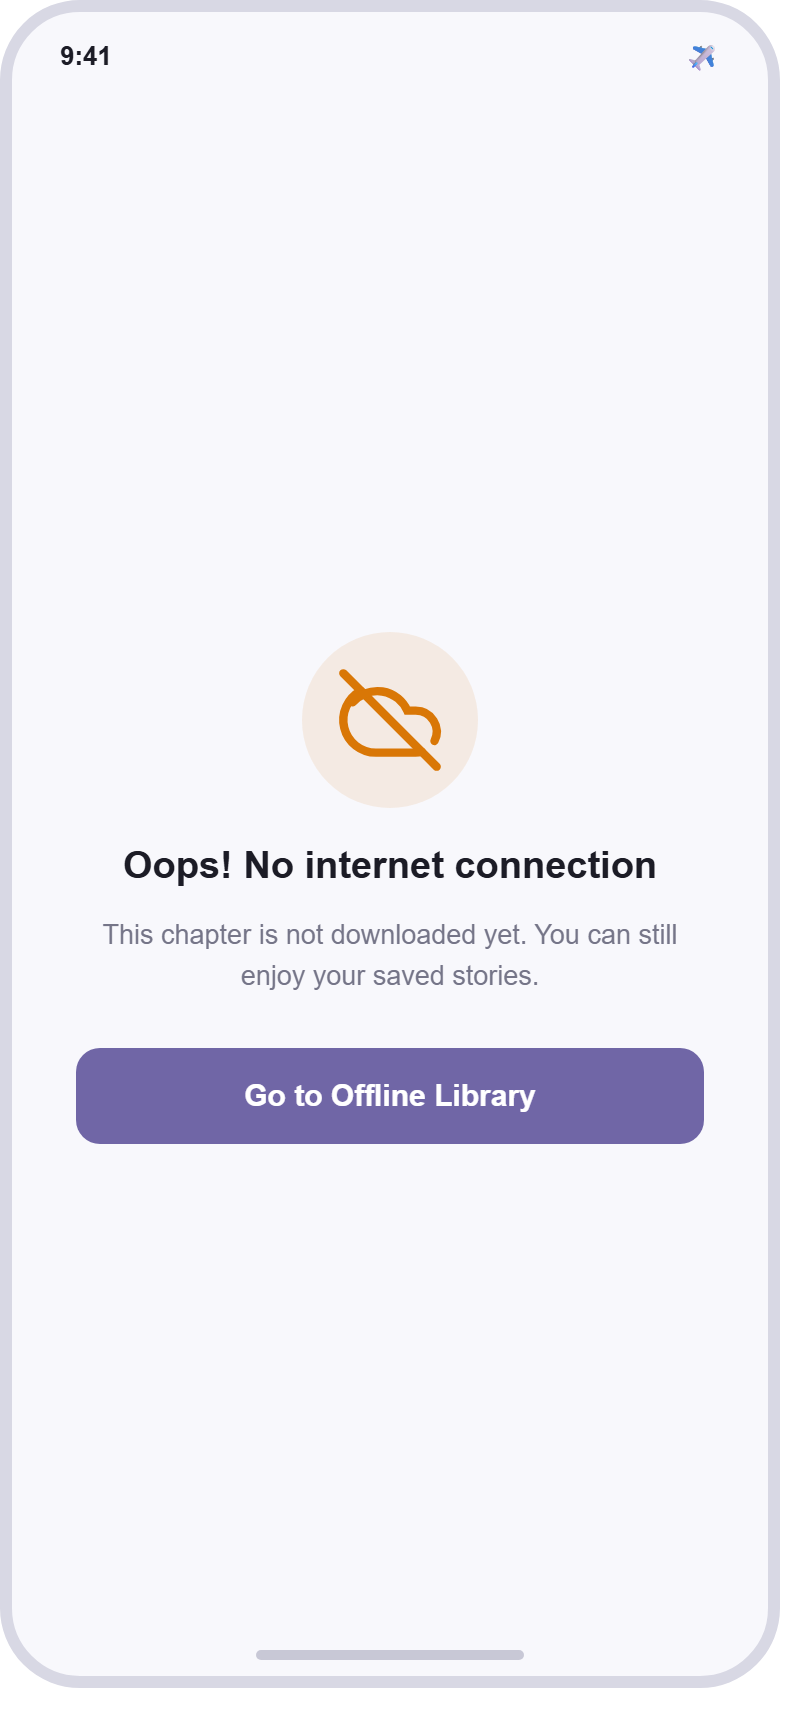
\includegraphics[width=\textwidth]{figures/ui/S09.png}
        \caption{\textbf{S09:} Offline Error}
    \end{subfigure}
    \hfill
    \begin{subfigure}[b]{0.24\textwidth}
        \centering
        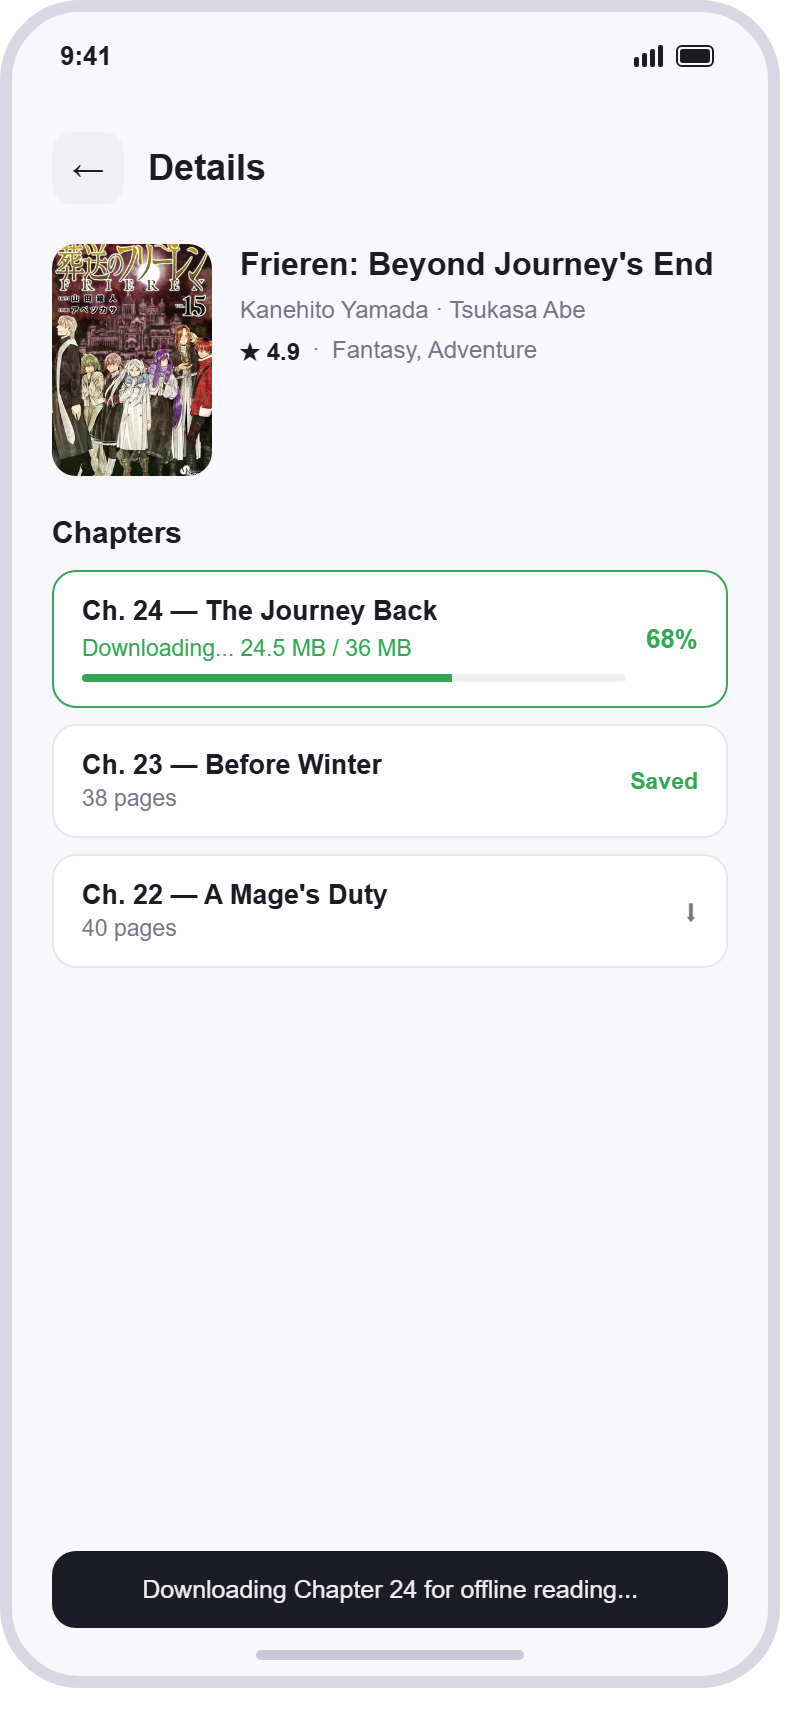
\includegraphics[width=\textwidth]{figures/ui/S11.png}
        \caption{\textbf{S11:} Download (68\%)}
    \end{subfigure}
    \caption{High-Fidelity Mockups (Part 3/3): Two-Button Library (\texttt{S07}), Profile \& Settings (\texttt{S08}), Offline Network Error State (\texttt{S09}), and Real-Time Download Progress State (\texttt{S11}).}
    \label{fig:mockups_group3}
\end{figure}

\begin{table}[H]
\centering
\caption{Comprehensive Specification of all 12 UI/UX Frames (\texttt{S01} to \texttt{S11}) including Primary, Loading, Error, and Offline States.}
\label{tab:screen_catalog}
\scriptsize
\renewcommand{\arraystretch}{1.24}
\begin{tabularx}{\textwidth}{C{1.1cm} L{2.8cm} C{2.1cm} Y}
\toprule
\rowcolor{tablehead}
\textbf{Frame} & \textbf{Screen Title} & \textbf{UI State Role} & \textbf{Key Components, Interactions \& Design Rules} \\
\midrule
\textbf{S01} & \textbf{Sign In} & Auth Entry & Bold lavender \textbf{NAOMI} wordmark (\texttt{\#7066A6}), Email \& Password inputs (\texttt{12px} radius), primary \textbf{Sign In} button, \textbf{Sign Up} and \textbf{Forgot Password?} links. Zero third-party social clutter. \\
\rowcolor{tablerow}
\textbf{S02} & \textbf{Home} & Primary Feed & Strictly 3 blocks: (1) Lavender-tinted \textbf{Continue Reading} Hero card (\textit{Frieren Ch.\ 24 $\cdot$ Page 18/42 (43\%)}) with 1-tap \textbf{Continue $\blacktriangleright$} pill; (2) \textbf{Recent} horizontal scroll; (3) \textbf{Recommended} horizontal scroll + 4-tab Bottom Nav. \\
\textbf{S03} & \textbf{Discover} & Search \& Browse & Search input (\textit{``Search titles, authors...''}) with trailing \textbf{Camera Icon} (invokes zero-permission OS Photo Picker for \texttt{FR-11}), followed by \textbf{Trending} and \textbf{Genre} (\textit{Fantasy, Action}) horizontal rows with \texttt{[>]} expand buttons. \\
\rowcolor{tablerow}
\textbf{S03b} & \textbf{Expanded List} & Category Grid & Full-screen 2-column vertical grid triggered by tapping \texttt{[>]} on \texttt{S03}; includes Back button (\texttt{$\leftarrow$}) and category header. \\
\textbf{S04} & \textbf{Manga Detail} & Series Hub & Cover artwork, title, author (\textit{Kanehito Yamada $\cdot$ Tsukasa Abe}), rating ($\star\ 4.9$), genres, synopsis, 4 action buttons (\textbf{Read First}, \textbf{Read Latest}, \textbf{$\heartsuit$ Favorite}, \textbf{$\downarrow$ Download}), and full chapter list with \textbf{Saved} badges. \\
\rowcolor{tablerow}
\textbf{S10} & \textbf{Full Chapter Preload} & \textbf{Loading State} & AMOLED dark screen (\texttt{\#111116}) with pulsing manga cover, \textit{``Loading full chapter... 42 / 42 pages ready (100\%)''} progress bar, pre-buffering all pages before opening \texttt{S05}. \\
\textbf{S05} & \textbf{Full Screen Reader} & Core Reader & $100\%$ full-screen manga artwork with a single translucent top bar: Back (\texttt{<}), Chapter switcher (\texttt{< Ch.\ 24 $\blacktriangledown$ >}), and 5 pure icons: Music ($\flat$), Focus Mode ($\odot$), Language ($\oplus$), AI Translate ($\star$), and Mode Toggle ($\leftrightarrows$). \\
\rowcolor{tablerow}
\textbf{S06} & \textbf{Audio Sheet} & Modal Overlay & Minimalist bottom sheet over \texttt{S05}: active genre instrumental title (\textit{Winds of Aureole}), $44\text{ px}$ Play/Pause button, smooth volume slider, and 3-row selectable track list for the active genre. \\
\textbf{S07} & \textbf{Library} & Collection Hub & Exactly \textbf{2 Large $20\text{ px}$-Radius Action Buttons}: (1) \textbf{$\heartsuit$ Favorites} (\textit{12 stories marked}) and (2) \textbf{$\downarrow$ Offline Reading} (\textit{8 chapters saved $\cdot$ 280 MB}). \\
\rowcolor{tablerow}
\textbf{S08} & \textbf{Profile \& Settings} & User \& System & Avatar (\texttt{KN}), \textit{Kiet Nguyen (reader.kiet@gmail.com)}, \textbf{Appearance} (\textit{System / Light / Dark}), \textbf{Language} (\textit{English / Tieng Viet}), \textbf{Storage \& Cache} (\textit{142 MB cached} + \textit{Clear Cache}), \textbf{Notifications}, and \textbf{Sign Out}. \\
\textbf{S09} & \textbf{Offline Error State} & \textbf{Error / Empty Fallback} & Triggered within $\le 300\text{ ms}$ when tapping an uncached chapter without Internet: amber offline cloud icon, \textit{``Oops! No internet connection''}, and primary CTA button \textbf{Go to Offline Library} $\to$ \texttt{S07}. \\
\rowcolor{tablerow}
\textbf{S11} & \textbf{Download in Progress} & \textbf{Active Progress State} & Highlights Chapter 24 row in sage green (\texttt{\#34A853}) with live progress bar (\textit{``Downloading... 24.5 MB / 36 MB -- 68\%''}) and bottom toast banner (\textit{``Downloading Chapter 24 for offline reading...''}). \\
\bottomrule
\end{tabularx}
\end{table}

\newpage
\section{Traceability Matrix \& Document Quality Assurance}
\label{sec:traceability}

\subsection{End-to-End Bidirectional Traceability Methodology}
\label{subsec:traceability_method}

In accordance with software engineering best practices (\textit{Sommerville, Software Engineering, 10th Ed., Chapter 4 -- Requirements Management}) and Rubric Criterion 1.7, a production-grade specification must establish \textbf{End-to-End Bidirectional Traceability} across all five engineering layers:
\begin{center}
\footnotesize
\textbf{Elicitation (Sec.\ 1.1)} $\longleftrightarrow$ \textbf{FR/NFR (Sec.\ 1.2, 1.3)} $\longleftrightarrow$ \textbf{UC/US (Sec.\ 1.2)}\\
$\longleftrightarrow$ \textbf{UI Mockups (Sec.\ 1.6)} $\longleftrightarrow$ \textbf{Architecture, DB \& APIs (Sec.\ 1.4, 1.5)}
\end{center}
This rigorous linkage guarantees two vital properties for Assignment 02:
\begin{enumerate}
    \item \textbf{Zero Gold-Plating (Forward Traceability):} Every UI frame (\texttt{S01}--\texttt{S11}), BLoC state controller, relational database table, and REST API endpoint exists solely to fulfil one or more empirically elicited user requirements.
    \item \textbf{100\% Acceptance Coverage (Backward Traceability):} Every \texttt{MUST-HAVE}, \texttt{SHOULD-HAVE}, and \texttt{COULD-HAVE} requirement is backed by concrete architectural components, normalised database tables, API contracts, and testable Gherkin BDD scenarios.
\end{enumerate}

\subsection{Functional Requirements Master Traceability Matrix}
\label{subsec:fr_traceability}

Table~\ref{tab:fr_traceability} maps $100\%$ of the Functional Requirements (\texttt{FR-00} through \texttt{FR-16}) across their elicitation origins, Use Cases/User Stories, UI Mockup Screens, In-App Clean Architecture components, Database Tables, and REST API endpoints.

\begin{scriptsize}
\renewcommand{\arraystretch}{1.22}
\setlength{\tabcolsep}{2.5pt}
\begin{longtable}{C{1.1cm} L{2.4cm} C{1.45cm} L{1.7cm} C{1.2cm} C{1.2cm} L{3.3cm} L{2.75cm}}
\caption{Master Bidirectional Traceability Matrix for Functional Requirements (\texttt{FR-00} to \texttt{FR-16}).}
\label{tab:fr_traceability} \\
\toprule
\rowcolor{tablehead}
\textbf{FR ID} & \textbf{Requirement Summary} & \textbf{MoSCoW} & \textbf{Elicitation} & \textbf{UC / US} & \textbf{UI Screen} & \textbf{Clean Architecture} & \textbf{DB \& APIs} \\
\midrule
\endfirsthead
\multicolumn{8}{c}{{\bfseries \tablename\ \thetable{} -- continued from previous page}} \\
\toprule
\rowcolor{tablehead}
\textbf{FR ID} & \textbf{Requirement Summary} & \textbf{MoSCoW} & \textbf{Elicitation} & \textbf{UC / US} & \textbf{UI Screen} & \textbf{Clean Architecture} & \textbf{DB \& APIs} \\
\midrule
\endhead
\midrule \multicolumn{8}{r}{{Continued on next page}} \\ \bottomrule
\endfoot
\bottomrule
\endlastfoot

\mbox{\textbf{FR-00}} & User Account Auth (Sign Up, Sign In, Reset) & \textbf{MUST} & Pain Point \#7 (Cloud sync) & \texttt{UC-00}\newline \texttt{US-00} & \textbf{S01}, \textbf{S08} & \texttt{AuthBloc} $\to$ \allowbreak\texttt{SignInUseCase} $\to$ \allowbreak\texttt{AuthRepoImpl} $\to$ \allowbreak\texttt{SecureStorage} & Table \texttt{users}\newline \textbf{API 04} (\texttt{/auth/v1/token}) \\
\rowcolor{tablerow}
\mbox{\textbf{FR-01}} & Discover \& Search (Trending, Genres, Expand) & \textbf{MUST} & Pain Point \#3, Q2 ($75\%$ catalog) & \texttt{UC-01}\newline \texttt{US-01} & \textbf{S03}, \textbf{S03b} & \texttt{DiscoverBloc} $\to$ \allowbreak\texttt{SearchComicsUseCase} $\to$ \allowbreak\texttt{ComicRepoImpl} & \texttt{comics, genres, comic\_\allowbreak genres}\newline \textbf{API 01} (\texttt{GET /manga}) \\
\mbox{\textbf{FR-02}} & Full-Screen Reader \& Focus Mode & \textbf{MUST} & Persona 1, Q2 ($100\%$ hate ad clutter) & \texttt{UC-03, UC-05}\newline \texttt{US-03, US-05} & \textbf{S10}, \textbf{S05} & \texttt{ReaderBloc} $\to$ \allowbreak\texttt{Get\allowbreak Chapter\allowbreak Content\allowbreak UseCase} $\to$ \allowbreak\texttt{ComicRepoImpl} & \texttt{chapters, pages}\newline \textbf{API 03} (\texttt{/at-home/server}) \\
\rowcolor{tablerow}
\mbox{\textbf{FR-03}} & Dual Reader Mode Toggle (Webtoon $\leftrightarrow$ Manga) & \textbf{MUST} & Persona 1, Q5 ($25\%$ mode toggle) & \texttt{UC-03}\newline \texttt{US-03} & \textbf{S05} (Icon $\leftrightarrows$) & \texttt{ReaderBloc} (\texttt{ToggleModeEvent}) $\to$ \allowbreak\texttt{ComicRepoImpl} & \texttt{pages}, \texttt{users.preferences}\newline Local Drift SQLite \\
\mbox{\textbf{FR-04}} & Auto-Save Page Progress \& Instant Resume & \textbf{MUST} & Persona 3, Q5 ($75\%$ page history) & \texttt{UC-05}\newline \texttt{US-05} & \textbf{S02} (Hero), \textbf{S05} & \texttt{ReaderBloc} $\to$ \allowbreak\texttt{Save\allowbreak Reading\allowbreak Progress\allowbreak UseCase} $\to$ \allowbreak\texttt{DriftDB} & \texttt{reading\_\allowbreak history}\newline \textbf{API 05} (\texttt{/reading\_history}) \\
\rowcolor{tablerow}
\mbox{\textbf{FR-05}} & Genre-Matched Instrumental Ambient Audio & \textbf{MUST} & Persona 1, Q3 ($100\%$), Q4 ($3.75/5$) & \texttt{UC-04}\newline \texttt{US-04} & \textbf{S05}~(Icon~\musicnote), \textbf{S06} & \texttt{AudioCubit} $\to$ \allowbreak\texttt{Get\allowbreak Genre\allowbreak Audio\allowbreak UseCase} $\to$ \allowbreak\texttt{JustAudioService} & \texttt{ambient\_\allowbreak tracks, genres}\newline \textbf{API 07} (\texttt{/ambient\_tracks}) \\
\mbox{\textbf{FR-06}} & Offline Chapter Download with Live Progress & \textbf{MUST} & Persona 2, Q2 ($50\%$ offline/VIP) & \texttt{UC-06}\newline \texttt{US-06} & \textbf{S04}, \textbf{S11} & \texttt{DownloadBloc} $\to$ \allowbreak\texttt{Download\allowbreak Mgr\allowbreak Service} $\to$ \allowbreak\texttt{LocalFileStorage} & \texttt{offline\_\allowbreak downloads}\newline \textbf{API 03} (\texttt{/at-home/server}) \\
\rowcolor{tablerow}
\mbox{\textbf{FR-07}} & Personal Library (Favorites \& Offline Reading) & \textbf{MUST} & Persona 2, Q5 (Library categories) & \texttt{UC-07}\newline \texttt{US-07} & \textbf{S07} (2 Big Btns) & \texttt{LibraryBloc} $\to$ \allowbreak\texttt{Get\allowbreak Library\allowbreak UseCase} $\to$ \allowbreak\texttt{ComicRepoImpl} & \texttt{bookmarks, offline\_\allowbreak downloads}\newline \textbf{API 06} (\texttt{/bookmarks}) \\
\textbf{FR-08} & Consolidated Home Feed (Continue, Recent, Rec) & \textbf{SHOULD} & Persona 3, Q5 ($75\%$ genre recs) & \texttt{UC-01, UC-05}\newline \texttt{US-01, US-05} & \textbf{S02} & \texttt{HomeBloc} $\to$ \allowbreak\texttt{Get\allowbreak Home\allowbreak Feed\allowbreak UseCase} $\to$ \allowbreak\texttt{ComicRepoImpl} & \texttt{reading\_\allowbreak history, comics, genres}\newline \textbf{API 01 \& API 05} \\
\rowcolor{tablerow}
\mbox{\textbf{FR-09}} & Minimalist Audio Sheet Controls \& Focus Pause & \textbf{SHOULD} & Persona 1, Q4 (Ambient controls) & \texttt{UC-04}\newline \texttt{US-04} & \textbf{S06} & \texttt{AudioCubit} $\to$ \allowbreak\texttt{JustAudioService} (\texttt{AudioSession}) & \texttt{ambient\_\allowbreak tracks}\newline \textbf{API 07} (\texttt{/ambient\_tracks}) \\
\mbox{\textbf{FR-10}} & Comic Detail View \& 4 Quick Chapter Actions & \textbf{SHOULD} & Persona 2, Persona 3 & \texttt{UC-02}\newline \texttt{US-02} & \textbf{S04} & \texttt{ComicDetailBloc} $\to$ \allowbreak\texttt{Get\allowbreak Comic\allowbreak Detail\allowbreak UseCase} $\to$ \allowbreak\texttt{ComicRepoImpl} & \texttt{comics, chapters, bookmarks}\newline \textbf{API 02 \& API 06} \\
\rowcolor{tablerow}
\mbox{\textbf{FR-11}} & Zero-Permission Visual Search (Photo Picker) & \textbf{COULD} & Persona 2, Q5 ($50\%$ visual search) & \texttt{UC-01}\newline \texttt{US-01} & \textbf{S03} (Camera) & \texttt{DiscoverBloc} $\to$ \allowbreak\texttt{Visual\allowbreak Search\allowbreak UseCase} $\to$ \allowbreak\texttt{SystemPhotoPicker} & \texttt{comics}\newline \textbf{API 01} (\texttt{GET /manga}) \\
\mbox{\textbf{FR-12}} & In-Place AI Chapter Translation & \textbf{COULD} & Persona 3, Q5 ($100\%$ AI translate) & \texttt{UC-03}\newline \texttt{US-03} & \textbf{S05} (Icon $\star$) & \texttt{ReaderBloc} (\texttt{TranslateEvent}) $\to$ \allowbreak\texttt{Ai\allowbreak Translation\allowbreak Service} & \texttt{pages} (In-memory translated overlay cache) \\
\rowcolor{tablerow}
\mbox{\textbf{FR-13}} & Offline Network Loss Error State \& Routing & \textbf{SHOULD} & Persona 2, Q2 ($50\%$ network drop) & \texttt{UC-06}\newline \texttt{US-06} & \textbf{S09} $\to$ \textbf{S07} & \texttt{ConnectivityCubit} (\texttt{ConnectivityPlus}) $\to$ \allowbreak\texttt{ReaderBloc} & \texttt{offline\_\allowbreak downloads} (Local SQLite Drift) \\
\mbox{\textbf{FR-14}} & Profile \& System Settings (Theme, Lang, Cache) & \textbf{SHOULD} & Q1 (Day/Night), Pain Point \#4 & \texttt{UC-08}\newline \texttt{US-08} & \textbf{S08} & \texttt{SettingsCubit} $\to$ \allowbreak\texttt{CacheMgrService} \& \texttt{AuthBloc} & \texttt{users.preferences} (JSONB) + Tier 4 LRU Cache \\
\rowcolor{tablerow}
\mbox{\textbf{FR-15}} & In-App Purchases (IAP) / Virtual Coins & \textbf{WON'T} & $100\%$ Free, Non-Commercial Rule & Excluded & None & Excluded (Zero payment/ad SDKs) & None \\
\mbox{\textbf{FR-16}} & Social Feed \& 1-on-1 Direct Messaging & \textbf{WON'T} & Content-First Focus Philosophy & Excluded & None & Excluded & None \\
\end{longtable}
\end{scriptsize}

\subsection{Non-Functional Requirements Traceability Matrix}
\label{subsec:nfr_traceability}

Table~\ref{tab:nfr_traceability} traces all 18 Non-Functional Requirements (\texttt{NFR-01} to \texttt{NFR-18}) to their corresponding UI screens, architectural/database mechanisms, and Assignment 02 QA verification tools.

\begin{table}[H]
\centering
\caption{Bidirectional Traceability Matrix for Non-Functional Requirements (\texttt{NFR-01} to \texttt{NFR-18}).}
\label{tab:nfr_traceability}
\scriptsize
\renewcommand{\arraystretch}{1.12}
\setlength{\tabcolsep}{3.0pt}
\begin{tabularx}{\textwidth}{C{1.35cm} L{3.1cm} C{1.55cm} Y L{2.9cm}}
\toprule
\rowcolor{tablehead}
\textbf{NFR ID} & \textbf{SMART Criterion \& Threshold} & \textbf{UI Screens} & \textbf{Architectural \& Data Engineering Mechanism (Sec.\ 4 \& 5)} & \textbf{Verification Tool} \\
\midrule
\mbox{\textbf{NFR-01}} & Cold Start Time $\le 2.0\text{ s}$ & \textbf{S01, S02} & Lazy service DI; render initial \texttt{S02} frame from local SQLite Drift prior to network sync. & Android Vitals / DevTools \\
\rowcolor{tablerow}
\mbox{\textbf{NFR-02}} & Warm Start Time $\le 0.8\text{ s}$ & All Screens & Retain \texttt{BLoC} state in memory; fast AES-256 session restore via \texttt{FlutterSecureStorage}. & Flutter DevTools \\
\mbox{\textbf{NFR-03}} & Reader Scrolling $\ge 60\text{ FPS}$ ($\le 16.6\text{ ms}$) & \textbf{S05} & Impeller/Skia engine + virtualised viewport list + file-system page storage (no SQLite BLOBs). & Performance Overlay \\
\rowcolor{tablerow}
\mbox{\textbf{NFR-04}} & Chapter Preload Initiation $\le 1.5\text{ s}$ & \textbf{S10} $\to$ \textbf{S05} & Concurrent page pre-buffering from \texttt{MangaDex@Home} CDN (\texttt{API 03}) on \texttt{S10}. & Network Profiler \\
\mbox{\textbf{NFR-05}} & Auth Response Time $\le 1.0\text{ s}$ & \textbf{S01} & Lightweight \texttt{POST /auth/v1/token} (\texttt{API 04}) endpoint over TLS 1.3. & Postman / Profiler \\
\rowcolor{tablerow}
\mbox{\textbf{NFR-06}} & Peak Runtime RAM $\le 250\text{ MB}$ & \textbf{S05, S10} & Recycle off-screen GPU page textures outside the $\pm 2$-page viewport window. & Android Memory Profiler \\
\mbox{\textbf{NFR-07}} & Temporary Disk Cache $\le 500\text{ MB}$ & \textbf{S08} & Tier 4 LRU cache eviction worker auto-pruning to $350\text{ MB}$ + manual \textit{Clear Cache} on \texttt{S08}. & File Storage Inspector \\
\rowcolor{tablerow}
\mbox{\textbf{NFR-08}} & Offline Fallback Latency $\le 300\text{ ms}$ & \textbf{S09} $\to$ \textbf{S07} & Reactive \texttt{ConnectivityPlus} stream listener routing uncached offline requests to \texttt{S09}. & Connectivity Listener \\
\mbox{\textbf{NFR-09}} & Local SQLite I/O $\le 50\text{ ms}$/query & \textbf{S02, S05, S07} & Indexed foreign/unique keys \texttt{(user\_id, chapter\_id)} and asynchronous Drift isolates. & SQLite Benchmark \\
\rowcolor{tablerow}
\mbox{\textbf{NFR-10}} & Hardware Token Encryption \textbf{AES-256} & \textbf{S01, S08} & Tier 1 \texttt{FlutterSecureStorage} backed by Android Keystore and iOS Keychain. & Security / Root Audit \\
\mbox{\textbf{NFR-11}} & Transport Security \textbf{100\% TLS 1.3} & \textbf{API 01--07} & \texttt{usesCleartextTraffic="false"} in \texttt{AndroidManifest.xml} + Supabase PostgreSQL RLS. & Charles Proxy / Audit \\
\rowcolor{tablerow}
\mbox{\textbf{NFR-12}} & \textbf{0 Dangerous OS Permissions} & \textbf{S03} & OS \texttt{System Photo Picker} for Visual Search (\texttt{FR-11}); zero Camera/Storage/GPS permissions. & \texttt{Android\allowbreak Manifest.xml} \\
\mbox{\textbf{NFR-13}} & Graceful Permission Denial Handling & \textbf{S08, S11} & Non-crashing runtime handling of \texttt{POST\_NOTIFICATIONS}; fallback to in-app toast on \texttt{S11}. & Manual UI Test Case \\
\rowcolor{tablerow}
\mbox{\textbf{NFR-14}} & Android 8.0+ (API 26--34) \& iOS 13+ & All Screens & Configured in \texttt{build.gradle} (\texttt{minSdkVersion 26, targetSdkVersion 34}) \& \texttt{Podfile}. & Firebase Test Lab \\
\mbox{\textbf{NFR-15}} & Responsive $16\text{:}9\text{--}21\text{:}9$ \& SafeArea & \textbf{S01--S11} & Global \texttt{SafeArea} wrapper, $8\text{ px}$ grid, and $\ge 48 \times 48\text{ dp}$ touch targets. & Layout Inspector \\
\rowcolor{tablerow}
\mbox{\textbf{NFR-16}} & Battery Drain $\le 8\%$ / hour & \textbf{S05, S06, S08} & AMOLED dark reader background (\texttt{\#111116}) + hardware audio decoding via \texttt{just\_audio}. & Battery Historian \\
\mbox{\textbf{NFR-17}} & Audio Focus Pause $\le 100\text{ ms}$ & \textbf{S05, S06} & \texttt{AudioSession} interruption listener pausing playback on phone call or backgrounding. & Audio Focus Test \\
\rowcolor{tablerow}
\mbox{\textbf{NFR-18}} & 4G Data Saver $40\%\text{--}60\%$ Reduction & \textbf{S05, S10, S11} & Automatic selection of \texttt{dataSaver[]} compressed arrays from \texttt{API 03} on cellular networks. & Network Traffic Monitor \\
\bottomrule
\end{tabularx}
\end{table}

\newpage
\subsection{Document Quality \& Consistency Assurance Checklist}
\label{subsec:qa_checklist}

Table~\ref{tab:qa_checklist} summarises the internal verification audit conducted across all seven sections of this consolidated specification document.

\begin{table}[H]
\centering
\caption{Cross-Section Consistency and Quality Assurance Verification Checklist.}
\label{tab:qa_checklist}
\footnotesize
\renewcommand{\arraystretch}{1.22}
\begin{tabularx}{\textwidth}{L{4.8cm} C{2.2cm} Y}
\toprule
\rowcolor{tablehead}
\textbf{Quality Verification Dimension} & \textbf{Audit Status} & \textbf{Concrete Evidence of Cross-Section Synchronisation} \\
\midrule
\textbf{1. Empirical Survey $\leftrightarrow$ Personas $\leftrightarrow$ MoSCoW} & \textbf{Verified 100\%} & All statistics in Section~\ref{sec:problem_analysis} match the 4 participant forms in \texttt{khao\_sat\_4\_nguoi.pdf}. Persona 1 (\textit{Kiet Nguyen -- reader.kiet@gmail.com}) is used consistently across Section~\ref{sec:problem_analysis}, \texttt{API 04} (Section~\ref{sec:data_api}), and Screen \texttt{S08} (Section~\ref{sec:uiux}). \\
\rowcolor{tablerow}
\textbf{2. Identifier Synchronisation (\texttt{FR-00..16}, \texttt{UC-00..08}, \texttt{US-00..08})} & \textbf{Verified 100\%} & All 17 Functional Requirements and 9 Use Cases align 1-to-1 across the MoSCoW matrix, UML Use Case Diagram (Figure~\ref{fig:use_case_diagram}), Gherkin BDD scenarios, and Master Traceability Matrix (Table~\ref{tab:fr_traceability}). \\
\textbf{3. SMART NFR Thresholds (\texttt{NFR-01..18})} & \textbf{Verified 100\%} & All 18 NFR metrics ($60\text{ FPS}$, $\le 250\text{ MB}$ RAM, $\le 500\text{ MB}$ LRU cache, $\le 300\text{ ms}$ offline fallback, $\le 50\text{ ms}$ SQLite, AES-256, 0 dangerous permissions) are consistently enforced across Sections~\ref{sec:nfr}, \ref{sec:architecture}, \ref{sec:data_api}, and \ref{sec:traceability}. \\
\rowcolor{tablerow}
\textbf{4. Chen Conceptual ERD $\leftrightarrow$ 3NF/BCNF Physical Schema} & \textbf{Verified 100\%} & Both ERD diagrams (Figures~\ref{fig:erd_chen}--\ref{fig:erd_crowsfoot}) and SQL specifications model \texttt{pages} as a weak entity with composite PK \texttt{(chapter\_id, page\_number)} and eliminate \texttt{comic\_id} from \texttt{reading\_history} and \texttt{offline\_downloads} to satisfy strict 3NF/BCNF. \\
\textbf{5. UI/UX Specification $\leftrightarrow$ 12 High-Fidelity Mockups} & \textbf{Verified 100\%} & All 12 frames (\texttt{S01}--\texttt{S11}, including \texttt{S03b}) are rendered at $390 \times 844\text{ px}$ with real MangaDex artwork, English copy, Muted Minimal tokens (\texttt{\#7066A6}), and complete secondary states (\texttt{S10} Preload, \texttt{S09} Offline Error, \texttt{S11} Download Progress). \\
\bottomrule
\end{tabularx}
\end{table}


\end{document}
